%!TEX root=./LIVRO.tex
\chapter{Representações numéricas}

\section{Habilidades do SAEB}

\begin{itemize}

\item
  Escrever números racionais (representação
  fracionária ou decimal finita) em sua representação por algarismos ou em
  língua materna ou associar o registro numérico ao registro em língua
  materna.
\item
  Compor ou decompor números racionais positivos (representação decimal
  finita) na forma aditiva, ou em suas ordens, ou em adições e
  multiplicações.
\item
  Identificar números racionais ou irracionais.
\item
  Comparar ou ordenar números reais, com ou sem suporte da reta
  numérica, ou aproximar número reais para múltiplos de potência de 10
  mais próxima.
\item
  Converter uma representação de um número racional positivo para outra
  representação.
\item
  Identificar um número natural como primo, composto, ``múltiplo/fator
  de'' ou ``divisor de'' ou identificar a decomposição de um número
  natural em fatores primos ou relacionar as propriedades aritméticas
  (primo, composto, ``múltiplo/fator de'' ou ``divisor de'') de um
  número natural à sua decomposição em fatores primos.
\end{itemize}



\conteudo{As representações numéricas são sistemas utilizados para expressar quantidades e valores numéricos 
de forma organizada e compreensível. Essas representações desempenham um papel fundamental em diversas áreas.
Existem diferentes tipos de representação numérica; cada uma é adequada para uma finalidade específica. 
Algumas das representações mais comuns são:

A representação decimal é baseada no sistema decimal, que utiliza dez dígitos ($0$ a $9$). Cada posição em um número decimal tem um valor associado a potências de dez. Por exemplo, o número $358$ 
é representado como a soma de $3 \cdot 10^2 + 5 \cdot 10^1 + 8 \cdot 10^0$.

A representação binária é baseada no sistema binário, que utiliza apenas dois 
dígitos ($0$ e $1$). Cada posição em um número binário tem um valor associado a potências de dois. Por exemplo, o 
número binário 101 é representado como a soma de $1 \cdot 2^2 + 0 \cdot 2^1 + 1 \cdot 2^0$, que é igual a 5 em decimal.

A representação hexadecimal é baseada no sistema hexadecimal, que utiliza 
dezesseis dígitos ($0$ a $9$ e $A$ a $F$). A base 16 é utilizada para representar números grandes e facilitar a 
conversão entre binário e decimal. Por exemplo, o número hexadecimal 2A é representado como a soma de 
$2 \cdot 16^1 + A x 16^0$, onde $A$ tem o valor de $10$ em decimal. Portanto, $2A$ em hexadecimal é igual a $42$ em decimal.

A representação de ponto flutuante é usada para representar números 
reais, que podem ter uma parte inteira e uma parte fracionária. Esse sistema é comumente usado em computação 
para representar números com uma quantidade limitada de dígitos. É baseado em notação científica, em que um 
número é expresso como uma mantissa multiplicada por uma potência de base fixa.

As representações numéricas são essenciais para realizar operações matemáticas, armazenar e transmitir 
dados, e implementar algoritmos em diversas áreas. O conhecimento e o entendimento das diferentes 
representações numéricas são fundamentais para evitar erros de arredondamento, compreender as limitações dos 
sistemas de numeração e garantir a precisão e confiabilidade dos cálculos numéricos.}

\section{Atividades}

\num{1} Calculando-se $(\sqrt{27})$, obtém-se $5,196152423$..., número que tem
representação decimal infinita, mas não é dízima periódica.

Conclui-se então que $(\sqrt{27})$ é um número:

\reduline{ Irracional.}


\num{2} O número romano XLV corresponde, em algarismos arábicos, a

\reduline{$45$}

\num{3} Observe os números a seguir:

\begin{figure}[H]
\centering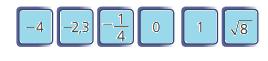
\includegraphics[width=2.79167in,height=0.63542in]{./imgSAEB_8_MAT/media/image1.png}
\end{figure}

Quais deles pertencem ao conjunto:


\begin{escolha}
\item N \rosa{-- $0; 1$}
\item Z \rosa{-- $-4, 0, 1$}
\item Z, mas não pertencem a N? \rosa{$-4$}
\item Q, mas não pertencem a Z? \rosa{$-2,3$ e  $(-\frac{1}{4})$}
\end{escolha}
\num{4} Observe os números abaixo:

$$6; (\sqrt{6}); 6,6; -6$$


Identifique quais deles são:
\begin{escolha}
\item reais e naturais.\rosa{ -- 6}
\item reais e inteiros.\rosa{ -- 6 ; -6}
\item reais e racionais.\rosa{ -- 6; -6; 6,6}
\item reais e irracionais.\rosa{-- $(\sqrt{6})$}
\end{escolha}


\num{5} Complete os espaços abaixo com pertence ou não pertence:


\begin{multicols}{3}
\begin{enumerate}
\def\labelenumi{\alph{enumi}}
\item 100 
\item 100 
\item 100 
\item $(\sqrt{9}) 
$\item $(-\sqrt{9})$ 
\item $(\sqrt{- 9})$ 
\item 2,6 
\end{enumerate}


\begin{enumerate}
\item R*
\item R\textsubscript{+}
\item R\textsubscript{-}
\item R
\item R
\item R
\item R\textsubscript{+}
\end{enumerate}

\begin{enumerate}
\item \rosa{-- Pertence}
\item \rosa{-- Pertence}
\item \rosa{-- Não Pertence}
\item \rosa{-- Pertence}
\item \rosa{-- Pertence}
\item \rosa{-- Não Pertence}
\item \rosa{-- Pertence}
\end{enumerate}
\end{multicols}


\num{6} A representação decimal de um número pode ser: finita, infinita e
periódica ou, ainda, infinita e não periódica. Escreva qual é o caso de
cada um dos números a seguir

\begin{escolha}
\item $(\frac{15}{6})$ \rosa{-- Finita}
\item $(\frac{1}{3})$ \rosa{-- Infinita e periódica}
\item $(\sqrt{3})$ \rosa{-- Infinita e não periódica}
\item $(\sqrt{2})$ \rosa{-- Infinita e não periódica}
\end{escolha}


\num{7} O número (\pi) é classificado como:

\reduline{ uma dízima não periódica.\hfill}

\num{8} O números $121$ é considerado um quadrado perfeito? Por quê?

\reduline{Sim, pois $121 = 11 \cdot 11$.\hfill}

\num{9} O produto ou o quociente de dois números irracionais pode ser um
número racional?


\reduline{ Sim, como exemplos podem ser citados\hfill}

\reduline{ $(\sqrt{2} \cdot \sqrt{2} = \sqrt{2}^2 = 2)$ e também $(\frac{\sqrt{2}}{\sqrt{2}} = 1)$\hfill}


\num{10} Qual é o menor número natural que devemos multiplicar pelo número
125 para que o produto seja um número quadrado perfeito?

\reduline{ $5$, pois $5\cdot 125 = 625$ e $(\sqrt{625}) = 25$.\hfill}

\section{Treino}

\num{1} Qual é a decomposição do número 1 000 em fatores primos?

\begin{escolha}
\item $(2^2\cdot 5^2)$
\item $(2^3 \cdot 5^2 \cdot 2)$
\item $(2^3 \cdot 5^3)$
\item $(2^3 \cdot 5^2)$
\end{escolha}



% SAEB: Compor ou decompor números racionais positivos (representação
% decimal finita) na forma aditiva, ou em suas ordens, ou em adições e
% multiplicações.

% A: Incorreta, pois, o aluno não computou um elemento $2$ e um elemento $5$
% na fatoração..

% B: Incorreta, pois o aluno computou um elemento a mais e um elemento $5$ a
% menos na fatoração.

% C: Correta, pois, ao decompor o número 1.000 em fatores primos, obtemos
% $2^3$ \cdot $5^3$.

% D: Incorreta, pois o aluno não computou um elemento 5 na fatoração.
% -----


\num{2} Sobre o número $123.456.789$, podemos afirmar que:

\begin{escolha}
\item é múltiplo de $5$
\item é múltiplo de $2$
\item é múltiplo de $3$
\item é múltiplo de $10$
\end{escolha}


% 2
% SAEB: Identificar um número natural como primo, composto,
% ``múltiplo/fator de'' ou ``divisor de'' ou identificar a decomposição de
% um número natural em fatores primos ou relacionar as propriedades
% aritméticas (primo, composto, ``múltiplo/fator de'' ou ``divisor de'')
% de um número natural à sua decomposição em fatores primos.

% A: Incorreta, pois o aluno pode realizar a divisão incorretamente do
% valor 123.456.789 e chegar a essa conclusão.

% B: Incorreta, pois o aluno pode realizar a divisão incorretamente do
% valor 123.456.789 e chegar a essa conclusão.

% C: Correta, pois (1 + 2 + 3 + 4 + 5 + 6 + 7 + 8 + 9 = 45). Logo, 45 é
% múltiplo de 3, então

% 123.456.789 também será.

% D: Incorreta, pois o aluno pode realizar a divisão incorretamente do
% valor $123.456.789$ e chegar a essa conclusão.
% ----

\num{3} Manoel ganhou um prêmio na loteria no valor de R\$\,12.500.345.769,00.
Qual algarismo está situado na casa da centena de milhar?

\begin{escolha}
\item $4$
\item $5$
\item $0$
\item $3$
\end{escolha}



%3
% SAEB: Compor ou decompor números racionais positivos (representação
% decimal finita) na forma aditiva, ou em suas ordens, ou em adições e
% multiplicações.

% A: Incorreta, pois, ao contar as casas erroneamente e considerar o
% número uma casa à direita o aluno pode considerar esse.

% B: Incorreta, pois, ao contar as casas erroneamente e considerar o
% número duas casas à direita, o aluno pode considerar esse resultado.

% C: Incorreta, pois, ao contar as casas erroneamente e considerar o
% número uma casa à esquerda, o aluno pode considerar esse resultado.

% D, Correta, pois o número 3 está situado na casa das centenas de milhar.
% ----

\chapter{Operações
aritméticas}

\section{Habilidades do SAEB}

\begin{itemize}
  \item Calcular o resultado de adições, subtrações,
multiplicações ou divisões envolvendo número reais.
\item
  Calcular o resultado de potenciação ou radiciação envolvendo números
  reais.
\item
  Resolver problemas de adição, subtração, multiplicação, divisão,
  potenciação ou radiciação envolvendo número reais, inclusive notação
  científica
\item
  Resolver problemas de contagem cuja resolução envolva a aplicação do
  princípio multiplicativo.
\item
  Resolver problemas que envolvam as ideias de múltiplo, divisor, máximo
  divisor comum ou mínimo múltiplo comum.
\end{itemize}

\subsection{Habilidades da BNCC}

\begin{itemize}
\item EF08MA01, EF08MA02, EF08MA03.
\end{itemize}

Potência de um número racional

Dado um número racional a e um número natural n, a expressão ($a^n$)
chama-se potência e representa uma multiplicação de n fatores iguais ao
número a.

$$(a^n = \frac{a \cdot a \cdot a \cdot a \cdot a \cdot \ldots \cdot a}{n})$$
Essa operação é chamada potenciação.

Assim, pela definição, temos:

$$(10^3 = 10 \cdot 10 \cdot 10 = 1.000)$$

Propriedades da Potenciação:

1ª. propriedade: Produto de potências de mesma base.

Um produto de potências de mesma base pode ser escrito na forma de uma
única potência: conservamos a base e adicionamos os expoentes.

$$(a^m) \cdot (a^n) = (a^{m+n})$$

2ª. Propriedade: Quociente de potências de mesma base

Um quociente de potências de mesma base, em que o expoente do dividendo
é maior ou igual ao expoente do divisor, pode ser escrito na forma de
uma única potência: conservamos a base e subtraímos os expoentes

$$(a^m) \div (a^n) = (a^{m-n})$$ 

com a diferente de zero e m maior ou
igual a n

3ª propriedade: Potência de uma potência.

Um produto de potências de mesma base pode ser escrito na forma de uma
única potência: conservamos a base e multiplicamos os expoentes.

$$(a^m)^n) = (a^{m \cdot n})$$

4ª. propriedade potência de um produto

Para elevar um produto de dois ou mais números racionais a um expoente,
elevamos cada fator a esse expoente.

$$((a \cdot b)^n)= (a^n x b^n)$$

Potências de base dez

A potência de base 10, com expoente natural, é uma maneira de se
escrever o número que, no Sistema de Numeração Decimal, é representado
por 1 seguido de n zeros.

$$(10^5 = 100.000 = 1 + 5...);$$
$$(10^5 = 100.000 = 1 + 5...)$$
$$(10^5 = 100.000 = 1 + 5...)$$

Raiz quadrada exata de um número racional não negativo

Se um número representa um produto de dois fatores iguais não negativos,
então cada fator é a raiz quadrada desse número. Por exemplo:

A raiz quadrada de 25 é 5, pois 

$$(10^5 = 100.000 = 1 + 5...)$$. 

Logo $(10^5 = 100.000 = 1 + 5)$.

A raiz quadrada de 49 é 7, pois:

 $$(10^5 = 100.000 = 1 + 5...)$$. 

 Logo $(\sqrt{49} = 7)$.



\section{Atividades}

\num{1} Calcule o valor das potências abaixo.

\begin{escolha}
\item $\left( - \frac{3}{5}\right )^2$  \rosa{$(\frac{9}{25})$}
\item $( + \frac{1}{2}^5)$  \rosa{$(\frac{1}{32})$}
\item $( - 1\frac{1}{2}^3)$  \rosa{$\left(- \frac{3}{8}\right )$}
\item $( -3,5^2)$  \rosa{$+12,25$}
\item $( + \frac{1}{3}^0)$  \rosa{$1$}
\item $(-1,5^1)$  \rosa{$-1,5$}
\end{escolha}


\num{2} Calcule as operações abaixo.

\begin{escolha}
\item $(( - \frac{1}{2}^2 \; + \; -1^4)$ \rosa{ $(+ 1\frac{1}{4})$}
\item $ - (2^3 . -2^3)$ \rosa{ $(+64)$}
\item $(( - 1\frac{1}{2} . -1^5)$ \rosa{$(+ 1\frac{1}{2})$}
\item $\left ( - \frac{1}{2} \right) \cdot \left( + \frac{3}{2} \right) - \left ( \frac{2}{3} \right)^{3} / \left ( - \frac{1}{27}) \right)$  
    \rosa{$(8 \cdot \frac{3}{8})$}
\item $(0,1) ^2 / (-2) + (1,5) \cdot (-0,1)^2$ \rosa{$0,01$}
\end{escolha}







\num{3} Use a propriedade e, no caderno, escreva cada quociente como uma
única potência e calcule seu valor.


\begin{escolha}
\item $(3^7:3^5)$ 
    \rosa{$(3^{7 - 5} = 3^2 = 3.3 = 9)$     }
\item $(-1^8:-1^6)$ 
    \rosa{$((-1^{8 - 6} = -1^2= -1\cdot-1= +1)$     }
\item $(\left( \frac{2}{3} \right) / \left ( \frac{2}{3} \right)$ 
    \rosa{$((\frac{2}{3})^{4-1}) = ((\frac{2}{3}))^3=(\ (\frac{2}{3}))\cdot(\ (\frac{2}{3}))\cdot(\ (\frac{2}{3})) = (\frac{8}{27})$      }
\item Metade de $(2^10)$ 
    \rosa{$(2^{10} / 2^1 = 2^9 = 2.2.2.2.2.2.2.2.2 = 572)$      }
\item $((-2,5)^5) \div (-2,5)^2$ 
    \rosa{$((-2,5)^{5-2} = (-2,5)^3= (-2,5). (-2,5). (-2,5) = -15,625)$     }
\item $(a^9 \div a^8)$, com a racional não nulo 
    \rosa{$(a^{9-8} = a^1 = a)    $  }
\item $(1^8 \div 1^2)$ 
    \rosa{$(1^{8-2} = 1^6= 1.1.1.1.1.1 = 1)$      }
\item terça parte de $(3^8)$ 
    \rosa{$(3^8-1)= (3^7) = 3.3.3.3.3.3.3 = 2187$     }
\end{escolha}



\num{4} Jamile fez uma viagem turística ao topo de uma montanha. Ao chegar em
certo local, observou uma pedra antiga com o seguinte enunciado: esta
pedra tem o peso de $[(-5)^3]^2\,kg$. Quanto pesa a pedra que Jandira
observou?

\reduline{ Utilizando a propriedade de multiplicação de expoentes temos que:\hfill}
\reduline{ $((-5)^{3.2}= (-5)^6= (-5) . (-5) . (-5) . (-5) . (-5) . (-5)= 15.625 kg)$\hfill}


% -----------------

\num{5} Uma sala de jantar quadrada terá o piso coberto com ladrilhos com
medida de comprimento dos lados de 60 cm.


\begin{escolha}
\item Qual é a medida de comprimento dos lados da sala sabendo que a medida
de área dela é de $81 m^2$?
\item Quantos ladrilhos serão necessários para cobrir o piso?
\end{escolha}

\reduline{ (a) Considerando que a sala é quadrada e que a fórmula da área de um\hfill}
\reduline{ quadrado é $l^2$, para descobrirmos o real valor de cada lado, basta\hfill}
\reduline{ fazermos a operação inversa: $l^2 = 81; l= (\sqrt{81}); l= 9$\hfill}
\reduline{ (b) Se cada lado da sala possui 9 metros e cada lado do ladrilho possui 0,60 cm temos que:\hfill}
\reduline{ $9:0,6 = 15;$ $(15 \cdot 15 = 225$ ladrilhos)\hfill}

\num{6} Utilizando os conhecimentos de redução de potências, reduza as
potencias abaixo.

\begin{escolha}
\item $10^2 \cdot 2^2$  
        \rosa{ $(10 \cdot 2)^2 = 20^2$ }
\item $11^2 \cdot 3^2$  
        \rosa{ $(11 \cdot 3)^2 = 33^2$ }
\item $(-6)^3 . (-8)^3$  
        \rosa{ $((-6) . (-8)) ^3 = 48^3$ }
\item $((3,1)^5 . (0,7)^5 \cdot 2^5)$  
        \rosa{ $((3,1 \cdot 0,7 \cdot 2)^5= 4,34^5)$ }
\end{escolha}





\num{7} Calcule o valor de cada potência com exponente negativo

\begin{escolha}
\item $(8^{-2}$) 
              \rosa{$ (8^{-2} = \frac{1}{8^2}) = (\frac{1}{64})$}
\item $(5^{-1})$ 
              \rosa{$ 5\textsuperscript{-1}= (\frac{1}{5^1}) = (\frac{1}{5})$}
\item $((-2)^{-4}) $
              \rosa{$ ((-2)^{-4} = \frac{1}{2.4} = \frac{1}{16})$}
\item $((\frac{1}{2})^{-3}) $
              \rosa{$ ((\frac{1}{2})^{-3}) = (\frac{2}{1^3}) = (\frac{2}{1}) = 2$}
\item $((-3)^{-3}) $
              \rosa{$ ((-3)^{-3})= (\frac{1}{3^3}) = (\frac{1}{27})$}
\item $(\frac{1}{2}^{-5}) $
              \rosa{$ (\ \frac{1}{2}^{-5}) = (\frac{2}{1}^5) = 32$}
\end{escolha}


\num{8} Calcule as seguintes potências de base 10 e coloque-as em forma
decimal.

\begin{escolha}
\item $(10^6)$
    \rosa{$1 000 000$}
\item $(10^-6)$
    \rosa{$0, 000 001$}
\item $(10^-4)$
    \rosa{$0, 0001$}
\item $(10^4)$
    \rosa{$10 000$}
\item $(10^-2)$
    \rosa{$0,01$}
\item $(10 ^-5)$
    \rosa{$0,00001$}
\item $(10^10)$
    \rosa{$10 000 000 000$}
\item $(10^-8)$
    \rosa{$0,00000001$}
\end{escolha}

\num{9} Reinaldo é professor e, durante uma de suas aulas de estatística,
resolveu demonstrar a população da Terra em formato decimal. Porém, ao
tentar fazer a demonstração, o espaço de sua lousa não foi suficiente.
Sabendo que a população da Terra em 2022 chegou a 8 bilhões, como
poderíamos representar este número para que caiba na lousa?

\reduline{ Reinaldo poderia representar por meio de Notação científica (potência de base 10).\hfill}
\reduline{ Considerando a população da terra como 8.000.000.000, outra forma \hfill}
\reduline{ de reescrever seria $(8 \cdot 10^9)$.\hfill}

\num{10} Felipe é artista e uma de suas obras é conhecida como quadrado
infinito. Ao observar o quadro, um matemático fez as seguintes
descobertas:

\begin{figure}[H]
\centering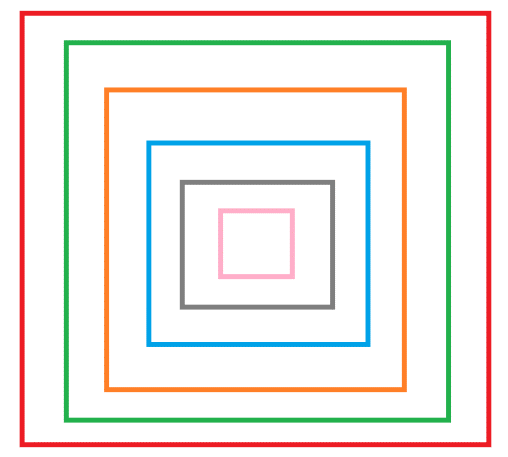
\includegraphics[width=2.3125in,height=2.07917in]{./imgSAEB_8_MAT/media/image2.png}
\end{figure}

O quadrado Vermelho possui uma área de $25\,cm^2$.

O quadrado Verde possui uma área de $22\,cm^2$.

O quadrado Laranja possui uma área de $14\,cm^2$.

O quadrado Azul possui uma área de $64\,cm^2$.

O quadrado Cinza possui uma área de $36\,cm^2$.

O quadrado Rosa possui uma área de $16\,cm^2$.

Com as informações obtidas pelo matemático, responda às perguntas:

\begin{escolha}
\item Perímetro do quadrado vermelho.
        \rosa{  $(\sqrt{256} = 16, 16 \cdot 4 = perímetro = 64)$}
\item Perímetro do quadrado verde.
        \rosa{  $(\sqrt{225}) = 15, 15 \cdot 4 = perímetro = 60$}
\item Perímetro do quadrado laranja.
        \rosa{  $(\sqrt{144}) = 12, 12 \cdot 4 = perímetro= 48$}
\item Perímetro do quadrado azul.
        \rosa{  $(\sqrt{64}) = 8, 8 \cdot 4 = perímetro = 32$}
\item Perímetro do quadrado cinza.
        \rosa{  $(\sqrt{36}) = 6, 6 \cdot 4 = perímetro = 24$}
\item Perímetro do quadrado rosa.
        \rosa{  $(\sqrt{16}) = 4, 4 \cdot 4 = perímetro = 16$}
\end{escolha}

% \reduline{ Para descobrir o perímetro de cada quadrado a solução se mostra a mesma\hfill}
% \reduline{ se temos que a formula da área de um quadrado é l ^2 para descobrirmos o\hfill}
% \reduline{ real valor de cada lado, basta fazermos a operação inversa, no caso a radiciação.\hfill}

\section{Treino}

\num{1} Raul estava passeando pela rua e, ao passar por uma loja de discos
antigos, viu um álbum com o seguinte título: ``Eu Nasci Há Dez Mil Anos
Atrás''. Se a capa desse álbum fosse representada em forma de potência
de base 10, qual o novo nome do álbum?

\begin{escolha}
\item Eu Nasci Há $10^2$ anos Atrás
\item Eu Nasci Há $10^3$ anos atrás
\item Eu Nasci Há $10^4$ anos atrás
\item Eu Nasci Há $10^5$ Anos Atrás
\end{escolha}


SAEB: Resolver problemas de adição, subtração, multiplicação, divisão,
potenciação ou radiciação envolvendo número reais, inclusive notação
científica

BNCC: EF08MA02 -- Resolver e elaborar problemas usando a relação entre
potenciação e radiciação, para representar uma raiz como potência de
expoente fracionário.

A: Incorreta, pois o número de zeros estava errado.

B: Incorreta, pois o número de zeros estava errado.

C: Correta, pois:

$10000 = 10 \cdot 10 \cdot 10 \cdot 10$ ou seja $(10^4)$

D: Incorreta, pois o número de zeros estava errado.

\num{2} Thiago é um professor de matemática e, ao comemorar seu aniversário
com seus alunos, resolveu lançar um enigma. Sua idade seria o expoente
do resultado da seguinte expressão:

$$(\frac{2^{25} \cdot 2^{35} \cdot 2^{30}} {2^2.2^1})$$

Qual é a Idade de Thiago?

\begin{escolha}
\item 2
\item 93
\item 45
\item 30
\end{escolha}

SAEB: Resolver problemas de adição, subtração, multiplicação, divisão,
potenciação ou radiciação envolvendo número reais, inclusive notação
científica

A: Incorreta, pois, ao confundir expoente com base, o aluno chegaria a
esse resultado.

B: Incorreta, pois o aluno chegaria a esse conclusão se somasse todos os
expoentes incorretamente.

C: Incorreta, pois, ao dividir o expoente do numerador por 2 ao invés de
3, o aluno chegaria a esse resultado.

D: Correta pois, utilizando a propriedade de multiplicação e divisão de
potências de mesma base, temos que

No numerador $(2^{25+35+30}=2^{90})$.

No denominador $(2^{2+1}) = 2^3$.

Realizando a divisão, temos que $(2^{90}:3) = (2^{30})$.

Considerando que a idade de Thiago é apenas o expoente, sabemos que
Thiago tem 30 anos.

\num{3} Um pen drive possui diferentes capacidades de memória, mas a medida
normalmente utilizada é o GB. Sabendo que 1 GB = $(2^{10})$ megabytes,
ao comprar um pen drive de 32 GB, quantos megabytes de armazenamento
estarão disponíveis?

\begin{escolha}
\item 32.768 megabytes
    \rosa{ Correta, pois: $(2^10) = 1024$; $1024 \cdot 32 = 32.768$ megabytes.}
\item 32.000 megabytes
    \rosa{ Incorreta, o aluno chegaria a esse resultado ao considerar que $(2^{10})$ seja 1.000 ao invés de 1.024.}
\item 16.384 megabytes
    \rosa{ Incorreta, pois, ao considerar um 2 a menos na expressão, o aluno chegaria a esse resultado.}
\item 64 megabytes
    \rosa{ Incorreta, pois, ao realizar apenas a multiplicação ao\\ invés de realizar o cálculo da potência, o aluno chegaria a esse resultado.}
\end{escolha}

\begin{comment}

SAEB: Resolver problemas de adição, subtração, multiplicação, divisão,
potenciação ou radiciação envolvendo número reais, inclusive notação
científica.

BNCC: EF08MA01 -- Efetuar cálculos com potências de expoentes inteiros e
aplicar esse conhecimento na representação de números em notação
científica.



\chapter{Frações}

\section{Habilidades do SAEB}

\begin{itemize}
\item
  Identificar frações equivalentes.
\item
  Determinar uma fração geratriz para uma dízima periódica.
  \item Representar frações menores ou maiores que a
unidade por meio de representações pictóricas ou associar frações a
representações pictóricas.
\end{itemize}

\subsection{Habilidade da BNCC}

\begin{itemize}
  \item EF08MA051.
\end{itemize}

Comparação de números racionais

Comparar dois números racionais significa estabelecer se entre eles
existe uma relação de superioridade, inferioridade ou igualdade.

Todo número racional negativo é menor que todo número racional positivo

(\frac{1}{5}) \textless{} (\frac{3}{4})

Todo número racional negativo é menor que zero

-5 \textless{} 0 -12,5 \textless{} 0 -(\frac{3}{2}) \textless{} 0

Operações com números racionais

Adição e subtração

Na forma fracionária, temos que estudar dois casos distintos: o primeiro
deles refere-se às frações com denominadores iguais.

O segundo, às frações com denominadores diferentes.

1º. caso: Frações de mesmo denominador.

Para somarmos (ou subtrairmos) frações de mesmo denominador, mantemos o
denominador e somamos (ou subtraímos) os numeradores. Veja um exemplo:

(\frac{3}{5}) + (\frac{6}{5}) = (\frac{9}{5})

2° caso: Frações com denominadores diferentes.

Para somarmos (ou subtrairmos) frações com denominadores diferentes,
devemos obter frações equivalentes às frações dadas, de mesmo
denominador. Em seguida, mantemos o denominador comum e somamos (ou
subtraímos) os numeradores.

(\frac{2}{4}) + (\frac{3}{7}) = (\frac{14 + 12}{28}) =
(\frac{26}{28})

Multiplicação de números racionais

Para multiplicarmos dois números racionais na forma fracionária,
multiplicamos os numeradores entre si e, em seguida, os denominadores.
Caso seja necessário, simplificamos o resultado até obter a fração
irredutível. Exemplo:

(\frac{3}{4}) \cdot (\frac{2}{5}) = (\frac{6}{20})= (\frac{3}{10})

Divisão de números racionais

Para dividirmos dois números racionais na forma fracionária, mantemos a
primeira fração e multiplicamos pelo inverso da segunda.

(\frac{1}{2}) \div (\frac{3}{5})= (\frac{1}{2}) \cdot (\frac{5}{3}) =
(\frac{5}{6})

Dízimas periódicas

Em Matemática, muitas vezes, é útil representar números racionais,
expressos por meio de frações, na forma decimal. Para isso, basta
dividir o numerador pelo denominador. Em alguns casos, essa
representação decimal é finita. Já em outros casos, ela é infinita.
Exemplo:

(\frac{1}{3}) = 0,3333333......

Fração geratriz de dízimas periódicas simples

Vamos encontrar a fração geratriz da dízima periódica 0,333333 ..., ou
seja, encontrar qual fração, quando transformada em número racional na
forma decimal, gera essa dízima.

Para isso, montamos uma equação:

0,333333333... - x

3,33333333... - 10x

3,3333333333... - 0,333333333... = 3

10x - x = 9x

Logo temos que (\frac{3}{9}) simplificando (\frac{1}{3}) é a nossa
fração geratriz.


\begin{comment}


\section{Atividades}

\num{1} Classifique com V para verdadeiro e F para falso as afirmações a
seguir:

( ) 4,9 = 4,09

( ) -15,3 \textless{} 15,3

( ) (\frac{19}{3}) \textgreater{} (\frac{23}{3})

( ) (-\frac{89}{7}) \textless{} \left(- \frac{63}{4}\right )

( ) \left(- \frac{7}{5}\right ) \textgreater{} -1,4

( ) 23,98 \textgreater{} 23,89

==R:

( F ) 4,9 = 4,09

( V ) -15,3 \textless{} 15,3

( F ) (\frac{19}{3}) \textgreater{} (\frac{23}{3})

( V ) (-\frac{89}{7}) \textless{} \left(- \frac{63}{4}\right )

( F ) \left(- \frac{7}{5}\right ) \textgreater{} -1,4

( V) 23,98 \textgreater{} 23,89

\num{2} Efetue as operações a seguir:

\item \left(- \frac{8}{5}\right ) + 2,5 =
\item (\frac{14}{3}) + (\frac{19}{5})
\item -(\frac{8}{13}) - (\frac{3}{5})
\item 79,02 - (\frac{12}{5})
\item 125 - (\frac{35}{4})
\item (\frac{49}{7}) + (\frac{2}{3})
\item 50 - (\frac{1}{2})
\item 100 - (\frac{1}{3})

++R: tiny
\item \left(- \frac{8}{5}\right ) + 2,5 = -(\ \frac{8}{5}) + (\frac{25}{10}) = (\frac{- 16}{10})+(\frac{25}{10}) = (\frac{9}{10})
\item (\frac{14}{3}) + (\frac{19}{5})= (\frac{70}{15}) + (\frac{57}{15}) = (\frac{127}{15})
\item (-\frac{8}{13}) - (\frac{3}{5}) = ( -\frac{40}{65}) - (\frac{39}{65}) = (-\frac{79}{65})
\item 79,02 - (\frac{12}{5}) = (\frac{7.902}{100}) - (\frac{12}{5}) = (\frac{7.902}{100}) - (\frac{240}{100}) = (\frac{7.662}{100})
\item 125 - (\frac{35}{4}) = (\frac{125}{1}) - (\frac{35}{4}) = (\frac{500}{4}) - (\frac{35}{4}) = (\frac{465}{4})
\item (\frac{49}{7}) + (\frac{2}{3}) = (\frac{147}{21}) + (\frac{14}{21}) = (\frac{161}{21})
\item 50 - (\frac{1}{2}) = (\frac{50}{1}) - (\frac{1}{2}) = (\frac{100}{2}) - (\frac{1}{2}) = (\frac{99}{2})
\item 100 - (\frac{1}{3}) = (\frac{100}{1}) - (\frac{1}{3}) = (\frac{300}{3}) - (\frac{1}{3}) = (\frac{299}{3})

\num{3} Resolva as multiplicações abaixo, mas antes de calculá-las,
transforme os decimais em números fracionários.
\item 0,5 \cdot 12,7
\item 3,6 \cdot 6,7
\item 9,3 \cdot 13,25
\item 2,9 \cdot 3,8
\item 11,2 \cdot 4,2
\item 7,5 \cdot 6,6
\item 0,456 \cdot 0,345
\item 0,01 \cdot 0,001

++R:
\item 0,5 \cdot 12,7 = (\frac{5}{10}) . (\frac{127}{10}) = (\frac{635}{100})
\item 3,6 \cdot 6,7 = (\frac{35}{10}) . (\frac{67}{10})
\item 9,3 \cdot 13,25 = (\frac{93}{10}) . (\frac{1325}{100}) = (\frac{123\ 225}{1\ 000})
\item 2,9 \cdot 3,8 = (\frac{29}{10}) . (\frac{38}{10}) = (\frac{1102}{100})
\item 11,2 \cdot 4,2= (\frac{112}{10}) . (\frac{42}{10}) = (\frac{4\ 704}{100})
\item 7,5 \cdot 6,6 = (\frac{75}{10}) . (\frac{66}{10}) = (\frac{4950}{100})
\item 0,456 \cdot 0,345 = (\frac{456}{1\ 000}) . (\frac{345}{1\ 000}) = (\frac{157\ 320}{1\ 000\ 000})
\item 0,01 \cdot 0,001= (\frac{1}{100}) . (\frac{1}{1\ 000}) = (\frac{1}{100\ 000})

\num{4} Resolva as ivisões abaixo, mas antes transforme os decimais em
números fracionários.
\item 0,5 \div 3,4
\item 9,4 \div 3,1
\item 5,1 \div 0,2
\item 0,2 \div 0,1
\item 0,01 \div 0,001
\item 2,1 \div 0,5
\item 4,2 \div 0,1
\item 3,1: 1,5

++R:
\item 0,5 \div 3,4 = (\frac{5}{10}) \div (\frac{34}{10}) = (\frac{5}{10}) . (\frac{10}{34}) = (\frac{50}{340})
\item 9,4 \div 3,1 = (\frac{94}{10}) \div (\frac{31}{10}) = (\frac{94}{10}) . (\frac{10}{31}) = (\frac{940}{310})
\item 5,1 \div 0,2 = (\frac{51}{10}) \div (\frac{2}{10}) = (\frac{51}{10}) . (\frac{10}{2}) = (\frac{510}{20})
\item 0,2 \div 0,1 = (\frac{2}{10}) \div (\frac{1}{10}) = (\frac{2}{10}) . (\frac{10}{1}) = (\frac{20}{10}) = 2
\item 0,01 \div 0,001= (\frac{1}{100}) \div (\frac{1}{1\ 000}) = (\frac{1}{100}) . (\frac{1\ 000}{1}) = (\frac{1\ 000}{100}) = 10
\item 2,1 \div 0,5 = (\frac{21}{10}) \div (\frac{5}{10}) = (\frac{21}{10}) . (\frac{10}{5}) = (\frac{210}{50})
\item 4,2 \div 0,1 = (\frac{42}{10}) \div (\frac{1}{10}) = (\frac{42}{10}) . (\frac{10}{1}) = (\frac{420}{10}) = 42
\item 3,1: 1,5 = (\frac{31}{10}) \div (\frac{15}{10}) = (\frac{31}{10}) . (\frac{10}{15}) = (\frac{310}{150})

\num{5} Transforme as dízimas periódicas abaixo em frações geratrizes:
\item 2,333333...
\item 3,181818...
\item 0,144444...
\item 4,166666...
\item 1,2222...

++R:
\item (\frac{21}{9}) = (\frac{7}{3})
\item (\frac{315}{99})\$
\item (\frac{13}{90})
\item (\frac{375}{90}) = (\frac{25}{6})
\item (\frac{11}{9})

\num{6} Prove que 0,99999999999999 = 1

\reduline{ (\frac{0,99999999}{9,99999999} = \frac{x}{10x})\hfill}
\reduline{ 9,999999999 -- 0,999999999 = 9;  10 x - x = 9 \hfill}
\reduline{ Logo (\frac{9}{9}) = 1\hfill}

% \num{7} Complete com X as lacunas corresponde aos valores corretos

% %Paulo: criar uma tabela com os valores abaixo:
\begin{figure}[H]% 
\centering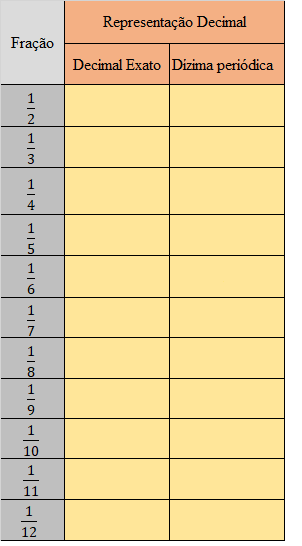
\includegraphics[width=2.37378in,height=4.29167in]{./imgSAEB_8_MAT/media/image3.png}
\end{figure}

% R: 

% %Paulo: criar uma tabela com os valores abaixo:
\begin{figure}[H]% 
\centering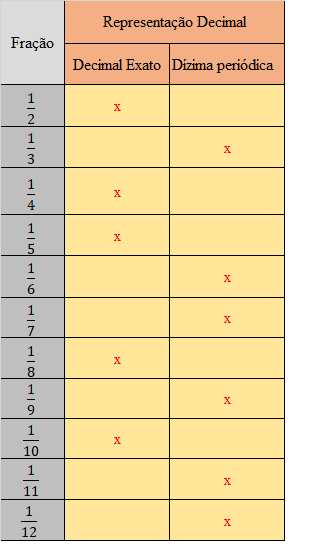
\includegraphics[width=2.14722in,height=3.775in]{./imgSAEB_8_MAT/media/image4.png}
\end{figure}

\num{7} Ao realizar duas operações na calculadora, Juliana obteve os
seguintes resultados: 3,33333333... e 0,8888888...

Quais operações Juliana pode ter realizado?

\reduline{ (\frac{3,333333333}{33,33333333} = \frac{x}{10x})}
\reduline{ 33,33333333... - 3,33333333... = 30}
\reduline{ 10 x - x = 9; Logo, temos que Juliana chegou à fração (\frac{30}{9}),} 
\reduline{ ou equivalentes. Analogamente, temos que }
\reduline{ (\frac{0,888888888}{8,888888888} = \frac{x}{10x}) 8,8888888... -- 0,88888888 = 8; 10x - x = 9}
\reduline{ Logo, temos que Juliana chegou à fração (\frac{8}{9}), ou equivalentes.}

\num{8} Um professor de matemática aposentado resolveu inovar em sua festa de
aniversário. Na parede do salão de festas, colocou um cartaz com os
seguintes dizeres ``ao descobrirem a fração geratriz do número
5,454545..., saberão que o numerador desta fração é a idade que estou
completando hoje''. Quantos anos o professor está completando?


\reduline{5,45454545... \longrightarrow x}
\reduline{545,454545... \longrightarrow 100x}
\reduline{(\frac{5,45454545}{545,454545} = \frac{x}{100x})}
\reduline{5,45454545... - 545,454545 = 540; 100 - x = 99}
\reduline{Logo temos que (\frac{540}{99}) = (\frac{60}{11}), logo, 60 anos.}


\num{9} Marly e João são irmãos gêmeos. Ao divirem tarefas domésticas,
decidiram que cada um ia limpar uma parte da casa, desde que ambos
limpassem ao final a mesma fração que o outro. Sabendo que Marly limpou
(\frac{3}{9}) da casa, qual fração João deverá limpar?

\reduline{ O aluno pode responder qualquer fração equivalente, tal como (\frac{6}{18}).}

\section{Treino}

\num{1} Assinale a alternativa correta:
\item O valor do número (\pi) é aproximadamente
3,14159265358979323846\ldots, e ele é considerado uma dízima periódica
simples, pois seus 3 últimos números são pares.
\item O número de ouro representado pelo número 1.61803399... é considerado
uma dízima periódica simples.
\item Ao calcularmos uma dízima periódica simples, sempre encontramos uma
fração geratriz.
\item O conjunto dos números irracionais é composto por dízimas periódicas
simples.

SAEB: Determinar uma fração geratriz para uma dízima periódica.

BNCC: EF08MA05 -- Reconhecer e utilizar procedimentos para a obtenção de
uma fração geratriz para uma dízima periódica.

A: Incorreta, pois o aluno pode considerar que o número (\pi) seja de
fato uma dízima periódica simples pelo fato de ter números pares na sua
composição.

B: Incorreta, pois o aluno pode não conhecer a diferença entre uma
dízima periódica simples e uma irracional.

C: Correta, pois o conceito foi descrito corretamente.

D: Incorreta, pois o aluno pode não ser capaz de identificar a diferença
entre uma dizima periódica simples e uma irracional.

\num{2} Ao realizar uma palestra, um renomado médico descobriu que apenas
(\frac{2}{3}) dos convidados se consultava regularmente. Tendo em
vista que compareceram 300 pessoas ao evento, quantos participantes não
costumam se consultar?
\item 200
\item 150
\item 600
\item 100

SAEB: Representar frações menores ou maiores que a unidade por meio de
representações pictóricas ou associar frações a representações
pictóricas.

BNCC: EF08MA05 -- Reconhecer e utilizar procedimentos para a obtenção de
uma fração geratriz para uma dízima periódica.

A: Incorreta, pois esse valor corresponde a (\frac{2}{3}) dos
participantes.

B: Incorreta, pois esse valor corresponde à metade dos participantes.

C: Incorreta, pois esse valor corresponde ao dobro dos partcipantes.

D: Correta, pois (\frac{1}{3}) de 300 é igual a 100.

\num{3} Ao fazer um bolo de aniversário, Cecilia utiliza 400 g de farinha de
trigo. Ao dividir este bolo em 22 pedaços, qual fração geratriz
representara a quantidade de farinha em cada pedaço de bolo?

\begin{enumerate}
\def\labelenumi{\alph{enumi})}
\tightlist
\item
  (\ \frac{200}{1})
\end{enumerate}
\item (\frac{1\ 000}{99})

\begin{enumerate}
\def\labelenumi{\alph{enumi})}
\setcounter{enumi}{2}
\tightlist
\item
  (\ \frac{200}{9})
\end{enumerate}
\item (\frac{1\ 800}{101})

SAEB: Determinar uma fração geratriz para uma dízima periódica.

BNCC: EF08MA05 -- Reconhecer e utilizar procedimentos para a obtenção de
uma fração geratriz para uma dízima periódica.

A: Incorreta, pois o aluno pode chegar a esse valor ao calcular
erroneamente a expressão.

B: Incorreta, pois o aluno pode chegar a esse valor ao calcular
erroneamente a expressão.

C: Correta, pois: 400 g \div 22 pedaços = 18,1818181818.\ldots{}

18,181818181818...
-\/-\/-\/-\/-\/-\/-\/-\/-\/-\/-\/-\/-\/-\/-\/-\/-\/-\/-\/- x

1818,18181818...
-\/-\/-\/-\/-\/-\/-\/-\/-\/-\/-\/-\/-\/-\/-\/-\/-\/-\/-\/-\/-\/-\/-100x

(\frac{18,181818181818}{1818,18181818} = \frac{x}{100x})

1818,181818.\ldots{} - 18,18181818... = 1800

100x - x = 99x

Logo, temos (\frac{1\ 800}{99}). Dividindo ambos por 9, temos que
(\frac{200}{9}).

D \div Incorreta, pois o aluno pode chegar a esse valor ao calcular
erroneamente a expressão.


\chapter{Porcentagens}

\section{Habilidade do SAEB} * Resolver problemas que envolvam porcentagens,
incluindo os que lidam com acréscimos e decréscimos simples, aplicação
de percentuais sucessivos e determinação de taxas percentuais.

\subsection{Habilidade da BNCC}

\begin{itemize}
\item EF08MA04.
\end{itemize}

Porcentagem

Porcentagem é a divisão por cem de algo a ser calculado.

Exemplo:

30 \% de uma jarra de suco

40\% de uma barra de chocolate

25 \% de água de um balde

Existem duas formas para realizarmos esse cálculo: pelo método da regra
de 3 simples, ou pelo método multiplicativo de seu corresponde decimal.

Exemplo:

25\% de 300

Pelo método da regra de três simples temos:

(\frac{100%}{25%} \cdot \frac{300}{x}
)

100 x = 25 \cdot 300

100x = 7500

x = 75

Pelo método multiplicativo de seu correspondente decimal temos:

300 . (\frac{25}{100}) = 75

\section{Atividades}

\num{1} Em uma gincana realizada por uma escola, haverá várias modalidades
para os alunos. Ao final das inscrições, 30 alunos escolheram jogar
futsal, 18 alunos escolheram jogar Vôlei, 45 alunos escolheram jogar
basquete e 32 alunos escolheram não participar de nenhuma modalidade.

Calcule então:
\item \% dos alunos que escolheram jogar futsal.
\item \% dos alunos que escolheram jogar vôlei.
\item \% dos alunos que escolheram jogar basquete.
\item \% dos alunos que escolheram não participar de nenhuma modalidade.

Em cada item acima deixar o espaço de 3 linhas para resposta.

++R:
\item (\frac{125}{30} = \frac{100}{x}); 125 . x = 30 \cdot 100; 125x = 3000; x = 24 \%
\item (\frac{125}{18} = \frac{100}{x}); 125 . x = 100 \cdot 18; 125x = 1800; x = 14,4\%
\item (\frac{125}{45} = \frac{100}{x}); 125 x = 4500; x = 36\%
\item (\frac{125}{32} = \frac{100}{x}); 125 . x = 32 \cdot 100; 125x = 3200; x = 25,6\%

\num{2} Marcos é corretor de imóveis. Em janeiro, após ter um grande sucesso
em suas vendas, ele recebeu um aumento de 10\% no salário, que passou a
ser de R\$\,2.178,00. O valor do salário de Marcos antes do aumento era:
\item R\$\,1.980,00
\item R\$\,1.990,00
\item R\$\,2.000,00
\item R\$\,2.100,00

Deixar o espaço de 3 linhas para resposta.

\reduline{ Utilizando a regra de 3 simples, temos que:\hfill}
--R; (\frac{x}{2178} = \frac{100}{110}); Logo, x . 110 = 2178 \cdot 100; 110x = 217 800; x = 1980

\num{3} Após uma apresentação de teatro, 250 espectadores foram entrevistados
e opinaram sobre o show. Veja o resultado dessa pesquisa:

\begin{itemize}
\item
  Ótimo = 105
\item
  Bom = 100
\item
  Regular = 30
\item
  Ruim = 15
\end{itemize}

Calcule a \% de cada opinião:

\reduline{ Ótimo. (\frac{250}{105} = \frac{100}{x}); 250 . x = 100 \cdot 105; 250x = 10 500; x = 42\% \hfill}
\reduline{ Bom: (\frac{250}{100} = \frac{100}{x})\hfill}
\reduline{ 250 . x = 100 \cdot 100; 250x= 10 000; X= 40 \%\hfill}
\reduline{ Regular: (\frac{250}{30} = \frac{100}{x}); 250.x=100 .30; 250x = 3000; x = 12 \%; \hfill}
\reduline{ (\frac{250}{15} = \frac{100}{x}); 250x = 100 \cdot 15; 250 x = 1500; x = 6 \%\hfill}

\num{4} Valdemar é mecânico e adquiriu um carro quebrado pelo valor de
R\$\,10.000,00. Depois que o consertou, resolveu vendê-lo. Ele anunciou o
carro pelo valor de R\$\,16.000,00. Qual é o fator multiplicativo que ele
utilizou?

\reduline{ Utilizando a regra de 3 simples temos que:\hfill}
\reduline{ (\frac{10.000}{16.000} = \frac{100}{x})\hfill}
\reduline{ Logo 10.000 . x = 16.000 \cdot 1.000\hfill}
\reduline{ 10.000x = 1.600.000; x = 160\hfill}

Logo houve um acréscimo de 60\%, então 60 \div 100 = 0,6.

O fator multiplicativo foi de 0,6.

\num{5} Amanda trabalha em uma loja de calçados. Certo dia, seu gerente
ofereceu uma \% fixa de comissão para cada funcionário.para as vendas de
um tênis de 150 reais Amanda obteve uma comissão de 12 reais. Qual \%
fixa Amanda ganhará sobre cada produto?

\reduline{ R: Utilizando a regra de 3 simples, temos que:\hfill}
\reduline{ (\frac{150}{12} = \frac{100}{x})\hfill}
\reduline{ Logo 150 . x = 12 \cdot 100; 150 x = 1.200; x = 8 \%\hfill}

\num{6} Em um colégio, estudam 3.200 alunos, dos quais 1.440 são meninos. O
número de meninas representa quantos \% do total de alunos que estudam
nesse colégio?

\reduline{ R: Utilizando a regra de 3 simples temos que:\hfill}
\reduline{ (\frac{3.200}{1.440} = \frac{100}{x})\hfill}
\reduline{ Logo, 3.200 . x = 1.440 \cdot 100; 3.200x = 144.000; x = 45\% de meninos. Logo, 55\% são meninas.\hfill}

\num{7} Ao terminar o curso na auto escola, Magda realizou uma prova escrita
contendo leis de trânsito. Ela acertou 38 das 50 questões apresentadas.
Sabendo que, para passar na prova escrita, Magda precisava acertar pelo
menos 80\% da prova, ela foi aprovada ou reprovada?

\reduline{ R: Utilizando a regra de 3 simples, temos que:\hfill}
\reduline{ (\frac{50}{38} = \frac{100}{x}). Logo 50 . x = 38 \cdot 100; 50x = 3.800; x = 76\%, logo, Magda foi reprovada.\hfill}

\num{8} Alfredo é professor de educação física em uma escola. Na última aula,
5 dos 40 alunos de uma classe faltaram. Ao registrar as faltas no diário
de classe, quantos \% de faltas Alfredo reportou naquela aula?

\reduline{ R: Utilizando a regra de 3 simples, temos que:\hfill}
\reduline{ (\frac{40}{5} = \frac{100}{x}). Logo 40 . x = 5 \cdot 100; 40x = 500; x = 12,5\% de faltas.\hfill}

\num{9} A primeira edição da Copa do Mundo de Futebol Masculino foi realizada
em 1930. Desse ano até 2023, já foram realizados 22 torneios, sendo que
o Brasil ganhou 5 deles. O número de conquistas brasileiras representa
quantos \% dos torneios realizados?

\reduline{ R: Utilizando a regra de 3 simples, temos que:\hfill}
\reduline{ (\frac{22}{5} = \frac{100}{x})\hfill}
\reduline{ Logo, 22x = 100 \cdot 5; 22x = 500; x = 22,72 \%\hfill}

\num{10} Quanto cada situação abaixo renderá de juros?

\item A quantia de R\$\,1.800, aplicada durante 5 meses, a uma taxa de 2,3\%
ao mês.

\reduline{ Utilizando juros simples temos que}
\reduline{ J = C × i × t}
\reduline{ J= 1800 \cdot 0,023 \cdot 5}
\reduline{ J= 207}

\item A quantia de R\$\,2.450, aplicada durante 2 meses, a uma taxa de 1,96\% ao mês?

\reduline{ J = C × i × t}
\reduline{ J = 2450 \cdot 0,0196 \cdot 2}
\reduline{ J= 96,04}

\section{Treino}

\num{1} A preparação ideal para um suco é 120 mililitros de água para cada 80
mililitros de suco de fruta concentrado. Qual é a taxa percentual de
água para a preparação do suco?
\item 60\%
\item 6\%
\item 0,6\%
\item 0,06\%

SAEB: Resolver problemas que envolvam porcentagens, incluindo os que
lidam com acréscimos e decréscimos simples, aplicação de percentuais
sucessivos e determinação de taxas percentuais.

BNCC: EF08MA04 -- Resolver e elaborar problemas, envolvendo cálculo de
porcentagens, incluindo o uso de tecnologias digitais.

A: Correta, pois, somando os dois líquidos, temos que 120 + 80 = 200.

Utilizando a regra de 3 simples temos que:

(\frac{200}{120} = \frac{100}{x})

Logo 200 . x = 100 \cdot 120

200 x = 12 000

X= 60\%.

B: Incorreta, pois o aluno chegaria a esse resultado caso inserisse um
zero a menos na expressão.

C: Incorreta, pois o aluno chegaria a esse resultado caso inserisse dois
zeros a menos na expressão.

D: incorreta pois o aluno chegaria a esse resultado caso inserisse três
zeros a menos na expressão.

\num{2} Em uma empresa, foi realizada uma eleição para escolher o seu
representante. O candidato vencedor obteve 22 votos, o equivalente a
55\% do total. Quantas pessoas votaram nessa eleição?
\item 12 pessoas
\item 44 pessoas
\item 22 pessoas
\item 55 pessoas

SAEB: Resolver problemas que envolvam porcentagens, incluindo os que
lidam com acréscimos e decréscimos simples, aplicação de percentuais
sucessivos e determinação de taxas percentuais.

BNCC: EF08MA04 -- Resolver e elaborar problemas, envolvendo cálculo de
porcentagens, incluindo o uso de tecnologias digitais.

A: Incorreta, pois o aluno chegaria a essa conclusão realizando a
multiplicação reta na regra de três ao invés de realizar a multiplicação
cruzada.

B: Correta, pois

(\frac{x}{22} = \frac{100}{55})

55 . x = 22 \cdot 100

55x = 2200

x = 44 pessoas votaram nessa eleição

C: Incorreta, pois o aluno poderia chegar a essa conclusão confundindo o
valor de votos ao total real de pessoas que votaram.

D: Incorreta, pois o aluno poderia chegar a essa conclusão confundindo o
valor da porcentagem com o valor total de pessoas na votação.

\num{3} Marcos fez um empréstimo de R\$\,120.000,00, que deverá ser pago com
juros de 1\% ao mês sobre o valor. Sabendo que pagou R\$\,6.000,00 de
juros, quantos meses ele levou para pagar o empréstimo?
\item 5 meses
\item 20 meses
\item 1 200 meses
\item 6 000 meses

SAEB: Resolver problemas que envolvam porcentagens, incluindo os que
lidam com acréscimos e decréscimos simples, aplicação de percentuais
sucessivos e determinação de taxas percentuais.

BNCC: EF08MA04 -- Resolver e elaborar problemas, envolvendo cálculo de
porcentagens, incluindo o uso de tecnologias digitais.

A: Correta, pois, aplicando juros simples, temos que

J = C × i × t

6 000 = 120 000 \cdot 0,01 . x

6 000 = 1200 x

x = 5 meses

B: Incorreta, pois o aluno chegaria a essa conclusão caso não realizasse
a operação de 1\% \div 100.

C: Incorreta, pois o aluno chegaria a essa conclusão caso multiplicasse
120.000 por 0,01.

D: Incorreta, pois o aluno chegaria a essa conclusão caso considerasse
que o valor dos juros a 1\% ao mês.


\chapter{Equações polinomiais de 1º.
grau}

Habilidades do SAEB * Resolver uma equação polinomial de 1º grau.

\begin{itemize}
\item
  Inferir uma equação, inequação polinomial de 1º grau ou um sistema de
  equações de 1º grau com duas incógnitas que modela um problema.
\item
  Associar uma equação polinomial de 1º grau com duas variáveis a uma
  reta no plano cartesiano.
\item
  Resolver problemas que possam ser representados por sistema de
  equações de 1º grau com duas incógnitas.
\end{itemize}

Habilidades da BNCC EF08MA07, EF08MA08.

Sistemas de equações do 1º. grau com duas incógnitas

Denominamos equação do 1º. grau com duas incógnitas (x e y) aquela que
pode ser reduzida a uma equação do tipo ax + by = c, em que a, b e c são
números reais, chamados coeficientes, com a diferente de 0 e b diferente
de 0.

Exemplo:

Mariana comprou uma caneta e dois lápis por R\$\,10,00.

Indicando por x o preço de uma caneta e por y o preço de um lápis,
podemos escrever:

X + 2y = 10

Temos, então, um exemplo de equação do 1º. grau com duas incógnitas.

Sistema de duas equações do 1º. grau com duas incógnitas

Um sistema geralmente é formado por uma situação-problema que envolve 2
incógnitas. Por exemplo:

Um grupo de amigos foi a uma sorveteria e comprou sorvetes com uma ou
duas bolas ao preço de R\$~3,00 e R\$~5,00, respectivamente. Foram
comprados 12~sorvetes, que custaram ao todo R\$~44,00. Quantos sorvetes
com uma bola foram comprados? E~com duas bolas? Sendo que x = a
quantidade de sorvetes com uma bola e y = a quantidade de sorvetes com
duas bolas.

Assim, podemos representar essa situação em linguagem algébrica da
seguinte forma:

X + y = 12

3x + 5y = 44

Temos, portanto, duas equações do 1º. grau com as mesmas duas
incógnitas, que formam um sistema.

Resolução de Sistemas de equações

Método da substituição

Considere o sistema

x - y = -5

2x + 3y = 10

Enumeramos com I a primeira equação e II a segunda equação.
Primeiramente, isolaremos 1 incógnita da primeira equação. Temos que:

x - y = - 5

x = y - 5

Agora, substituiremos o valor de x na segunda equação:

2x + 3y = 10

2 ( y -- 5) + 3y = 10

2y - 10 + 3y = 10

5y = 20

y = 4

Como sabemos o valor de y, agora basta substituir o valor de y em
qualquer uma das duas equações para obtermos x = -1.

Resolução pelo método da adição

Considere o sistema

X + y = 16

X - y = 2

Realizando a soma das equações membro a membro, obtemos

x + y = 16

x - y = 2

2x + 0y = 18

Temos então que 2x = 18, logo x = 9

Substituindo o valor de x em qualquer uma das equações, obtemos que y =
7.

\section{Atividades}

\num{1} Classifique cada um destes sistemas de equações em determinado,
indeterminado ou impossível, sendo x e y números racionais.
\item x - 2y = 3

3x - 6y = 9
\item 3x - 2y = 1

6x - 4y = 3
\item x - 2y = 3

x + 2y = 7
\item 2x - y = 5

-2x + y = -5

++R:
\item Indeterminado
\item Impossível
\item Determinado: solução \{5,1\}
\item Indeterminado

\num{2} Há 5 anos, Thais tinha a metade da idade que terá daqui a 8 anos.
Qual é a idade de Thais?

\reduline{  extraindo as informações do enunciado, temos que:}
\reduline{ x- 5 = (\frac{x + 8}{2})}
\reduline{ 2( x-5) = x+8}
\reduline{ 2x -10 = x + 8}
\reduline{ 2x -- x= +10 + 8}
\reduline{ x = 18}

\num{3} Um campo de golfe tem medida de perímetro de 300 metros. A medida de
comprimento da largura desse campo é o dobro da medida de comprimento da
profundidade. Quais são as medidas das dimensões desse campo?

\reduline{ Cálculo do perímetro}
\reduline{ 300= 2x + 2x + x + x; 300 = 6x; x = 50}
\reduline{ Logo, as dimensões do campo são 50 m de profundidade e 100 m de largura.}

\num{4} Um tanque de leite tem medida de capacidade de 1.000 litros. Com ele
inicialmente cheio, foram retirados 10 baldes de leite de mesma medida
da capacidade, restando 850 litros no tanque. Qual é a medida de
capacidade de cada balde?

\reduline{ 1000 - 10 x = 850}
\reduline{ -10x = -150}
\reduline{ x = 15}

\num{5} Determine x e y para que cada uma das igualdades seja verdadeira.
\item (x, y ) = ( 8, -3)
\item (7, y + 6) = (x, 9)
\item (x, -2) = (6, y)
\item (x + 1, y + 1) = (6, 4)
\item (x, y + 2) = (5, 4)
\item (4, y + 7) = (x + 1, 6)

Em cada item acima deixar o espaço de 2 linhas para resposta.

Respostas
\item x = 8 e y = - 3
\item x = 7 e y = 3
\item x = 6 e y = -2
\item x = 5 e y = 3
\item x = 5 e y = 2
\item x = 3 e y = -1

\num{6} Hoje, Reinaldo tem o dobro menos quatro anos da idade de Luan. Há dez
anos, a idade de Reinaldo era o triplo da idade de Luan. Quantos anos
eles têm hoje?

\reduline{ Definindo como x a idade de Reinaldo e y a idade de Luan, temos que:}
\reduline{ x = 2y - 4  }
\reduline{ x - 10 = 3(y - 10)}
\reduline{ 2y - 4 - 10 = 3(y - 10) \Rightarrow  2y - 14 = 3y -30 \Rightarrow  -y = -16 \Rightarrow  y = 16}
\reduline{Luan tem 16 anos. Substituindo y por 16, encontramos que}
\reduline{x = 2y - 4  \Rightarrow  x= 2 \cdot 16 - 4  \Rightarrow  x = 28}
\reduline{ Logo, a idade de Reinaldo é 28 anos. }

\num{7} Um estádio de futebol oferece dois valores de ingresso: um para os
torcedores do time mandante e outro para os torcedores da equipe visitante. Um
grupo composto por seis torcedores da equipe mandante e um da torcida
visitante pagou R$\,71,00 pelos ingressos. Outro grupo, de sete torcedores da
equipe mandante e quatro da torcida visitante, pagou R$\,131,00. Qual era o
preço de cada~ingresso?

\reduline{ R: Definindo x para torcida da equipe mandante e y para torcida da equipe\hfill}
\reduline{ visitante, temos que: 6x + y = 71; 7x + 4y = 131\hfill}
\reduline{ Utilizando a equação 1, isolamos o termo y: 6x + y = 71; y = 71 - 6x\hfill}
\reduline{ Utilizando a expressão na equação 2, temos que 7x + 4y = 131; 7x + 4 ( 71 -- 6x) = 131; \hfill}
\reduline{ 7x + 284 - 24x = 131; -17x = - 153; x = 9\hfill}
\reduline{ Logo, o valor do ingresso pago pela torcida da equipe mandante foi de R\$\,9,00.\hfill}
\reduline{ Para encontrarmos o valor do ingresso da torcida visitante:\hfill}
\reduline{ 6x+ y = 71; 6 \cdot 9 + y = 71; 54 + y = 71; y = 17\hfill}
\reduline{ Logo, o valor do ingresso pago pela torcida da equipe visitante foi de R\$\,17,00.\hfill}

\num{8} Resolva os sistemas de equações utilizando o método da substituição.
\item 2x + y = 0

2x - y = 4
\item x - y = 5

x + y = 7
\item x + y = 0

2x + y = 14
\item 4x - y = 6

4y = 8

R:
\item ( 1, -2)
\item (6,1)
\item (14, - 14)
\item ( 2, 2)

\num{9} Em um pátio, há carros e motos, totalizando 32 veículos e 88~pneus.
Determine o número de veículos de cada tipo.

R: Determinando x para motos e y para carros, temos que :
2x + 4y = 88; x + y = 32
Isolando um termo na segunda equação, temos que: x = 32 - y
Inserindo a equação 2 dentro da equação 1, temos:
2(32 - y) + 4y = 88; 64 - 2y + 4y = 88; 2y = 24; y = 12
Portanto, há 12 carros no pátio.
Se o número de veículos no pátio é 32 e já sabemos que há 12 carros,
analogamente, concluímos há 20 motos.

\num{10} Tenho vacas e galinhas, totalizando 35 cabeças e 110 pés. Calcule o
número de~vacas e galinhas.

\reduline{ R: definindo com x = vacas e y = galinhas, temos o seguinte sistema: 4x + 2y = 110; X + y = 35\hfill}
\reduline{ Isolando x na segunda equação: x = 35 - y\hfill}
\reduline{ Substituindo a segunda equação na primeira: 4(35 - y) + 2y = 110; 140 - 4y + 2y = 110; -2y = - 30; y = 15\hfill}
\reduline{ Se o número de galinhas é igual a 15 e temos 35 cabeças, logo, 35 - 15 = 20\hfill}

\section{Treino}

\num{1} Dois tambores contêm juntos 900 litros de petróleo. Se passarmos 100
litros do primeiro tanque para o segundo, este ficará com o dobro do de
litros do primeiro. Quantos litros contém o segundo tanque?
\item 400
\item 500
\item 200
\item 1.000

SAEB: Resolver problemas que possam ser representados por sistema de
equações de 1º grau com duas incógnitas.

BNCC: EF08MA08 -- Resolver e elaborar problemas relacionados ao seu
contexto próximo, que possam ser representados por sistemas de equações
de 1º grau com duas incógnitas e interpretá-los, utilizando, inclusive,
o plano cartesiano como recurso.

A: Incorreta, epis sse seria o resultado em litros do primeiro tanque.

B: Correta, pois, definindo como x e y os tanques, temos que:

x + y = 900 x - 100 = y + 100 y + 100 = 2. (x - 100)

Isolando o termo y temos que: y + 100 = 2x- 200 y = 2x - 200 - 100 = 2x
- 300

Substituindo y na primeira equação x + y = 900 x + 2x - 300 = 900 3x =
900 + 300 = 1.200 x = 1.200 \div 3 x = 400

Analogamente, temos que x + y = 900 400 + y = 900 y = 900 - 400 y = 500
L

C: Incorreta, pois o aluno chegará a essa conclusão ao errar o jogo de
sinal na equação final.

D: Incorreta, pois o aluno chegaria a essa conclusão ao somar os valores
do enunciado sem ao mesmo tentar realizar as operações.

\num{2} Luzia pensou em um número racional. Somou (\frac{1}{3}) a ele e
obteve 11. Em qual número Luzia pensou?
\item (\frac{11}{3})

\begin{enumerate}
\def\labelenumi{\alph{enumi})}
\setcounter{enumi}{1}
\tightlist
\item
  (\frac{3}{11})
\end{enumerate}
\item (\frac{32}{3})

\begin{enumerate}
\def\labelenumi{\alph{enumi})}
\setcounter{enumi}{3}
\tightlist
\item
  (\frac{1}{33})
\end{enumerate}

SAEB: Resolver problemas que possam ser representados por sistema de
equações de 1º grau com duas incógnitas.

BNCC: EF08MA08 -- Resolver e elaborar problemas relacionados ao seu
contexto próximo, que possam ser representados por sistemas de equações
de 1º grau com duas incógnitas e interpretá-los, utilizando, inclusive,
o plano cartesiano como recurso.

A:Incorreta, pois o aluno pode confundir as operações e realizar a
operação de multiplicação .

B: Incorreta, pois o aluno pode esquecer de realizar o m.m.c. e chegar a
essa conclusão.

C: Correta, pois, extraindo as informações do enunciado, temos que:

X + (\frac{1}{3}) = 11

x = 11 - (\frac{1}{3})

x = (\frac{32}{3})

D: Incorreta, pois o aluno pode confundir as operações e realizar a
operação de divisão .

\num{3} Qual é o valor de x que torna verdadeira a igualdade 2x - 7 = -2,5x +
2?
\item x = 18
\item x = 2
\item x = 1,1111111.\ldots.
\item x = 40,5

SAEB: Resolver uma equação polinomial de 1º grau.

BNCC: EF08MA07 -- Associar uma equação linear de 1º grau com duas
incógnitas a uma reta no plano cartesiano.

A: Incorreta, pois, durante a resolução da equação, caso o aluno erre o
sinal de 2,5 e passe o negativo, o valor final será esse.

B: Correta, pois, realizando as operações algébricas, temos que:

2x - 7 = -2,5x + 2

4,5x = 9

x = 2

C: Incorreta, pois, durante a resolução da equação, caso o aluno erre o
sinal de -7 e passe o negativo, o valor final será esse.

D: Incorreta, pois, caso o aluno, no final da expressão, passe o valor
4,5 multiplicando ao invés de dividir, chegará a esse resultado.


\chapter{Representações
algébricas}

Habilidades do SAEB * Identificar uma representação algébrica para o
padrão ou a regularidade de uma sequência de números racionais ou
representar algebricamente o padrão ou a regularidade de uma sequência
de números racionais.

\begin{itemize}
\item
  Identificar representações algébricas equivalentes.
\item
  Resolver problemas que envolvam cálculo do valor numérico de
  expressões algébricas.
\end{itemize}

Habilidades da BNCC EF08MA10, EF08MA11.

Expressões Algébricas

Expressões algébricas são aquelas que indicam operações matemáticas com
números e letras ou somente letras.

É possível usar letras para representar números reais desconhecidos, que
chamamos de incógnitas.

Monômios

Um monômio é uma expressão matemática que consiste em um único termo.
Cada monômio é composto por um coeficiente multiplicado por uma ou mais
variáveis elevadas a expoentes não negativos.

Em um monômio, distinguimos: o coeficiente, que corresponde à parte
numérica (que é um número real); a parte literal, que corresponde a uma
variável ou um produto de variáveis, com expoente natural.

Exemplo:

2x

2 = coeficiente x = parte literal

Adição e subtração de monômios

Uma expressão algébrica em que todos os monômios são semelhantes pode
ser simplificada adicionando ou subtraindo os coeficientes.

Se uma expressão tem monômios semelhantes e monômios não semelhantes,
efetuamos a adição ou a subtração dos semelhantes e conservamos os
demais. Dizemos, então, que foi efetuada uma redução de termos
semelhantes.

Exemplos

2x + 5x = ?

Como são semelhantes, podemos somar os coeficientes e manter a parte
literal, logo temos:

2x + 5x = 7x

Exemplo 2

3x + 5x + 6y = ?

Como nem todos os membros são semelhantes, juntaremos apenas os
semelhantes e conservamos os monômios não semelhantes:

3x + 5x + 6y = 8x + 6y

Polinômios

Expressões algébricas formadas por um monômio ou pela adição e/ou
subtração de monômios são chamadas de polinômios.

Exemplos de polinômios:

4x^2 + 8

X^2 - 8y + 12

A^2 + 5a^2b + 3ab^2 + b^3

\section{Atividades}

\num{1} Dalva tem 44 anos. Escreva uma expressão algébrica que representa a
idade que ela teve há x anos e a idade que ele terá daqui a y anos,
sendo x e y números naturais.

\reduline{ R: Considerando a forma algébrica de solução, temos que:\hfill}
\reduline{ Idade que Dalva já teve: 44 - x\hfill}
\reduline{ Idade que Dalva ainda vai ter: 44 + y\hfill}

\num{2} Celso comprou 1 calça de R\$\,150,00 e 2 camisas.
\item Usando a letra x, escreva uma expressão algébrica que represente o
valor a ser pago nessa situação.
\item O que representa a letra x neste caso?
\item Se o preço de 1 camisa é de R\$\,80,00, quanto ele gastou?

++R: 
\item Utilizando a forma algébrica, temos que150 + 2x.
\item A letra x representa o preço de cada camisa.
\item Se o preço de cada camisa é R\$\,80,00, temos que:

150 + 2 \cdot 80 = 150 + 160 = 310

Celso gastou R\$\,310,00

\num{3} Em um retângulo, o comprimento de um lado mede 4 cm a mais do que o
outro. Representando por x a medida de comprimento, em centímetros, do
menor lado, escreva as expressões algébricas que representam:
\item a medida de comprimento, em centímetros, do maior lado.
\item a medida de perímetro, em centímetros, do retângulo.
\item medida de área, em centímetros quadrados, da região retangular
correspondente.

++R:
\item Utilizando a forma algébrica, temos que:
Como não sabemos as medida de cada lado do retângulo, denominamos seu
lado de x. Como o enunciado nos diz que um dos lados é 4 cm maior que o
outro, temos que o lado maior é
x + 4
\item Considerando os valores do enunciado, temos que
lado maior x + 4
lado menor = x
perímetro= x + 4 + x + 4 + x + x =
Perímetro = 4x + 8
\item considerando que a área do retângulo é l . l, que o lado maior = x +
4 e o lado menor = x:
x + 4 . x =
(x+4) . x
X^2 + 4x

\num{4} Escreva o coeficiente e a parte literal de cada monômio.
\item xy
\item \left(- \frac{2}{3\right }t^2)
\item -c^2 d ^3
\item (\frac{a^2}{5})
\item-10 a\textsuperscript{4}
\item (\frac{2}{3}.{xy})
\item x^3
\item - 20ab
\item 1,5xy^2
\item a^2b^2

R:
\item
Coeficiente: 1
Parte literal: xy
\item Coeficiente: (\frac{- 2}{3})
Parte literal: t^2
\item Coeficiente: -1
Parte literal: c^2d^3
\item Coeficiente: (\frac{1}{5})
Parte literal:a^2
\item Coeficiente: -10
Parte literal:(a^4)
\item Coeficiente: (\frac{2}{3})
Parte literal: xy
\item Coeficiente: 1
Parte literal: x^3
\item Coeficiente:-20
Parte literal: ab
\item Coeficiente: 1,5
Parte literal: xy^2
\item Coeficiente: 1
Parte literal: a^2b^2

\num{5} Escreva o nome de cada polinômio de acordo com o número de termos:
\item 6x^2 - 4x +9
\item 7x^2 + 5 x
\item (4x^4)
\item -3r + (\frac{1}{2})
\item -2abc
\item x^3 + x^2 - x + 1
\item -(\frac{2}{5}) a^2b
\item a + b - 5
\item 3x - y
\item 7x + 8x

++R:
\item trinômio
\item binômio
\item monômio
\item binômio
\item monômio
\item polinômio de 4 termos
\item monômio
\item trinômio
\item binômio
\item monômio

\num{6} Escreva cada polinômio na forma reduzida.
\item 2x^2 - 5x + 3 - 3x^2 - 3 + 7x
\item 3y^3 + 2y^2 + y - 1 - 3y^3 - y^2 - 5y +3
\item - 5xy + 2y^2 + xy - 3y^2 + 2 + 3xy - 1
\item 4x^3 - 5y - 6x^3 + 7y + 3x^3 - 2y
\item 2x^2 - 3x^2 -5x +7x +3 - 3 -x^2 +2x
\item 3x^3 - 3^3 + 2y^2 -y^2 - 5y + y - 1 + 3y^2 - 4y + 2
\item 2y^2 - 3y^2 + xy - 5xy + 3xy - 1 + 2

\begin{itemize}
\tightlist
\item
  y^2 - xy^2 + 1
\end{itemize}
\item 4x^3 - 6x^3 + 3x^3 - 5y + 7y - 2Y

\num{7} Reescreva as expressões abaixo colocando-as em evidência.

\begin{enumerate}
\def\labelenumi{\alph{enumi})}
\tightlist
\item
  ax + ay
\end{enumerate}
\item 16x^2 + 20y^2
\item 5x + 15y - 10z
\item 4x - 16

\begin{enumerate}
\def\labelenumi{\alph{enumi})}
\setcounter{enumi}{4}
\tightlist
\item -5x^3y + 20x^2y^2
\end{enumerate}

++R: Colocando as expressões em evidência, obtemos:
\item a(x+y)
\item 4(4x^2 + 5y^2)
\item 5(x+3y-2z)
\item 4(x-4)
\item 5x^2y(-x+4y)

\num{8} Durante uma aula de matemática, um professor resolveu demonstrar
outra forma de calcular a operação (41 \cdot 39) e escreveu seus cálculos na
lousa assim:

41 \cdot 39 = (40 + 1) (40 - 1) = 40^2 - 1^2 = 1.599

Seguindo a mesma forma exposta pelo professor, calcule os seguintes
produtos:
\item 57 \cdot 63
\item 52. 48
\item 42 \cdot 34

R:
\item 57 \cdot 63 = (60 - 3). (60 + 3) = 60^2 - 3^2 = 3.591
\item 52 \cdot 48 = (50 + 2) . (50 - 2) = 50^2 - 2^2 = 2.496
\item 42 \cdot 34 = (38 + 4) . (38 - 4) = 38^2 - 4^2 = 1.428

\num{9} Uma construtora resolveu comprar dois terrenos de formato retangular
para construir 2 condomínios. Qual é a equação que representa a área
total dos dois terrenos somados?

\begin{figure}[H]
\centering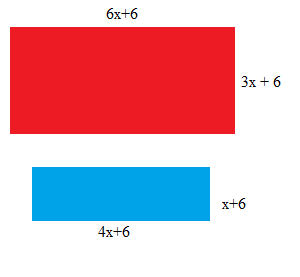
\includegraphics[width=2.04167in,height=1.8873in]{./imgSAEB_8_MAT/media/image5.png}
\end{figure}

\reduline{ R: Considerando que a fórmula da área de um retângulo é l . l, temos que\hfill}
\reduline{ Terreno vermelho: (6x + 6) . (3x + 6)= 18x^2 + 18x + 18x + 36= 18x^2 + 36x + 36\hfill}
\reduline{ Terreno azul: (4x + 6) . (x + 6) = 4x^2 + 24x + 6x + 36 = 4x^2 + 30x + 36 =...\hfill}
\reduline{ Somando os dois terrenos, temos que 18x^2 + 36x + 36 + 4x^2 + 30x + 36 =...\hfill}
\reduline{ Área total dos dois terrenos = 22x^2 + 66x + 72\hfill}

\num{10} Efetue os monômios descritos abaixo:
\item (6x^4+ 12x^6)

\begin{enumerate}
\def\labelenumi{\alph{enumi})}
\setcounter{enumi}{1}
\tightlist
\item
  10xy-xy
\end{enumerate}
\item(6x^3) . (2x^2)
\item ((14x^{10})): (2x^2)
\item (2x^3)^3
\item (-4xy^2) ^3
\item (\frac{30x}{6x}), para x diferente de 0
\item 6x^2 - 8x^2
\item((\frac{4}{5}x)^{-1})

\begin{enumerate}
\def\labelenumi{\alph{enumi})}
\setcounter{enumi}{9}
\tightlist
\item
  9x^2 + 6x^2
\end{enumerate}
\item 7x^2 + 4x
\item (8r) . (6s)

\begin{enumerate}
\def\labelenumi{\alph{enumi})}
\setcounter{enumi}{12}
\tightlist
\item
  (16x^2) :4
\end{enumerate}
\item 8x + 6x + 4x
\item (-4xy^2)^3

++R:
\item (6x^4 + 12x^6 = 18x^{10})
\item 10xy - xy = 9xy

\begin{enumerate}
\def\labelenumi{\alph{enumi})}
\setcounter{enumi}{2}
\tightlist
\item
  (6x^3) . (2x^2) = (12x^5)
\end{enumerate}
\item ((14x^10) \div (2x^2)=7x^8)
\item (2x^3)^3= (2x^9)
\item (-4xy^2)^3= (-4xy^6)
\item (\frac{30x}{6x}), para x diferente de 0 = 5x
\item 6x^2 - 8x^2 = -2x^2
\item((\frac{4}{5}x)^{-1}) = (\frac{5}{4})

\begin{enumerate}
\def\labelenumi{\alph{enumi})}
\setcounter{enumi}{9}
\tightlist
\item
  9x^2 + 6x^2 = 15x^2
\end{enumerate}
\item 7x^2 + 4x^2 = 11x^2
\item (8r) . (6s) = 48rs
\item(16x^2) \div 4 = 4x^2
\item 8x + 6x + 4x = 18x
\item ((-2xy^2)^4)= (16x^4 y^8)

\section{Treino}

\num{1} Elza resolveu comprar uma piscina com as medidas abaixo:

\begin{figure}[H]
\centering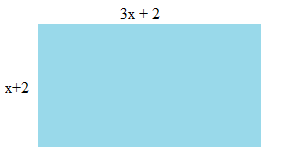
\includegraphics[width=2.9625in,height=1.67014in]{./imgSAEB_8_MAT/media/image6.png}
\end{figure}

Qual é a equação que representa a medida da área em m^2 dessa piscina?
\item 3x^2 + 8x + 4
\item 8x + 8
\item 4x + 4
\item 3x + 1

SAEB: Resolver problemas que envolvam cálculo do valor numérico de
expressões algébricas.

BNCC: EF08MA10 -- Identificar a regularidade de uma sequência numérica
ou figural não recursiva e construir um algoritmo por meio de um
fluxograma que permita indicar os números ou as figuras seguintes.

A: Correta, pois, considerando a medida dos lados, temos que:

3x + 2 . x + 2=

(3x + 2) . (x + 2)=

Utilizando a distributiva:

3x^2 + 6x + 2x + 4

3x^2 + 8x + 4

B: Incorreta, pois o aluno poderia confundir o enunciado e colocar o
resultado do perímetro.

C: Incorreta, pois o aluno poderia realizar uma soma ao invés de uma
multiplicação.

D: Incorreta, pois o aluno poderia chegar a esse valor realizando uma
divisão ao invés de uma multiplicação.

\num{2} Considerando que a^2+ b^2 = 34 e ab= 15, qual é o valor de
(\frac{(a + b)^2}{8}) ?
\item 2,266666666
\item 19
\item 8
\item 9,25

SAEB: Resolver problemas que envolvam cálculo do valor numérico de
expressões algébricas.

BNCC: EF08MA10 -- Identificar a regularidade de uma sequência numérica
ou figural não recursiva e construir um algoritmo por meio de um
fluxograma que permita indicar os números ou as figuras seguintes.

A: Incorreta, pois o aluno chegaria a essa conclusão apenas dividindo um
termo pelo outro.

B: Incorreta, pois o aluno chegaria a essa conclusão realizando apenas a
subtração de um termo pelo outro.

C: Correta, pois

(\frac{(a + b)^2}{8}\ ) = (\frac{a^{2} + 2ab + b^2}{8})

Fazendo a substituição de a^2 + b^2 = 34 e ab = 15, temos que:

(\frac{34 + (2.15)}{8} =) (\frac{34 + 30}{8}) = (\frac{64}{8}) = 8

D: incorreta, pois foi realizada a soma ao invés da multiplicação no
último termo.

\num{3} O diâmetro de um disco de vinil é igual a (x^2 - 3). A partir desse
valor, quanto valem o perímetro e a área do disco?

Considere (\pi) = 3
\item (Área = 3x^4 - 18x^2 - 27 \;Perímetro= 6x^2 - 18)
\item (Área = 3x^4 - 18x^2 + 27 \;Perímetro= 6x^2 + 18)
\item (Área = 3x^4 + 18x^2 + 27 \;Perímetro= 6x^2 - 18)
\item (Área = 3x^4 - 18x^2 + 27 \;Perímetro= 6x^2 - 18)

SAEB: Resolver problemas que envolvam cálculo do valor numérico de
expressões algébricas.

BNCC: EF08MA10 -- Identificar a regularidade de uma sequência numérica
ou figural não recursiva e construir um algoritmo por meio de um
fluxograma que permita indicar os números ou as figuras seguintes.

A: Incorreta, pois o aluno, ao errar o jogo de sinal no cálculo da área,
encontrará esse valor.

B: Incorreta, pois o aluno, ao errar o jogo de sinal no cálculo do
perímetro, encontrará esse valor.

C: Incorreta, pois o aluno, ao errar o jogo de sinal no cálculo da área,
encontrará esse valor.

D: Correta, pois, para o cálculo da área, temos:

(A = \pi r^{2}).

Logo,

A = 3 . (x^2-3) ^2

A = 3 . ((x^4) - 6x^2 + 9)

A = (3x^4) - 18x^2 + 27

Perímetro

P= 2(\text{\ π\ .\ r})

P = 2 \cdot 3. (x^2-3)

P = 2 . (3x^2 - 9)

P = 6x^2 - 18


\chapter{Equações polinomiais de 2º.
grau}

Habilidades do SAEB * Inferir uma equação polinomial de 2º. grau que
modela um problema.

\begin{itemize}
\item
  Resolver uma equação polinomial de 2º. grau.
\item
  Resolver problemas que possam ser representados por equações
  polinomiais de 2º grau.
\end{itemize}

Habilidade da BNCC EF08MA09.

Equação polinomial de 2º. grau

São consideradas equações polinomiais de 2º. grau aquelas encontradas na
forma ax^2 + b = 0

Por exemplo:

Qual é a solução da equação x^2 - 9 = 0, no conjunto R?

Temos que:

X^2 - 9 = 0

X^2 = 9

x = (\sqrt{9})

x = ± 3

O conjunto solução é \{- 3, 3\}

Resolução da equação 16x^2 - 1 = 0

16x^2 = 1

x = (\  \pm \sqrt{\frac{1}{16}})

x = (\  \pm \frac{1}{4})

Logo, o conjunto solução é (+ \frac{1}{4}) e (- \ \frac{1}{4})

\section{Atividades}

\num{1} Determine a solução da equação x^2 + 4 = 0 no conjunto R.

R: x^2 + 4 = 0; X^2 = - 4; X= (\sqrt{- 4})

Como (\sqrt{- 4}) não existe no conjunto R, não temos valores reais
para x. Logo, a equação não tem raízes reais. Assim, S = 0.

\num{2} Resolva, no conjunto R, a equação (2y + 1)^2 = 8 + 2(2y + 1).

\reduline{ R: (2y + 1)(2y + 1) = 8 + 2(2y + 1); 4y^2 + 2y + 2y + 1 = 8 + 4y + 2; 4y^2 + 4y + 1 = 10 + 4y; \hfill}
\reduline{ 4y^2 + 4y - 4y + 1 - 10 = 0; 4y^2 - 9 = 0; Y = ± (\sqrt{\frac{9}{4}}); Y= ± (\frac{3}{2})\hfill}

Logo os números + (\frac{3}{2}) e (\frac{3}{2}) são as raízes da
equação.

\num{3} Determine o conjunto solução de cada uma das seguintes equações do
2°. grau, no conjunto R.
\item x^2 - 1 = 0
\item x^2 - 16 = 0
\item x^2 - 64 = 0
\item 9x^2 = 25

R:
\item \{ -1,1\}
\item \{ -4, 4\}
\item \{-8, 8\}
\item \{\left(- \frac{5}{3}\right ) ,(\frac{5}{3}) \}

\num{4} Identifique a, b e c nas funções quadráticas abaixo:
\item x^2 - 5x + 6 = 0
\item -2x^2 + 8x - 8 = 0
\item x^2 = 4
\item x^2 - x = - (x + 15)

Deixar o espaço de 4 linhas para a resposta.

R:
\item
A = 1
B = -5
C = 6
\item
A = -2
B = 8
C = -8
\item
A = 1
B = 0
C = 4
\item
A = 1
B = 0
C = 15

\num{5} A idade do filho mais novo de Joana é representado pela equação x^2 -
100 = 0. Qual é a idade do filho mais novo de Joana?

\reduline{ R: Realizando a equação temos que:\hfill}
\reduline{ X^2 - 100 = 0; X^2 = 100; x = (\sqrt{100}); x = ±10\hfill}

Como a idade não pode ser representada, com números negativos, temos que
a idade do filho mais novo de Joana é 10 anos.

\num{6} Marcos é dono de uma madeireira que vende blocos de madeira de 2
tamanhos diferentes. Os tamanhos são definidos, em metros, pelas raízes
da equação x^2 - 5x + 4 = 0. Quais são os tamanhos de madeira disponíveis
na madeireira de marcos?

\reduline{ R: Temos que: x^2 - 5x + 4 = 0\hfill}
\reduline{ A = 1; B = - 5; C = 4\hfill}

(\frac{- ( - 5) \pm \sqrt{{- 5}^{2} - 4.\ 1.4}}{2.1})

(\frac{5 \pm \sqrt{25 - 16}}{2})

(\frac{5 \pm \sqrt{9}}{2})

(\frac{5 \pm 3}{2})

(X~1~) = (\frac{5 + 3}{2})= (\frac{8}{2}) = 4

(X~2~) = (\frac{5 - 3}{2})= (\frac{2}{2})=1

Logo, os tamanhos disponíveis de madeira são 1 metro e 4 metros.

\num{7} Evandro é corredor. Certo dia, resolveu participar de uma maratona
com seu amigo José. Como Evandro é mais experiente, largou na frente e
abriu certa vantagem. A distância de Evandro e José em km é definida
pela equação X^2 - 4x + 4 = 0. Sendo assim, quantos km Evandro está na
frente de José?

\reduline{ R: x^2 - 4x + 4 = 0; A = 1; B = -4; C = 4\hfill}
\reduline{ (\frac{- ( - 4) \pm \sqrt{{( - 4)}^{2} - 4\ .\ 1.\ 4}}{2\ .\ 1})\hfill}
\reduline{ (\frac{4 \pm \sqrt{16 - 16}}{2}); (\frac{4}{2}) = 2 km\hfill}

\num{8} Raiane vai para o trabalho todos os dias a pé. A distância de sua
casa para o seu tralho em km é a soma das raízes da equação 2𝑥^2 − 6𝑥 − 8
= 0. Quantos km Raiane anda por dia para ir ao trabalho?

\reduline{ R: 2𝑥^2 − 6𝑥 − 8 = 0; A = 2; B = -6; C = -8\hfill}
\reduline{ (\frac{- ( - 6) \pm \sqrt{{( - 6)}^{2} - 4.2.( - 8)}}{2.2})\hfill}
\reduline{ (\frac{6 \pm \sqrt{36 + 64}}{4}); (\frac{6 \pm \sqrt{100}}{4}); (\frac{6 \pm 10}{4})\hfill}
\reduline{ X1= (\frac{6 + 10}{4}) = (\frac{16}{4}) = 4; X2= (\frac{6 - 10}{4}) = (\frac{- 4}{4}) = -1\hfill}
\reduline{ Somando ambas as raízes, temos que Raiane anda 3km por dia para ir ao trabalho.\hfill}

\num{9} Divina tem 2 filhas com idades diferentes, representadas pelas raízes
da equação x^2 - 20x + 36 = 0. Quais são as idades das filhas de Divina?

\reduline{ R: x^2 - 20x + 36 = 0\hfill}
\reduline{ A= 1; B= -20; C= 36\hfill}
\reduline{ (\frac{- ( - 20) \pm \sqrt{{( - 20)}^{2} - 4.1.36}}{2.1})\hfill}
\reduline{ (\frac{20 \pm \sqrt{400 - 4.1.36}}{2a})\hfill}
\reduline{ (\frac{20 \pm \sqrt{400 - 144}}{2})\hfill}
\reduline{ (\frac{20 \pm \sqrt{256}}{2})\hfill}
\reduline{ (\frac{20 \pm 16}{2}); X1 = (\frac{20 + 16}{2})= (\frac{36}{2} =) 18; X2 = (\frac{20 - 16}{2}) = (\frac{4}{2}) = 2\hfill}
\reduline{ Logo, as filhas de Divina têm 18 anos e 2 anos.\hfill}

\num{10} Mateus pretende pagar uma dívida com o banco. Ele sabe que o valor

B: Correta, pois, utilizando Bhaskhara, temos:
x^2 - 7x = 0

A = 1

B = - 7

C = 0

(\frac{- ( - 7) \pm \sqrt{{( - 7)}^{2} - 4.1.0}}{2.1})

(\frac{7 \pm \sqrt{49}}{2})

(\frac{7 \pm 7}{2})

X1 = (\frac{7 + 7}{2})\$ = (\frac{14}{2}) = 7

X2 = (\frac{7 - 7}{2}) = 0

Logo, realizando a soma de 7 + 0 = 7, obtemos que Clebinho chutou 7
vezes ao gol.

C: Incorreta, pois o aluno pode chegar a essa conclusão considerando que
o enunciado pede apenas o valor antes de extrairmos as raízes da
equação.

D: Incorreta, pois o aluno pode chegar a essa conclusão esquecendo de
dividir o valor de uma das raízes por 2.

\num{2} Daniel é piloto de corridas de alta velocidade. Em uma certa prova,
ele ficou em 2° lugar. A distância em segundos do primeiro colocado para
Daniel é a soma das raízes da equação 4x^2 + 9x = 0. Quanto tempo depois
do primeiro colocado Daniel Chegou?

\begin{enumerate}
\def\labelenumi{\alph{enumi})}
\tightlist
\item
  0
\end{enumerate}
\item 81
\item 9
\item 2,25

SAEB: Resolver problemas que possam ser representados por equações
polinomiais de 2º grau.

BNCC: EF08MA09 -- Resolver e elaborar, com e sem uso de tecnologias,
problemas que possam ser representados por equações polinomiais de 2º
grau do tipo ax2 = b.
que deve é a soma das raízes da equação X^2 + 4x + 3 = 0 multiplicada por
1.000. Sendo assim, quantos reais Mateus deve ao banco?

\reduline{ R: Utilizando Bhaskhara, temos: X^2 + 4x + 3 = 0; A = 1; B = 4; C = 3\hfill}
\reduline{ (\frac{- 4 \pm \sqrt{4^{2} - 4.1.3}}{2.1})\hfill}
\reduline{ (\frac{- 4 \pm \sqrt{16 - 4.1.3}}{2.1}); (\frac{- 4 \pm \sqrt{4}}{2})\hfill}
\reduline{ X1= (\frac{- 4 + 4}{2}) = 0; X2 = (\frac{- 4 - 4}{2}) = -4\hfill}
\reduline{ Multiplicando por 1.000, temos que -4 \cdot 1000 = - 4000. Logo, Mateus deve R\$\,4.000,00 ao banco.\hfill}

\section{Treino}

\num{1} Clebinho é atacante de um famoso time de futebol. Durante uma
partida, o número de suas finalizações ao gol foi a soma das raízes da
equação x^2- 7x = 0. Quantas vezes Clebinho chutou no gol durante a
partida?
\item 0
\item 7
\item 49
\item 14

SAEB: Resolver problemas que possam ser representados por equações
polinomiais de 2º grau.

BNCC: EF08MA09 -- Resolver e elaborar, com e sem uso de tecnologias,
problemas que possam ser representados por equações polinomiais de 2º
grau do tipo ax2 = b.

A: Incorreta, pois o aluno pode chegar a essa conclusão considerando que
o enunciado pede apenas 1 valor das raízes da equação.


A: Incorreta, pois o aluno pode chegar a essa conclusão considerando que


%% Encontro Felipe Jorge

A: Incorreta, pois o aluno pode chegar a essa conclusão considerando que
o enunciado pede apenas 1 valor das raízes da equação.

B: Correta, pois, utilizando Bhaskhara, temos:

x^2 - 7x = 0

A = 1

B = - 7

C = 0

(\frac{- ( - 7) \pm \sqrt{{( - 7)}^{2} - 4.1.0}}{2.1})

(\frac{7 \pm \sqrt{49}}{2})

(\frac{7 \pm 7}{2})

X1 = (\frac{7 + 7}{2})\$ = (\frac{14}{2}) = 7

X2 = (\frac{7 - 7}{2}) = 0

Logo, realizando a soma de 7 + 0 = 7, obtemos que Clebinho chutou 7
vezes ao gol.

C: Incorreta, pois o aluno pode chegar a essa conclusão considerando que
o enunciado pede apenas o valor antes de extrairmos as raízes da
equação.

D: Incorreta, pois o aluno pode chegar a essa conclusão esquecendo de
dividir o valor de uma das raízes por 2.

\num{2} Daniel é piloto de corridas de alta velocidade. Em uma certa prova,
ele ficou em 2° lugar. A distância em segundos do primeiro colocado para
Daniel é a soma das raízes da equação 4x^2 + 9x = 0. Quanto tempo depois
do primeiro colocado Daniel Chegou?

\begin{enumerate}
\def\labelenumi{\alph{enumi})}
\tightlist
\item
  0
\end{enumerate}
\item 81
\item 9
\item 2,25

SAEB: Resolver problemas que possam ser representados por equações
polinomiais de 2º grau.

BNCC: EF08MA09 -- Resolver e elaborar, com e sem uso de tecnologias,
problemas que possam ser representados por equações polinomiais de 2º
grau do tipo ax2 = b.

A: Incorreta, pois o aluno pode chegar a essa conclusão considerando que
o enunciado pede apenas 1 valor das raízes da equação descrita.

B: Incorreta, pois o aluno pode chegar a essa conclusão considerando que
o enunciado pede apenas o valor antes de extrairmos as raízes da equação
descrita.

C: Incorreta, pois o aluno pode chegar a essa conclusão esquecendo de
dividir o valor de uma das raízes por 4.

D: Correta, pois, utilizando Bhaskhara, temos:

4x^2 + 9x = 0

A = 4

B = 9

C = 0

(\frac{- 9 \pm \sqrt{9^{2} - 4.4.0}}{2.4})

(\frac{- 9 \pm \sqrt{81}}{8})

(\frac{- 9 \pm 9}{8})

X1 = (\frac{- 9 + 9}{8}) = 0

X2= (\frac{- 9 - 9}{8}) = (\frac{- 18}{8}) = - (\frac{9}{4}) =
-2,25 segundos

\num{3} Antônio foi ao posto de gasolina abastecer seu carro. Ele descobriu
que a quantidade do tanque que foi preenchida por gasolina é igual à
soma das raízes da equação 6x^2 - 5x = 0. Qual foi esta parte preenchida?
\item 25
\item 0
\item (\frac{5}{6})
\item 11

SAEB: Resolver problemas que possam ser representados por equações
polinomiais de 2º grau.

BNCC: EF08MA09 -- Resolver e elaborar, com e sem uso de tecnologias,
problemas que possam ser representados por equações polinomiais de 2º
grau do tipo ax2 = b.

A: Incorreta, pois o aluno pode chegar a esse valor ao não realizar a
radiciação necessária.

B: Incorreta, pois o aluno pode chegar a essa conclusão considerando que
o enunciado pede apenas 1 valor das raízes da equação descrita.

C: Correta, pois, utilizando Bhaskhara, temos:

6x^2 - 5x = 0

A = 6

B = -5

C = 0

(\frac{- ( - 5) \pm \sqrt{{( - 5)}^{2} - 4.6.0}}{2( - 5)})

(\frac{5 \pm \sqrt{25}}{12})

(\frac{5 \pm 5}{12})

X1 = (\frac{5 + 5}{12}) = (\frac{10}{12}) = (\frac{5}{6})

X2 = (\frac{5 - 5}{12}) = 0

Logo, temos que a parte preenchida do tanque foi de (\frac{5}{6}).

D: Incorreta, pois o aluno chegaria a esse valor apenas somando os
termos da equação e não realizando a operação por completo.


\chapter{Proporções}

Habilidade SAEB * Resolver problemas que envolvam variação de
proporcionalidade direta ou inversa entre duas ou mais grandezas,
inclusive escalas, divisões proporcionais e taxa de variação.

\subsection{Habilidades da BNCC}

\begin{itemize}
\item EF08MA12, EF08MA13.
\end{itemize}

Razão e proporção

Sendo a e b dois números racionais, com b ≠ 0, denomina-se razão entre a
e b ou razão de a para b o quociente (\frac{a}{b}) ou a:b . A razão
(\frac{a}{b}\ ) ou a \div b pode ser lida de uma das seguintes maneiras:
razão de a para b ou a está para b ou a para b.

É possível trabalharmos com grandezas proporcionais ou grandezas não
proporcionais.

Escala

Uma das aplicações da ideia de razão entre duas grandezas encontra-se na
escala de redução e na escala de ampliação, conhecidas simplesmente como
escala.

Denomina-se escala de um desenho a razão entre o comprimento considerado
nele e o correspondente comprimento real, medidos com a mesma unidade.
Em geral, utilizamos as medidas em centímetros para determinar uma
escala.

Escala =
(\frac{\text{comprimento\ de\ um\ desenho}}{\text{comprimento\ real}})

Densidade de um corpo

Para calcular a densidade de um corpo, também aplicamos a ideia de razão
entre duas grandezas. Assim, a densidade de um corpo é dada pela razão
entre a massa e o volume desse corpo.

(densidade = \ \frac{\text{massa\ do\ corpo}}{\text{volume\ do\ corpo}})

\section{Atividades}

\num{1} Um prêmio de loteria, no valor de R\$\,2.700.000,00 será dividido
igualmente pelo total de acertadores.
\item Quanto cada acertador receberá, caso o prêmio seja dividido entre 3
ganhadores?
\item E se fossem 8 ganhadores?
\item Conforme o número de acertadores aumenta, o que acontece com o valor
do prêmio?

++R:
\item Ao dividirmos o valor do prêmio proporcionalmente, entre 3 ganhadores
temos que 2.700.000 \div 3 = 900.000 para cada um.
\item Ao dividirmos o valor do prêmio proporcionalmente entre 8 ganhadores
temos que 2.700.000 \div 8 = 337.500 para cada um.
\item Quando o número de acertadores aumenta, o valor do prêmio diminui.

\num{2} A distância entre a Terra e o Sol é de, aproximadamente, 150.000.000
km; A luz do Sol, para atingir a Terra, leva em torno de 500 segundos.
\item Qual é a velocidade da luz no vácuo?
\item Quantos minutos a luz do Sol leva para chegar à Terra?
\item Utilizando a razão (\frac{distância}{\text{tempo}}), temos que
(\frac{150\ 000\ 000}{500}) = 300 000 km/s
\item se 60 segundos = 1 minuto, temos que 500 \div 60 = 8 minutos e 20
segundos.

\num{3} Um novo condomínio de casas está sendo construído, e sua planta foi
representada, em uma folha de papel, com 5,5 cm de comprimento por 3,125
cm de largura. Sabendo que a escala utilizada foi 1 \div 16 000, determine
as dimensões reais deste condomínio.

\reduline{ Como a escala é de 1 \div 16.000, temos que:\hfill}
\reduline{ Comprimento 5,5 \cdot 16.000 = 88.000 cm\hfill}
\reduline{ Largura 3,125 \cdot 16.000 = 50.000 cm\hfill}
\reduline{ Comprimento = 880 m; largura = 500 m\hfill}

\num{4} Um bloco maciço de madeira tem 54 kg de massa e ocupa um volume de 3
m^3. Qual é a densidade desse bloco?

\reduline{ d = \frac{54}{3}\hfill}
\reduline{ d = 18 kg/m^3\hfill}

\num{5} Um fio de cobre utilizado na fiação de uma casa comum ocupa um volume
de 0,2 cm^3. Sabendo que a massa do fio é de 4,3 g, determine a densidade
desse metal.

\reduline{ d = \frac{4,3}{0,2}\hfill}
\reduline{ d = 21,5 g/cm^3\hfill}

\num{6} Um país situado no continente europeu tem cerca de 135.000 km^2 de
área e uma população de 12.200.000 habitantes. Qual é a densidade
demográfica aproximada desse país?

\reduline{ Utilizando a razão da densidade demográfica (d), temos:\hfill}
\reduline{ d = \frac{número de pessoas}{dimensão do espaço em km^2}\hfill}
\reduline{ d = \frac{12.200.000}{135.000}\hfill}
\reduline{ d = 90,37 habitantes/km^2\hfill}

\num{7} Cinco homens levam 20 dias para recapear um trecho de estrada. Esse
mesmo serviço seria realizado em quantos dias, se fossem 8 homens no
total?

\reduline{ Utilizando a Regra de 3 simples. temos que:\hfill}
\reduline{ (\frac{5}{8} = \frac{20}{x})\hfill}
\reduline{ 5 \cdot 20 = 8 . x\hfill}
\reduline{ 100 = 8x\hfill}
\reduline{ x= 12,5\hfill}

\num{8} Uma padaria produz 260 pães franceses a cada 50 min. Em uma jornada
de 12 h, quantos pães são produzidos?

\reduline{ Utilizando a Regra de 3 simples, temos que:\hfill}
\reduline{ (\frac{260}{x} = \frac{50}{720})\hfill}
\reduline{ 187 200 = x . 50\hfill}
\reduline{ x = 3744 pães são produzidos\hfill}

\num{9} Um livro tem 180 páginas, e cada página tem 46 linhas. Um editor
resolveu colocar apenas 30 linhas em cada página. Qual será a nova
quantidade de páginas do livro?

\reduline{ Utilizando a regra de 3 simples, temos que:\hfill}
\reduline{ (\frac{180}{x} = \frac{46}{30})\hfill}
\reduline{ 180 \cdot 46 = 30 . x\hfill}
\reduline{ 8280 = 30x\hfill}
\reduline{ x = 276\hfill}

\num{10} Converta as velocidades dadas em m/s para km/h.
\item 20 m/s
\item 100 m/s
\item 55 m/s
\item 67 m/s
\item 90 m/s
\item 25 m/s
\item 30 m/s
\item 40 m/s

++R:
\item 20 m/s . 3,6 = 72 km/h
\item 100 m/s . 3,6 = 360km/h
\item 55 m/s . 3,6 = 198 km/h
\item 67 m/s . 3,6 = 241,2 km/h
\item 90 m /s . 3,6 = 324 km/h
\item 25 m/s . 3,6 = 90 km/h
\item 30 m/s .3,6 = 108 km/h
\item 40 m/s . 3,6 = 144km/h

\section{Treino}

\num{1} Dona Estela está preparando a ceia de Natal para sua família e
comprou um peru de 4,2 kg para servir. Ao pesquisar sobre o tempo de
cozimento de um peru, descobriu que o tempo depende de sua massa em
quilogramas. Sabendo que um peru de 3,5 kg leva 2h15min para assar,
quanto tempo o prato que Dona estela comprou deve ficar no forno?
\item 2 horas e 42 minutos
\item 1 Horas e 52 minutos
\item 2 horas e 58 minutos
\item 567 minutos

SAEB: Resolver problemas que envolvam variação de proporcionalidade
direta ou inversa entre duas ou mais grandezas, inclusive escalas,
divisões proporcionais e taxa de variação.

BNCC: EF08MA13 -- Resolver e elaborar problemas que envolvam grandezas
diretamente ou inversamente proporcionais, por meio de estratégias
variadas.

A: Correta, pois, utilizando a regra de 3 simples, temos que:

(\frac{3,5}{4,2} = \frac{135}{x})

3,5 . x = 567

x = 162 minutos ou 2 horas e 42 minutos.

B: Incorreta, o aluno poderia chegar a esse valor realizando a
multiplicação reta na regra de 3 e não a multiplicação cruzada.

C: Incorreta, pois esse seria o valor caso o aluno não convertesse horas
em minutos como forma de solução.

D: Incorreta, pois o aluno chegaria a esse resultado caso não realizasse
a última operação necessária, que é a divisão.

\num{2} 5 rosquinhas de coco possuem 64 calorias. Dirce consome diariamente 3
unidades desse doce em seu café da manhã. Quantas calorias procedentes
das rosquinhas Dirce consome por dia?
\item 106,6 calorias
\item 38,4 calorias
\item 960 calorias
\item 192 calorias

SAEB: Resolver problemas que envolvam variação de proporcionalidade
direta ou inversa entre duas ou mais grandezas, inclusive escalas,
divisões proporcionais e taxa de variação.

BNCC: EF08MA13 -- Resolver e elaborar problemas que envolvam grandezas
diretamente ou inversamente proporcionais, por meio de estratégias
variadas.

A: Incorreta, pois o aluno chegaria nesse resultado multiplicando reto a
regra de três ao invés de multiplicar cruzado.

B: Correta, pois, utilizando a Regra de 3 simples, temos que:

(\frac{5}{3} = \frac{64}{x})

5x = 64 \cdot 3

5x = 192

X = 38,4

C: Incorreta, pois o aluno chegaria a esse valor caso, no final da
expressão, ao invés de realizar uma divisão, realizasse uma
multiplicação.

D: Incorreta, pois o aluno chegaria a essa conclusão considerando cada
rosquinha com 64 calorias.

\num{3} Leandro tem um cachorro da raça fila brasileiro que pesa 27 kg. Para
tratar uma infecção nas vias urinárias, o veterinário receitou um
antibiótico cuja dosagem é de 9 ml a cada 10 kg de peso corporal.
Quantos ml de antibiótico Leandro dará a seu cachorro?
\item 3,3333.\ldots. ml
\item 24,3 ml
\item 2430 ml
\item 2,43 ml

SAEB: Resolver problemas que envolvam variação de proporcionalidade
direta ou inversa entre duas ou mais grandezas, inclusive escalas,
divisões proporcionais e taxa de variação.

BNCC: EF08MA13 -- Resolver e elaborar problemas que envolvam grandezas
diretamente ou inversamente proporcionais, por meio de estratégias
variadas.

A: Incorreta, pois o aluno chegaria a esse resultado realizando uma
multiplicação reta ao invés de uma multiplicação cruzada.

B: Correta, pois, utilizando a regra de 3 simples, temos que:

(\frac{10}{27} = \frac{9}{x})

10.x = 9 \cdot 27

10x = 243

X = 24,3 ml

C: Incorreta, pois o aluno chegaria a essa conclusão se, ao final da
expressão, realizasse uma multiplicação.

D: Incorreta, pois o aluno chegaria a essa conclusão deslocando a
virgula uma casa para esquerda durante o cálculo final.


\chapter{Polígonos}

\section{Habilidades do SAEB}

\begin{itemize}
\item Identificar, no plano cartesiano, figuras obtidas
por uma ou mais transformações geométricas (reflexão, translação,
rotação).
\item
  Relacionar o número de vértices, faces ou arestas de prismas ou
  pirâmides, em função do seu polígono da base.
\item
  Relacionar objetos tridimensionais às suas planificações ou vistas.
\item
  Classificar polígonos em regulares e não regulares. - Reconhecer
  polígonos semelhantes ou as relações existentes entre ângulos e lados
  correspondentes nesses tipos de polígonos.
\item
  Reconhecer circunferência/círculo como lugares geométricos, seus
  elementos (centro, raio, diâmetro, corda, arco, ângulo central, ângulo
  inscrito).
\item
  Construir/desenhar figuras geométricas planas ou espaciais que
  satisfaçam condições dadas.
\end{itemize}

\subsection{Habilidade da BNCC}

\begin{itemize}
\item EF08MA18.
\end{itemize}

Polígono

Um polígono é uma figura geométrica plana formada por segmentos de reta
que se conectam, chamados de lados. Esses lados não se cruzam, exceto em
seus pontos finais. Cada ponto de encontro entre dois lados é chamado de
vértice.

Podemos Classificar os polígonos em convexos e não convexos.

Podemos destacar os seguintes elementos de um polígono: vértices, lados,
ângulos internos e externos e diagonais.

Utilizando a Fórmula (d = \ \frac{n(n - 3)}{2}) podemos determinar o
número de diagonais de um polígono

Utilizando a fórmula (S = (n - 2) \cdot 180°), podemos calcular a
soma dos ângulos internos de um polígono.

\section{Atividades}

% \num{1} Complete a Tabela com o nome dos polígonos segundo o número de lados.

% %Paulo, inserir uma tabela com as informações abaixo:

% \begin{longtable}[]{@{}ll@{}}
% \toprule
% Número de lados & Nome do polígono\tabularnewline
% \midrule
% \endhead
% 3 & Triângulo\tabularnewline
% 4 & ~\tabularnewline
% 5 & ~\tabularnewline
% 6 & ~\tabularnewline
% 7 & ~\tabularnewline
% 8 & ~\tabularnewline
% 9 & ~\tabularnewline
% 10 & ~\tabularnewline
% 11 & ~\tabularnewline
% 12 & ~\tabularnewline
% 15 & ~\tabularnewline
% 20 & ~\tabularnewline
% \bottomrule
% \end{longtable}

% R: \begin{longtable}[]{@{}ll@{}}
% \toprule
% Número de lados & Nome do Polígono\tabularnewline
% \midrule
% \endhead
% 3 & Triângulo\tabularnewline
% 4 & Quadrilátero\tabularnewline
% 5 & Pentágono\tabularnewline
% 6 & Hexágono\tabularnewline
% 7 & Heptágono\tabularnewline
% 8 & Octógono\tabularnewline
% 9 & Eneágono\tabularnewline
% 10 & Decágono\tabularnewline
% 11 & Eneágono\tabularnewline
% 12 & Dodecágono\tabularnewline
% 15 & Pentadecágono\tabularnewline
% 20 & Icoságono\tabularnewline
% \bottomrule
% \end{longtable}

\num{1} Determine quais das figuras abaixo são polígonos.

\begin{figure}[H]
\centering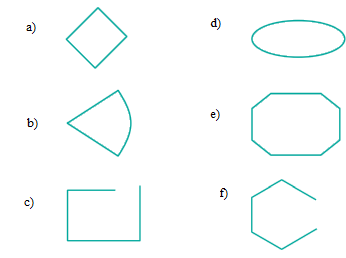
\includegraphics[width=1.7in,height=1.26763in]{./imgSAEB_8_MAT/media/image7.png}
\end{figure}

\reduline{ Somente as alternativas A e E.}

\num{3} Classifique os polígonos abaixo em convexos e não convexos.

\begin{figure}[H]
\centering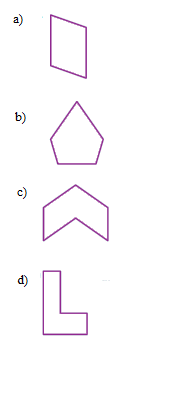
\includegraphics[width=1.16236in,height=2.36667in]{./imgSAEB_8_MAT/media/image8.png}
\end{figure}

\reduline{ a) Convexo.\hfill}
\reduline{ b) Convexo.\hfill}
\reduline{ c) Não convexo.\hfill}
\reduline{ d) Não convexo.\hfill}

\num{2} Utilizando a fórmula d = \frac{n(n - 3)}{2}, calcule o número
de diagonais de um polígono de
\item 5 lados.
\item 9 lados.
\item 10 lados.
\item 15 lados.
\item 20 lados.

++R:
\item d = \frac{5(5 - 3)}{2} = (\frac{25 - 15}{2})
\frac{10}{2} = 5 diagonais
\item d = \frac{9(9 - 3)}{2} = (\frac{81 - 27}{2}
\frac{54}{2}) = 27 diagonais
\item d = \frac{10(10 - 3)}{2} = \frac{100 - 30}{2}
\frac{70}{2} = 35 diagonais
\item d = \frac{15(15 - 3)}{2} = (\frac{225 - 45}{2})
\frac{180}{2}) = 90 diagonais
\item d = \frac{20(20 - 3)}{2} = \frac{400 - 60}{2}
\frac{340}{2} = 170 diagonais

\num{3} Utilizando a fórmula Si = (n - 2) . 180°, calcule a soma dos ângulos
internos dos polígonos abaixo.
\item Quadrilátero.
\item Pentágono.
\item Eneágono.
\item Icoságono.
\item Dodecágono.

++R:
\item Si = (4-2) . 180°
Si = 2 \cdot 180°
Si = 360

\item Si = (5-2) . 180°
Si = 3 \cdot 180
Si = 540

\item Si = (9-2) . 180°
Si = 7 \cdot 180°
Si = 1260

\item Si = (20-2) . 180°
Si = 18 \cdot 180°
Si = 3240

\item Si = (12-2) . 180°
Si = 10 \cdot 180
Si = 1800

\num{4} Utilizando a fórmula Si = (n-2) . 180°, calcule o número de lados dos
polígonos cuja soma dos ângulos internos é:
\item 1080°
\item 1980°
\item 2340°
\item 1800°

++R:
\item 1080 = (n-2) . 180°
(\frac{1080}{180})= n - 2
6 = n - 2
n = 8

\item 1980 = (n-2) . 180°
(\frac{1980}{180}) = n - 2
11 = n - 2
n = 13

\item 2340 = (n-2) . 180°
(\frac{2340}{180}) = n - 2
13 = n - 2
n = 15

\item 1800 = (n-2) . 180°
(\frac{1800}{180}) = n - 2
10 = n - 2
n = 12

\num{5} Considere o paralelogramo a seguir. Nele, estão expressas as medidas
de dois ângulos opostos. Quais são as medidas dos quatro ângulos desse
paralelogramo?

\begin{figure}[H]
\centering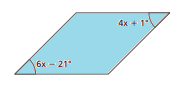
\includegraphics[width=1.82292in,height=0.95833in]{./imgSAEB_8_MAT/media/image9.png}
\end{figure}

\reduline{ 4x + 1 = 6x - 21\hfill}
\reduline{ -2x = -22\hfill}
\reduline{ x = 11\hfill}

Substituindo x = 11 nas duas equações, temos que:

4 \cdot 11 + 1 = 45°

6 \cdot 11 - 21 = 45°

Como a soma dos ângulos internos de um paralelogramo é 360°,

45° + 45° - 360° = 270°

270° \div 2 = 135°

Temos então que o paralelogramo possui 2 ângulos de 45° e 2 ângulos de
135°.

\num{6} Calcule o valor de x e y na figura indicada.

\begin{figure}[H]
\centering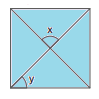
\includegraphics[width=1.03125in,height=1.03125in]{./imgSAEB_8_MAT/media/image10.png}
\end{figure}

\reduline{ Relembrando que a soma dos ângulos internos de um triangulo é = 180° e\hfill}
\reduline{ que a soma dos ângulos internos de um paralelogramo é igual a 360°,\hfill}
\reduline{ temos que y=45° e x = 90°.\hfill}

\num{7} Determine a medida x no paralelogramo da figura a seguir.

\begin{figure}[H]
\centering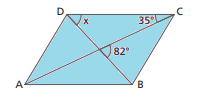
\includegraphics[width=2.05208in,height=1.09375in]{./imgSAEB_8_MAT/media/image11.png}
\end{figure}

\reduline{ Por método de observação, temos que o ângulo no ponto B é:\hfill}
\reduline{ 82°+ 35° - 180° = 63°\hfill}
\reduline{ Formando um triangulo BCD, temos que\hfill}
\reduline{ 70° + 63° - 180° = 47°\hfill}

\num{8} Analise a circunferência de centro A representada a seguir e
classifique em raio, diâmetro ou corda o segmento de reta:

\begin{figure}[H]
\centering
\includegraphics[width=2.98681in,height=2.57292in]{./imgSAEB_8_MAT/media/image12.png}
\end{figure}
\item GA
\item DC
\item EF
\item GH
\item AB
\item DA
\item HI
\item AC
\item AH

++R:
\item raio
\item diâmetro; corda
\item corda
\item diâmetro; corda
\item raio
\item raio
\item corda
\item raio
\item raio

\section{Treino}

\num{1} Alfredo desenhou, em uma madeira, um eneágono regular cujo perímetro
era de 117 cm. Qual é a medida de cada lado dessa figura?
\item 13 cm
\item 11,7 cm
\item 16,71 cm
\item 23,4 cm

SAEB: Construir/desenhar figuras geométricas planas ou espaciais que
satisfaçam condições dadas.

BNCC: EF08MA18 -- Reconhecer e construir figuras obtidas por composições
de transformações geométricas (translação, reflexão e rotação), com o
uso de instrumentos de desenho ou de softwares de geometria dinâmica.

A: Correta, pois 117 \div 9 = 13 cm de lado tem essa figura.

B: Incorreta, pois o aluno poderia chegar a essa conclusão caso
considerasse que o eneágono regular possui 10 lados e não 9.

c: Incorreta, pois o aluno poderia chegar a essa conclusão caso
considerasse que o eneágono regular possui 7 lados e não 9.

D: Incorreta, pois o aluno poderia chegar a essa conclusão caso
considerasse que o eneágono regular possui 5 lados e não 9.

\num{2} O~centro do campo~de futebol é marcado com um ponto. Ao redor,
traçamos um~círculo~com raio de 9,15 metros. Com essas informações em
mente, qual é a área do círculo central de um campo de futebol,
aproximadamente?

Considere (\pi = 3)
\item 54,1 m^2
\item 27,41 m^2
\item 251 m^2
\item 27,66 m^2

SAEB: Construir/desenhar figuras geométricas planas ou espaciais que
satisfaçam condições dadas.

BNCC: EF08MA18 -- Reconhecer e construir figuras obtidas por composições
de transformações geométricas (translação, reflexão e rotação), com o
uso de instrumentos de desenho ou de softwares de geometria dinâmica.

A: Incorreta, poiso aluno chegaria a esse valor caso confundisse a
fórmula da área do círculo com a fórmula do perímetro do círculo.

B: Incorreta, pois o aluno chegaria a essa conclusão caso se esquecesse
do termo quadrático da expressão.

C: Correta, pois

(A = \pi r^{2})

A = 3 \cdot 9,15^2

A= 3. 83,7225

A= 251 m^2

D: Incorreta, pois o aluno chegaria a esse resultado caso dividisse a
expressão no final da fórmula ao invés de multiplicar.

\num{3} Iolanda faz peças com tecidos. Uma das peças mais vendidas é um porta
joias com formato de um hexágono regular de 5 cm de lado com a borda
revestida com uma fita. Quantos centímetros de fita, no mínimo, Iolanda
precisa para confeccionar 20 porta joias?
\item 6 metros
\item 600 metros
\item 5 metros
\item 4 metros

SAEB: Construir/desenhar figuras geométricas planas ou espaciais que
satisfaçam condições dadas.

BNCC: EF08MA18 -- Reconhecer e construir figuras obtidas por composições
de transformações geométricas (translação, reflexão e rotação), com o
uso de instrumentos de desenho ou de softwares de geometria dinâmica.

A: Correta, pois:

Hexágono regular = 6 lados

30 cm por porta joias

20 \cdot 30 cm = 600 cm de fita ou 6 metros de fita

B: Incorreta, pois o aluno pode chegar a esse valor confundindo cm com
metros.

C: Incorreta, pois o aluno pode chegar a esse valor considerando que um
hexágono regular contenha 5 lados.

D: Incorreta, pois o aluno pode chegar a esse valor considerando que um
hexágono regular contenha 4 lados.


\chapter{Triângulos}

\section{Habilidades do SAEB}

\begin{itemize}
\item Identificar propriedades e relações existentes
entre os elementos de um triângulo (condição de existência, relações de
ordem entre as medidas dos lados e as medidas dos ângulos internos, soma
dos ângulos internos, determinação da medida de um ângulo interno ou
externo).
\item
  Classificar triângulos ou quadriláteros em relação aos lados ou aos
  ângulos internos.
\item
  Identificar retas ou segmentos de retas concorrentes, paralelos ou
  perpendiculares.
\item
  Identificar relações entre ângulos formados por retas paralelas
  cortadas por uma transversal.
\item
  Resolver problemas que envolvam relações entre ângulos formados por
  retas paralelas cortadas por uma transversal, ângulos internos ou
  externos de polígonos ou cevianas (altura, bissetriz, mediana,
  mediatriz) de polígonos.
\item
  Resolver problemas que envolvam relações métricas do triângulo
  retângulo, incluindo o teorema de Pitágoras.
\item
  Resolver problemas que envolvam polígonos semelhantes.
\item
  Resolver problemas que envolvam aplicação das relações de
  proporcionalidade abrangendo retas paralelas cortadas por
  transversais.
\item
  Determinar o ponto médio de um segmento de reta ou a distância entre
  dois pontos quaisquer, dadas as coordenadas desses pontos no plano
  cartesiano.
\end{itemize}

\subsection{Habilidade da BNCC}

\begin{itemize}
\item EF08MA14.
\end{itemize}

Triângulos

Elementos de um triângulo

\begin{itemize}
\item
  Vértices
\item
  Lados
\item
  Ângulos internos
\item
  Ângulos externos
\end{itemize}

Classificação de triângulos

Classificamos os triângulos em relação às medidas de seus lados ou às
medidas de seus ângulos internos. Em relação às medidas dos lados, um
triângulo é classificado como:

\begin{itemize}
\item
  Equilátero: Quando os três lados têm medidas iguais.
\item
  Isósceles: Quando dois lados têm medidas iguais.
\item
  Escaleno: Quando os três lados têm medidas diferentes.
\end{itemize}

Em relação às medidas dos ângulos, um triângulo é classificado como:

\begin{itemize}
\item
  Acutângulo: Quando os três ângulos internos são agudos (menores que
  90º)
\item
  Retângulo: Quando um dos ângulos internos é reto (medida igual a 90º).
\item
  Obtusângulo: Quando um dos ângulos internos é obtuso (a medida é maior
  que 90º e menor que 180º).
\end{itemize}

Bissetriz de um triângulo

A bissetriz de um triângulo é o segmento de reta que une um de seus
vértices ao seu respectivo lado oposto, dividindo o ângulo desse vértice
em dois ângulos de mesma medida.

Mediatriz

A mediatriz de um dos lados de um triângulo é a reta perpendicular a
esse lado que passa pelo seu ponto médio.

Todo triângulo possui três mediatrizes que se encontram em um único
ponto denominado circuncentro.

Triângulos congruentes

Triângulos congruentes são triângulos que possuem os mesmos comprimentos
de lados e os mesmos valores de ângulos

\section{Atividades}

\num{1} Observe a figura abaixo e indique o que se pede em cada alternativa.

\begin{figure}[H]
\centering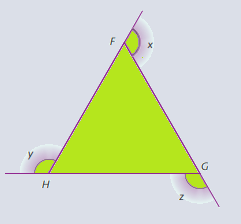
\includegraphics[width=1.88333in,height=1.75048in]{./imgSAEB_8_MAT/media/image13.png}
\end{figure}
\item os vértices do triângulo;
\item os lados do triângulo;
\item os ângulos internos do triângulo;
\item os ângulos externos do triângulo;
\item o lado oposto ao ângulo F

++R:
\item F, G e H
\item FH, FG e HG
\item F, G e H
\item x, y e z
\item HG

\num{2} No triângulo representado a seguir, AD é a bissetriz em relação a
BÂC. Determine o valor de x, em graus.

\begin{figure}[H]
\centering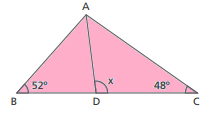
\includegraphics[width=2.20833in,height=1.1875in]{./imgSAEB_8_MAT/media/image14.png}
\end{figure}

\reduline{ Considerando a soma dos ângulos internos, temos que:\hfill}

52 + 48 = 100

Logo, o ângulo BÂC = 80,° e o valor de sua bissetriz é 40°.

Assim, o ângulo x possui:

40 + 48 = 88

180 - 88 = 92°.

\num{3} Em cada caso descrito, analise se é possível construir um triângulo
com lado BC de 5 cm e com as medidas dos ângulos indicadas.
\item medida do ângulo (B)= 110° e medida do ângulo (C) = 50°
\item medida do ângulo (B) = 110° e medida do ângulo (C)= 70°
\item medida do ângulo (B) = 110° e medida do ângulo (C) = 90°

++R:
\item onsiderando que a soma dos ângulos internos do triângulo deve ser 180,
chegamos à conclusão de que é possível.
\item onsiderando que a soma dos ângulos internos do triângulo deve ser 180,
chegamos à conclusão de que não é possível.
\item onsiderando que a soma dos ângulos internos do triângulo deve ser 180,
chegamos à conclusão de que não é possível.

\num{4} Em cada triângulo representado a seguir, onde foram traçadas algumas
retas, identifique se o ponto O é circuncentro, incentro, baricentro ou
ortocentro.
\item
\begin{figure}[H]
\centering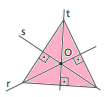
\includegraphics[width=1.14583in,height=1.01042in]{./imgSAEB_8_MAT/media/image15.png}
\end{figure}
\item
\begin{figure}[H]
\centering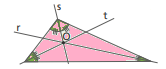
\includegraphics[width=1.72917in,height=0.71875in]{./imgSAEB_8_MAT/media/image16.png}
\end{figure}
\item
\begin{figure}[H]
\centering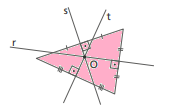
\includegraphics[width=1.84375in,height=1.125in]{./imgSAEB_8_MAT/media/image17.png}
\end{figure}
\item
\begin{figure}[H]
\centering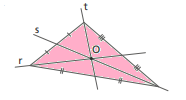
\includegraphics[width=1.9375in,height=1.04167in]{./imgSAEB_8_MAT/media/image18.png}
\end{figure}

++R:
\item Ortocentro
\item Incentro
\item Circuncentro
\item Baricentro

\num{5} Em cada item, verifique se os triângulos são congruentes:
\item
\begin{figure}[H]
\centering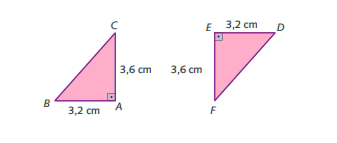
\includegraphics[width=3.51042in,height=1.48958in]{./imgSAEB_8_MAT/media/image19.png}
\end{figure}
\item
\begin{figure}[H]
\centering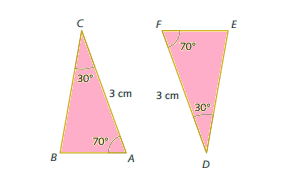
\includegraphics[width=3.16667in,height=2.03958in]{./imgSAEB_8_MAT/media/image20.png}
\end{figure}
\item
\begin{figure}[H]
\centering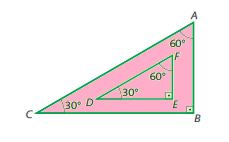
\includegraphics[width=2.38542in,height=1.47917in]{./imgSAEB_8_MAT/media/image21.png}
\end{figure}
\item
\begin{figure}[H]
\centering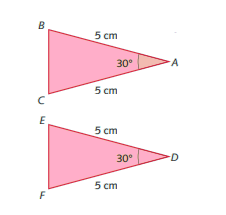
\includegraphics[width=2.35417in,height=2.23958in]{./imgSAEB_8_MAT/media/image22.png}
\end{figure}
\item
\begin{figure}[H]
\centering
\includegraphics[width=2.73958in,height=1.54167in]{./imgSAEB_8_MAT/media/image23.png}
\end{figure}

++R:
\item São congruentes
\item São congruentes
\item Não são congruentes
\item São congruentes
\item São congruentes

\num{6} Calcule, em graus, as medidas dos ângulos dos triângulos abaixo:
\item
\begin{figure}[H]
\centering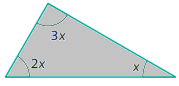
\includegraphics[width=1.86458in,height=0.89583in]{./imgSAEB_8_MAT/media/image24.png}
\end{figure}
\item
\begin{figure}[H]
\centering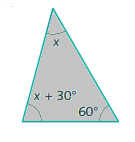
\includegraphics[width=1.40625in,height=1.47917in]{./imgSAEB_8_MAT/media/image25.png}
\end{figure}
\item
\begin{figure}[H]
\centering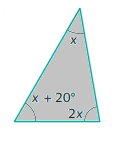
\includegraphics[width=1.30208in,height=1.5625in]{./imgSAEB_8_MAT/media/image26.png}
\end{figure}
\item
\begin{figure}[H]
\centering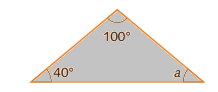
\includegraphics[width=2.33333in,height=0.95833in]{./imgSAEB_8_MAT/media/image27.png}
\end{figure}
\item
\begin{figure}[H]
\centering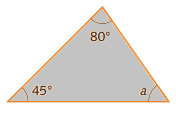
\includegraphics[width=1.83333in,height=1.1875in]{./imgSAEB_8_MAT/media/image28.png}
\end{figure}
\item
\begin{figure}[H]
\centering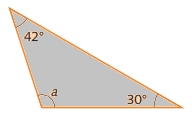
\includegraphics[width=2in,height=1.30208in]{./imgSAEB_8_MAT/media/image29.png}
\end{figure}


\reduline{ a)  3x + 2x + x = 180; 6x = 180; X = 30. Logo, os respectivos ângulos são 30°,60° e 90°.}
\reduline{ b) x + x + 30 + 60 = 180; 2x + 90 = 180; 2x = 90; X = 45}
\reduline{ Logo, os ângulos são 45°, 75° e 60°.}
\reduline{ c) x + x + 20 + 2x = 180; 4x + 20 = 180; 4x = 160; x = 40}
\reduline{ Logo, os ângulos são respectivamente 40°, 60° e 80°}
\reduline{ d) a = 40°; e) a = 55° f) a = 108°}

\num{7} determine as medidas do ângulo complementar e do ângulo suplementar
de cada ilustração a seguir:

\begin{figure}[H]
\centering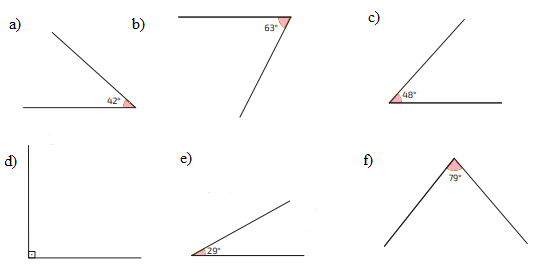
\includegraphics[width=4.81667in,height=2.48373in]{./imgSAEB_8_MAT/media/image30.png}
\end{figure}

\reduline{ 48° e 138°; 27° e 117°; 42° e 132°; 0° e 90°; 61° e 151°; 11° e 101°.\hfill}

\num{8} Ao folear um livro de engenharia de seu pai, Marcos se deparou com a
seguinte imagem:

\begin{figure}[H]
\centering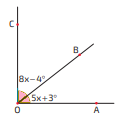
\includegraphics[width=1.47134in,height=1.42708in]{./imgSAEB_8_MAT/media/image31.png}
\end{figure}

Para encontrar o valor de x, quais os passos Enzo deve tomar?

\reduline{ Observar que o ângulo destacado é igual a 90°.\hfill}
\reduline{ Montar a equação da seguinte forma:\hfill}
\reduline{ 8x - 4 + 5x + 3 = 90\hfill}
\reduline{ 13x - 1 = 90\hfill}
\reduline{ 13x = 91\hfill}
\reduline{ x = 7\hfill}

\num{9} Calcule as medidas do ângulos destacados abaixo, considerando que as
linhas em verde traçam a bissetriz de cada ângulo.

\begin{figure}[H]
\centering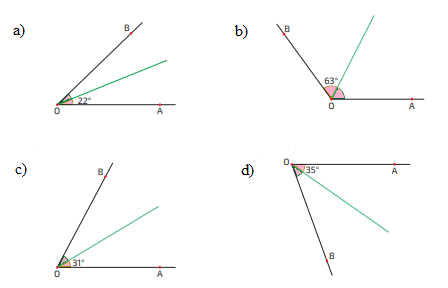
\includegraphics[width=4.66667in,height=3in]{./imgSAEB_8_MAT/media/image32.png}
\end{figure}

\reduline{ 44°, 126°, 62° e 70°.\hfill}

\num{10} Calcule o valor de x nas figuras abaixo.
\item
\begin{figure}[H]
\centering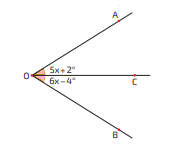
\includegraphics[width=1.91667in,height=1.6875in]{./imgSAEB_8_MAT/media/image33.png}
\end{figure}
\item
\begin{figure}[H]
\centering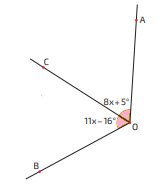
\includegraphics[width=1.80208in,height=2.02917in]{./imgSAEB_8_MAT/media/image34.png}
\end{figure}

++R:
\item

5x + 2 = 6x - 4

-x = -6

X = 6
\item

11x - 16 = 8x + 5

3x = 21

X = 7

\section{Treino}

\num{1} Denomina-se incentro o ponto comum
\item às alturas do triângulo;
\item às mediatrizes dos lados do triângulo;
\item às medianas do triângulo;
\item às bissetrizes do triângulo.

SAEB: Resolver problemas que envolvam relações entre ângulos formados
por retas paralelas cortadas por uma transversal, ângulos internos ou
externos de polígonos ou cevianas (altura, bissetriz, mediana,
mediatriz) de polígonos.

BNCC: EF08MA14 -- Demonstrar propriedades de quadriláteros por meio da
identificação da congruência de triângulos.

A: Incorreta, pois essa definição de incentro está errada.

B: Incorreta, pois essa definição de incentro está errada.

C: Incorreta, pois essa definição de incentro está errada.

D: Correta, pois as bissetrizes do triângulo correspondem ao incentro.

\num{2} O triângulo ABC é um triângulo retângulo em A e isósceles. O ponto O
é o seu circuncentro, ou seja, é o centro da circunferência circunscrita
ao triângulo. Se a altura relativa à hipotenusa BC mede 9,3~cm, qual é a
medida da hipotenusa?

\begin{figure}[H]
\centering
\includegraphics[width=2.5625in,height=2.02083in]{./imgSAEB_8_MAT/media/image35.png}
\end{figure}
\item 9,3

\begin{enumerate}
\def\labelenumi{\alph{enumi})}
\setcounter{enumi}{1}
\tightlist
\item
  18,2
\end{enumerate}
\item 18,6
\item 18,8

SAEB: Resolver problemas que envolvam relações entre ângulos formados
por retas paralelas cortadas por uma transversal, ângulos internos ou
externos de polígonos ou cevianas (altura, bissetriz, mediana,
mediatriz) de polígonos.

BNCC: EF08MA14 -- Demonstrar propriedades de quadriláteros por meio da
identificação da congruência de triângulos.

A: Incorreta, pois esse seria o valor relativo, e não a medida final.

B: Incorreta, pois houve um erro na multiplicação.

C: Correta, pois, se a altura relativa à hipotenusa BC mede 9,3~cm, a
medida da hipotenusa será 18,6.

D: Incorreta, pois o aluno chegará a essa conclusão ao errar o cálculo
de multiplicação dos termos destacados no enunciado.

\num{3} Qual é o perímetro de um triângulo com lados cujas medidas são 6 cm,
7 cm e 8 cm?
\item 19 cm
\item 20 cm
\item 21 cm \rosa{-- X}
\item 22cm



SAEB: Identificar propriedades e relações existentes entre os elementos
de um triângulo (condição de existência, relações de ordem entre as
medidas dos lados e as medidas dos ângulos internos, soma dos ângulos
internos, determinação da medida de um ângulo interno ou externo)

BNCC: EF08MA14 -- Demonstrar propriedades de quadriláteros por meio da
identificação da congruência de triângulos.

A: Incorreta, pois o aluno chegará a essa conclusão se, durante o
cálculo da soma dos lados do triangulo, encontrar 2 números a menos.

B: Incorreta, pois o aluno chegará a essa conclusão se, durante o
cálculo da soma dos lados do triangulo, encontrar 1 número a menos.

C: Correta, pois:

Perímetro = soma dos lados, logo 6 + 7 + 8 = 21 cm

D: Incorreta, pois o aluno chegará a essa conclusão se, durante o
cálculo da soma dos lados do triangulo, encontrar 1 número a mais.


\chapter{Representações
espaciais}

\begin{itemize}
\tightlist
\item
  Descrever ou esboçar deslocamento de pessoas e/ou de objetos em
  representações bidimensionais (mapas, croquis etc.), plantas de
  ambientes ou vistas, de acordo com condições dadas.
\end{itemize}

Mapas

Um mapa é uma representação gráfica ou diagrama de uma área geográfica
específica, seja ela uma região, um país, um continente ou até mesmo o
mundo inteiro. Ele é projetado para mostrar a localização relativa de
diferentes elementos geográficos, como cidades, estradas, rios,
montanhas e outros recursos naturais e artificiais.

Os mapas podem ser apresentados em diferentes projeções, que são métodos
de representação tridimensional da Terra em uma superfície
bidimensional. As projeções ajudam a minimizar distorções e deformações
causadas pela transferência de uma esfera para um plano.

Croquis

Um croqui é um tipo de representação gráfica ou esboço rápido e informal
que visa capturar a essência visual ou a forma básica de algo, como um
objeto, um local ou uma ideia. É geralmente um desenho simples,
esquemático e sem muitos detalhes, que serve como um registro visual
rápido e simplificado.

Os croquis são frequentemente usados em diversas áreas, como
arquitetura, design de interiores, design de moda, planejamento urbano,
desenho industrial, arte e até mesmo em anotações pessoais. Eles são uma
maneira rápida e eficiente de visualizar e comunicar ideias
preliminares, conceitos ou esboços iniciais.

Deslocamento

O deslocamento pode ser considerado a distância percorrida por um objeto
ou alguém durante um período de tempo. Essa distância pode ser
representada pela fórmula:

Distância = Velocidade média X tempo

\section{Atividades}

\num{1} Paulo está pretendendo fazer uma longa viagem para visitar seus pais.

\begin{figure}[H]
\centering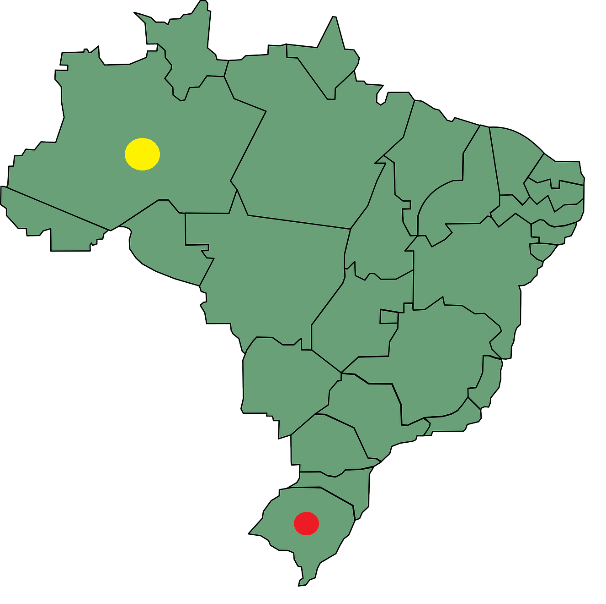
\includegraphics[width=2.73952in,height=2.725in]{./imgSAEB_8_MAT/media/image36.png}
\end{figure}

Disponível em:
\url{https://pixabay.com/pt/vectors/brasil-mapa-am\%c3\%a9rica-do-sul-estados-23553/}.
Acesso em: 23 maio 2023.

Considerando que a casa de Paulo está demarcada com a esfera vermelha e
a casa de seus pais com a esfera amarela, qual é o número mínimo de
estados que Paulo vai ter que atravessar para ver seus pais?

\reduline{ Paulo atravessará, no mínimo, 4 estados até chegar à casa de seus}
pais.

\num{2} A circunferência da terra possui 40.075~km de extensão. Suponhamos
que Júlio queira dar uma volta ao mundo em 80 dias com o seu barco. Qual
deslocamento diário aproximado que deverá percorrer para cumprir seu
objetivo?

\reduline{ Considerando que a terra possui 40.075 km de extensão e a viagem deverá\hfill}
\reduline{ durar, no máximo, 80 dias:\hfill}
\reduline{ 40.075 km \div 80 dias = aproximadamente 501 km por dia.\hfill}

\num{3} Francisco estava em casa e resolveu convidar sua namorada para jantar
fora. Para facilitar o deslocamento, ele encaminhou um mapa da
trajetória.

\begin{figure}[H]
\centering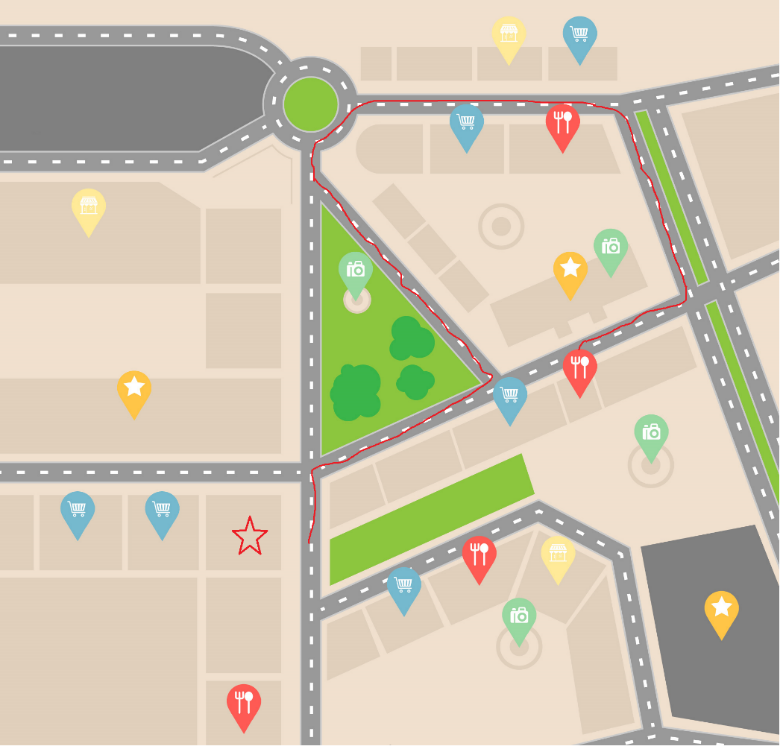
\includegraphics[width=3.55in,height=3.406in]{./imgSAEB_8_MAT/media/image37.png}
\end{figure}

Disponível em:
\url{https://br.freepik.com/vetores-gratis/mapa-cidade-apartamento-desenho_1107608.htm\#query=mapas\&position=6\&from_view=search\&track=sph}.
Acesso em: 23 maio 2023. Adaptado.

Caso ela não consiga abrir a imagem, como ele poderia descrever o
caminho?

\reduline{ Ao sair da Residência de Francisco, pegue a primeira rua à direita,}
\reduline{ depois vire à esquerda, depois entre }
\reduline{ na rotatória e saia na primeira}
\reduline{ saída e siga em frente, depois vire à direita na avenida e finalment vire à direita.}

\num{4} Em uma tarde de domingo, João estava entediado e resolveu dar um
passeio na roda gigante de sua cidade.

\begin{figure}[H]
\centering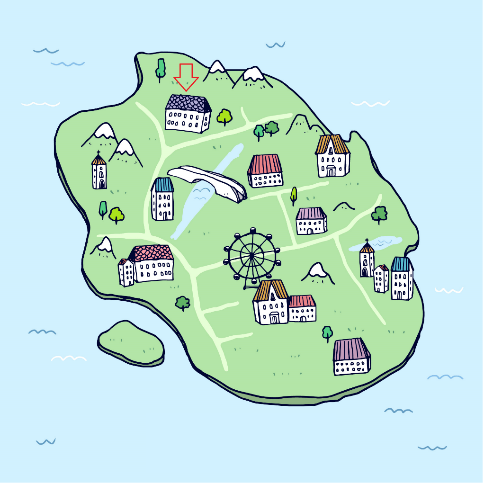
\includegraphics[width=2.2in,height=2.2in]{./imgSAEB_8_MAT/media/image38.png}
\end{figure}

%Disponível em:
%\url{https://br.freepik.com/vetores-gratis/mao-desenhado-cidade-mapa-ferris-roda_1106040.htm\#query=mapa\%20feito\%20a\%20m\%C3\%A3o\&position=6\&from_view=search\&track=ais}.
%Acesso em 23 maio 2023.

Considerando que João mora na casa marcada com a seta no mapa, qual
trajeto até a roda gigante pode ser traçado?

\reduline{ João pode chegar até a roda gigante por dois caminhos. O primeiro,\hfill}
\reduline{ pegando a estrada à direita da sua casa e seguindo nela até virar à\hfill}
\reduline{ esquerda na estrada da roda gigante.\hfill}
\reduline{ O segundo, passando pela ponte à direita de sua casa, atravessando pela\hfill}
\reduline{ ponte e seguindo na estrada, virando à direita após atravessar a ponte e\hfill}
\reduline{ finalmente virar à esquerda.\hfill}

\num{5} Considerando que a distância entre a terra e a lua é de 384.400~km,
qual é o deslocamento total percorrido por um astronauta que pisa no
satélite natural e retorna ao planeta?

\reduline{ 384.400 na ida + 384.400 na volta = deslocamento total = 768.400 km.}

\num{6} Lia está fazendo um test drive com um carro de uma concessionária. Ao
sair, recebeu as seguintes dicas do GPS:

Siga em frente 100m

Vire à esquerda 200m

Vire à esquerda 200 m

Vire à esquerda 200 m

Vire à esquerda 100 m

Ao receber essas informações, pode-se afirmar que aconteceu o quê?

\reduline{ Lia voltou à concessionária.\hfill}

\num{7} Marcelo e amigos estavam indo para praia. No meio do caminho,
perceberam que esqueceram a bagagem em casa. Assim, resolveram voltar
para pegá-la e, enfim, seguir viagem.

Considerando que a distância entre a casa e a praia seja de 300 km, qual
é o deslocamento total de Marcelo e seus amigos até chegarem à praia?

\reduline{ Considerando que já estavam na metade do caminho, percorreram 150 km + a\hfill}
\reduline{ viagem completa de 300km, ou seja, temos que 150 km + 300 km = 450 km.\hfill}

\num{8} Cléber é motorista de ônibus de uma metrópole brasileira. Sua linha
anda por 3 bairros diferentes em um percurso total de 32 km. Sabendo que
Cléber trabalha das 6 horas da manhã até as 16 horas e realiza esse
percurso 4 vezes, qual é o descolamento diário de Cléber no trabalho?

\reduline{ 32 km cada percurso, Cléber realiza o percurso 4 vezes por dia; logo, temos que}

4 \cdot 32 km = 128 km por dia.

\num{9} Marina vai ao trabalho de carro de segunda a sexta. A distância da
casa de marina até seu trabalho é de 12 km. Sabendo que seu carro gasta
0,50 centavos de gasolina a cada 1 km, qual é o valor total que Marina
gasta com combustível durante a semana?

\reduline{ 12 km para ir e 12 km para voltar = 24 km diários}

Logo, se a cada 1 km Marina gasta 0,50 centavos, temos que, em 24 km,
ela gasta R\$\,12,00.

Contando 5 dias trabalhados na semana, 12 \cdot 5 = R\$\,60,00 por semana.

\num{10} Em um livro infantil, um menino sai vagando pelo espaço, de planeta
em planeta, caçando novas aventuras. Considerando que, durante a
história do livro, ele tenha visitado 8 planetas, e que a distância
entre cada planeta seja de (10^5) km, qual foi o deslocamento que o
menino da história realizou?

\reduline{ Considerando 8 planetas, temos que:\hfill}
\reduline{ 8 x (10^5)\hfill}
\reduline{ 8 \cdot 100.000 = 800.000 km\hfill}

\section{Treino}

\num{1} Um jogador de Futebol corre em média 8 km por partida. Considerando
que um campeonato tenha 38 rodadas e que esse jogador jogue todas as
partidas, qual é deslocamento total durante o campeonato?
\item 8 km por campeonato
\item 38 km por campeonato
\item 30,4 km por campeonato
\item 304 km por campeonato

Habilidade SAEB: Descrever ou esboçar deslocamento de pessoas e/ou de
objetos em representações bidimensionais (mapas, croquis etc.), plantas
de ambientes ou vistas, de acordo com condições dadas.

A: Incorreta, pois, ao considerar que o enunciado pede o valor de km por
partida, o aluno pode chegar a essa conclusão.

B: Incorreta, pois ao considerar a quantidade de rodadas ao invés da
quantidade de km percorridos, o aluno pode chegar a esse valor.

C: Incorreta, pois, ao deslocar erroneamente uma vírgula para a
esquerda, o aluno pode chegar a esse resultado.

D: Correta, pois

8 km x 38 partidas = 304 km por campeonato.

\num{2} A velocidade de uma baleia azul pode chegar a 50 km/h. Considerando
que uma baleia esteja a navegar pelo mar em sua velocidade máxima, e que
nade por 8 horas ininterruptas, qual é seu deslocamento total?
\item 40 km
\item 4.000 km
\item 400 km
\item 40.000 km

SAEB: Descrever ou esboçar deslocamento de pessoas e/ou de objetos em
representações bidimensionais (mapas, croquis etc.), plantas de
ambientes ou vistas, de acordo com condições dadas.

A: Incorreta, pois esse seria o valor caso o aluno realizasse
incorretamente a multiplicação.

B: Incorreta, pois esse seria o valor caso o aluno realizasse
incorretamente a multiplicação, adicionando um ``zero'' na expressão.

C: Correta pois:

(\frac{50}{x} = \frac{1}{8})

50 \cdot 8 = x

400 km.

D: Incorreta, pois esse seria o valor caso o aluno realizasse
incorretamente a multiplicação, adicionando dois ``zeros'' na expressão.

\num{3} Charles é um botânico de renome e, ao sair para realizar pesquisas em
uma floresta, acabou se perdendo no meio da mata. Ele também esqueceu
seus equipamentos de navegação em seu laboratório, e a única coisa de
que se lembra é que a cidade mais próxima fica ao rumo do pôr sol. Para
chegar à cidade mais próxima, para qual sentido Charles deve andar?
\item Norte
\item Sul
\item Leste
\item Oeste

SAEB: Descrever ou esboçar deslocamento de pessoas e/ou de objetos em
representações bidimensionais (mapas, croquis etc.), plantas de
ambientes ou vistas, de acordo com condições dadas.

A: Incorreta, pois o aluno pode se confundir em relação aos pontos
cardeais.

B: Incorreta, pois o aluno pode se confundir em relação aos pontos
cardeais.

C: Incorreta, pois o aluno pode se confundir em relação aos pontos
cardeais.

D: Correta, pois Charles deve seguir rumo ao Oeste.


\chapter{Introdução à
Estatística}

\section{Habilidades do SAEB}

\begin{itemize}
\item Identificar os indivíduos (universo ou
população-alvo da pesquisa), as variáveis e os tipos de variáveis
(quantitativas ou categóricas) em um conjunto de dados.
\item
  Representar ou associar os dados de uma pesquisa estatística ou de um
  levantamento em listas, tabelas (simples ou de dupla entrada) ou
  gráficos (barras simples ou agrupadas, colunas simples ou agrupadas,
  pictóricos, de linhas, de setores, ou em histograma).
\item
  Inferir a finalidade da realização de uma pesquisa estatística ou de
  um levantamento, dada uma tabela (simples ou de dupla entrada) ou
  gráfico (barras simples ou agrupadas, colunas simples ou agrupadas,
  pictóricos, de linhas, de setores ou em histograma) com os dados dessa
  pesquisa.
\item
  Interpretar o significado das medidas de tendência central (média
  aritmética simples, moda e mediana) ou da amplitude.
\item
  Calcular os valores de medidas de tendência central de uma pesquisa
  estatística (média aritmética simples, moda ou mediana).
\item
  Resolver problemas que envolvam dados estatísticos apresentados em
  tabelas (simples ou de dupla entrada) ou gráficos (barras simples ou
  agrupadas, colunas simples ou agrupadas, pictóricos, de linhas, de
  setores ou em histograma).
\item
  Argumentar ou analisar argumentações/conclusões com base nos dados
  apresentados em tabelas (simples ou de dupla entrada) ou gráficos
  (barras simples ou agrupadas, colunas simples ou agrupadas,
  pictóricos, de linhas, de setores ou em histograma).
\item
  Explicar/descrever os passos para a realização de uma pesquisa
  estatística ou de um levantamento.
\end{itemize}

\subsection{Habilidade da BNCC}

\begin{itemize}
\item EF08MA25.
\end{itemize}

Conceitos básicos da Estatística

A Estatística é uma área da Matemática voltada ao estudo de métodos para
coleta, organização e análise de dados, visando à tomada de decisões.
Realizamos uma pesquisa estatística quando pretendemos estudar alguma
característica de determinado conjunto de elementos. O conjunto de todos
os elementos analisados na pesquisa é denominado população. Quando temos
muitos elementos na população que queremos estudar, podemos selecionar
uma amostra representativa.

População é o conjunto de elementos que queremos pesquisar e que
apresentam alguma característica comum.

Amostra é um subconjunto da população.

Algumas pesquisas exigem a investigação de toda uma população. Esse tipo
de pesquisa é denominada censitária.

Amostra casual simples

A amostra casual simples é caracterizada por um sorteio aleatório. Os
elementos de uma população podem ser enumerados e, em seguida, sorteados
entre uma quantidade estabelecida previamente.

Amostra sistemática

No caso da amostra sistemática, os elementos da população a ser estudada
já se encontram ordenados. Por exemplo: produtos de uma linha de
produção, prontuários médicos, prédios de uma rua etc. Para a seleção
dos elementos que farão parte da amostra, é elaborado um sistema pelo
pesquisador.

Amostra proporcional estratificada

Na amostra estratificada, a população é dividida em subpopulações
denominadas estratos. Esse tipo de amostra é realizado quando outras
características da população devem ser levadas em conta. Por exemplo,
nas pesquisas de intenção de voto para presidente do Brasil, a população
são os eleitores brasileiros, mas a região do país onde eles residem,
seu sexo, sua faixa etária e sua faixa de renda são dados importantes.
Assim, o pesquisador deve selecionar uma amostra aleatória de cada
estrato.

Variáveis

As variáveis são as características que analisadas em uma amostra ou
população. Elas podem assumir valores numéricos e não numéricos, sendo
classificadas em qualitativas e quantitativas.

Organização dos dados

Para organizar os dados obtidos por meio de uma pesquisa, podemos
construir tabelas e gráficos. O tipo de tabela e de gráfico que vamos
utilizar é condicionado pela variável analisada.

Média aritmética

A média aritmética simples de uma série de dados é determinada pela soma
de todos os dados dividida pela quantidade de dados.

Moda

A moda de uma série de dados é determinada pelo valor que apresenta a
maior frequência.

Mediana

A mediana é a medida estatística que divide o conjunto de dados em duas
partes com a mesma quantidade de termos. Enquanto a primeira parte
apresenta valores menores ou iguais a ela, a segunda parte é formada por
valores maiores.

\section{Atividades}

\num{1} Leia o gráfico a seguir e responda.

\begin{figure}[H]
\centering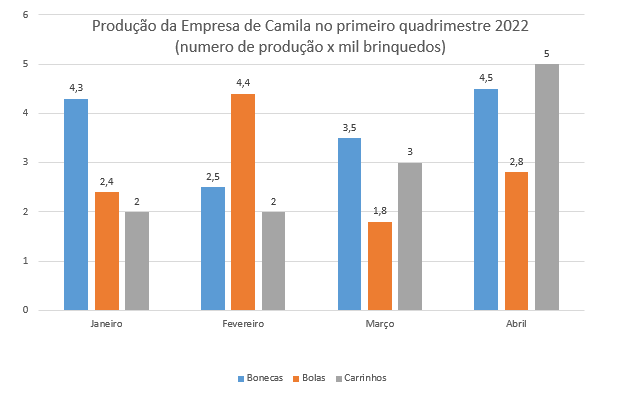
\includegraphics[width=5.90625in,height=3.86458in]{./imgSAEB_8_MAT/media/image39.png}
\end{figure}
\item O mês em que houve a maior quantidade de brinquedos produzidos foi:
\item O mês em que houve a menor quantidade de produção:
\item O brinquedo mais produzido foi:
\item O brinquedo menos foi produzido foi:
\item Quantos brinquedos ao total a empresa de Camila produziu no primeiro
quadrimestre de 2022?

++R:
\item Abril
\item Março
\item Os brinquedos mais produzidos foram as Bonecas
\item Os brinquedos menos reproduzidos foram as bolas
\item Realizando a soma dos dados do gráfico, obtemos que a empresa de
Camila fabricou um total de 38.400 brinquedos.

\num{2} Ronaldo resolveu colocar em um gráfico todos os custos mensais de sua
casa.

\begin{figure}[H]
\centering
\includegraphics[width=5.30833in,height=3.41384in]{./imgSAEB_8_MAT/media/image40.png}
\end{figure}

Ao analisar o gráfico, responda.
\item Ronaldo comprou um ar-condicionado que consome muita energia. Qual
foi o mês da compra?
\item A filha de Ronaldo contratou um plano adicional de internet. Qual foi
o mês da aquisição?
\item Qual conta nunca apresentou uma grande alta de valor?
\item Em que mês Ronaldo pagou o menor valor de contas na sua casa?

++R:
\item Entre o mês de janeiro e fevereiro.
\item No mês de maio.
\item A conta de Água.
\item Janeiro.

\num{3} Poliana está passando por uma reeducação financeira e começou a
dividir seus gastos de forma que ainda sobre um dinheiro para
aproveitar.

\begin{figure}[H]
\centering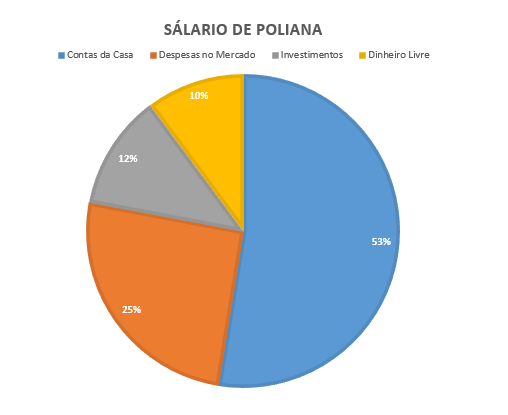
\includegraphics[width=3.65in,height=2.98179in]{./imgSAEB_8_MAT/media/image41.png}
\end{figure}

Considerando que o salário mensal de Poliana é R\$\,3.000,00, responda:
\item O valor destinado mensalmente para as contas da casa.
\item O valor destinado mensalmente para despesas no mercado.
\item O valor destinado mensalmente para investimentos.
\item Poliana quer comprar um carro novo no valor de R\$\,30.000,00. Se
Poliana utilizar a parte de investimentos do seu salário, quantos meses
demorará até comprar o carro?.

++R:
\item 3.000 \cdot 0,53 = R\$\,1.590,00
\item 3.000 \cdot 0,25 = R\$\,750,00
\item 3.000 \cdot 0,12 = R\$\,360,00
\item 30.000 \div 360 = 84 meses

\num{4} Um professor realizou uma pesquisa com sua turma de matemática para
identificar a altura dos estudantes. Os dados coletados foram os
seguintes (em centímetros):

150, 165, 160, 155, 170, 160, 160, 165, 155, 165

Calcule a média aritmética simples, a moda e a mediana das alturas dos
estudantes.

\reduline{ Média aritmética simples:\hfill}
\reduline{ (150 + 165 + 160 + 155 + 170 + 160 + 160 + 165 + 155 + 165) / 10 = 159,5 cm\hfill}
\reduline{ Para encontrar a moda, identificamos o valor que mais se repete. Nesse\hfill}
\reduline{ caso, temos duas alturas que se repetem mais vezes, que são 160 cm e 165\hfill}
\reduline{ cm, ambas aparecendo três vezes. Portanto, a moda das alturas dos\hfill}
\reduline{ estudantes é 160 cm e 165 cm.\hfill}
\reduline{ Para encontrar a mediana, ordenamos os valores em ordem crescente.\hfill}
\reduline{ Assim, temos: 150, 155, 155, 160, 160, 160, 165, 165, 165, 170\hfill}
\reduline{ Como temos um número ímpar de dados (10), a mediana será o valor\hfill}
\reduline{ central. Nesse caso, a mediana das alturas dos estudantes é 160 cm.\hfill}

\num{5} Um professor deseja calcular a média aritmética das notas finais de
seus alunos em uma disciplina. Ele possui os seguintes dados das notas
dos alunos: 7, 8, 6, 9, 5, 8, 7, 6.

Calcule a média aritmética simples das notas dos alunos e explique a
resposta.

Resolução:

Para calcular a média aritmética simples das notas dos alunos, devemos
somar todas as notas e dividir pelo número total de alunos.

Passo 1: Somar as notas 7 + 8 + 6 + 9 + 5 + 8 + 7 + 6 = 56

Passo 2: Dividir pelo número total de alunos 56 / 8 = 7

A média aritmética simples das notas dos alunos é igual a 7.

\num{6} Uma empresa está realizando uma pesquisa sobre o nível de satisfação
de seus funcionários. Para isso, foi feito um levantamento com 35
colaboradores dos 300 registrados na empresa. Com base nas informações
anteriores, responda:
\item Qual é a população dessa pesquisa?
\item Qual é a sua amostra?

++R:
\item Os 300 funcionários registrados.
\item 35 funcionários.

\num{7} O quadro mostra algumas notas de matemática de alguns alunos do 8°.
ano.

%Paulo, criar uma tabela com as informações abaixo:

\begin{longtable}[]{@{}lllll@{}}
\toprule
Notas da disciplina Matemática & & & &\tabularnewline
\midrule
\endhead
Alunos & 1° bimestre & 2° bimestre & 3° bimestre & 4°
bimestre\tabularnewline
Adriana & 7 & 6,5 & 9 & 8\tabularnewline
Bruno & 3 & 5 & 6 & 5\tabularnewline
Carla & 9 & 9 & 8 & 9\tabularnewline
José & 10 & 8 & 8 & 8\tabularnewline
Renata & 5 & 4 & 5 & 3\tabularnewline
\bottomrule
\end{longtable}

Sobre as notas, responda:
\item Qual é a média aritmética das notas que Adriana obteve nos 4
bimestres?
\item Qual é a média aritmética das notas que Bruno obteve nos 4 bimestres?
\item Qual é a média aritmética das notas que Carla obteve nos 4 bimestres?
\item Qual é a média aritmética das notas que José obteve nos 4 bimestres?
\item Qual é a média aritmética das notas que Renata obteve nos 4
bimestres?
\item Sabendo que, para ser aprovado na disciplina, a média das notas dos 4
bimestres devem ser maior que 6, quais alunos foram aprovados? Quais
foram reprovados?

++R:
\item

7 + 6,5 + 9 + 8 = 30,5

30,5 \div 4 = 7,625
\item

3 + 5 + 6 + 5 = 19

19:4 = 4,75
\item 9 + 9 + 8 + 9 = 35

35:4 = 8,75
\item

10 + 8 + 8 + 8 = 34

34 \div 4 = 8,5
\item

5 + 4 + 5 + 3 = 17

17 \div 4 = 4,25
\item Bruno e Renata foram reprovados.

\num{8} Dona Catarina, de 82 anos, tem 5 irmãs: Genoveva, de 79 Anos,
Clotilde, de 75, Amélia, de 70, Irene, de 67, e Tereza, de 64. Qual é a
média de idade de todas as irmãs?

\reduline{ 82 + 79 + 75 + 70 + 67 + 64 = 437\hfill}
\reduline{ 437 \div 6 = 72,83\hfill}

% \num{9} Uma professora resolveu fazer uma pesquisa com seus alunos que
% consistia em apenas 1 pergunta: Qual é o número do seu calçado?

% Ela obteve os seguintes dados:

% %Paulo: inserir uma tabela com os dados abaixo. Pesquisa do Número do
% Calçado de cada Aluno do 8° A\\
% ----------------------------------------------------- ---- ---- ----
% ---- ---- 35 38 40 42 38 40 40 38 40 44 40 37 42 37 42 42 40 44 40 35 38
% 40 39 38 35 38 38 38 44 38 39 38 38 37 40 37

% Ao observar esses dados, qual é a moda dos números dos calçados dos
% alunos?

% R: Ao observar o quadro, temos que

% 3 Alunos calçam 35

% 9 alunos calçam 40

% 4 alunos calcam 42

% 2 alunos calçam 39

% 11 alunos calçam 38

% 3 alunos calcam 44

% Logo, por método de observação, temos que a Moda consiste em calçados
% número 38.

\num{9} Um supermercado está realizando uma pesquisa sobre o tempo de espera
dos clientes nas filas dos caixas. Foram registrados os seguintes tempos
de espera em minutos: 3, 5, 2, 4, 6, 3, 5, 4, 2, 3.
Calcule a média aritmética simples do tempo de espera dos clientes e
explique a resposta.

\reduline{ Para calcular a média aritmética simples do tempo de espera dos\hfill}
\reduline{ clientes, devemos somar todos os tempos de espera e dividir pelo número\hfill}
\reduline{ total de observações.\hfill}
\reduline{ Passo 1: Somar os tempos de espera 3 + 5 + 2 + 4 + 6 + 3 + 5 + 4 + 2 + 3 = 37.\hfill}
\reduline{ Passo 2: Dividir pelo número total de observações 37 / 10 = 3,7 minutos.\hfill}

\section{Treino}

\num{1} Em um jogo de basquete, os 5 atletas de um time que iniciaram o jogo
tinham respectivamente 2,01 m, 1,99 m, 2,00 m, 2,02 m e 1,98 m de
altura. Qual é a estatura média dessa equipe titular?
\item 2,02 m
\item 1,98 m
\item 2 m
\item 10 m

SAEB: Calcular os valores de medidas de tendência central de uma
pesquisa estatística (média aritmética simples, moda ou mediana).

BNCC: EF08MA25 -- Obter os valores de medidas de tendência central de
uma pesquisa estatística (média, moda e mediana) com a compreensão de
seus significados e relacioná-los com a dispersão de dados, indicada
pela amplitude.

A: Incorreta, pois o aluno chegaria a esse resultado a partir da maior
altura da equipe.

B: Incorreta, pois o aluno chegaria a esse resultado a partir da menor
altura da equipe.

C: Correta, pois:

Somando a altura dos atletas temos:

2,01 + 1,99 + 2,00 + 2,02 + 1,98 =10

Como são 5 atletas

10 \div 5 = 2 metros de altura é a média

D: Incorreta, pois o aluno chegaria a esse resultado a partir da soma
das alturas da equipe.

\num{2} Um grupo de amigos que frequentam uma academia decidiu compartilhar o
valor de sua última pesagem e chegaram aos seguintes números:

46kg, 44kg, 49kg, 45kg, 44kg, 48kg, 50kg, 42kg

Qual é a mediana do peso em kg desses amigos?
\item 44kg
\item 45,5kg
\item 46 kg
\item 45kg

SAEB: Calcular os valores de medidas de tendência central de uma
pesquisa estatística (média aritmética simples, moda ou mediana).

BNCC: EF08MA25 -- Obter os valores de medidas de tendência central de
uma pesquisa estatística (média, moda e mediana) com a compreensão de
seus significados e relacioná-los com a dispersão de dados, indicada
pela amplitude.

A: Incorreta, pois o aluno chegaria a esse resultado calculando a moda,
chegando a uma conclusão equivocada.

B: Correta, pois:

Considerando que os dois pesos centrais são 46 e 45 kg,

46 + 45 = 91

91 \div 2 = 45,5

C: Incorreta, pois o aluno chegaria a esse resultado calculando a média
aritmética, e não a mediana.

D: Incorreta, pois o aluno chegará a esse resultado não levando em
consideração que, em casos de conteúdos pares, a mediana deve ser a
média entre os dois valores centrais.

\num{3} Maria caminha todos os dias até seu trabalho. Durante uma semana,
resolveu cronometrar o tempo que leva no trajeto:

Segunda-feira: 35 minutos

Terça-feira: 32 minutos

Quarta-feira: 33 minutos

Quinta-feira: 34 minutos

Sexta-feira: 36 minutos

Qual é o tempo médio que Maria gasta até chegar no trabalho?
\item 32 minutos
\item 36 minutos
\item 34 minutos
\item 170 minutos

SAEB: Calcular os valores de medidas de tendência central de uma
pesquisa estatística (média aritmética simples, moda ou mediana).

BNCC: EF08MA25 -- Obter os valores de medidas de tendência central de
uma pesquisa estatística (média, moda e mediana) com a compreensão de
seus significados e relacioná-los com a dispersão de dados, indicada
pela amplitude.

A: Incorreta, pois o aluno chegaria a esse resultado considerando
somente o menor tempo gasto.

B: Incorreta, pois o aluno chegaria a esse resultado considerando
somente o maior tempo gasto.

C: Correta, pois:

Somando o tempo que Maria gastou na semana, temos que:

170 minutos / 5 = média de 34 minutos por dia.

D: Incorreta, pois o aluno chegaria a esse resultado considerando
somente a soma dos tempos.


\chapter{Perímetro, área e
volume}

\section{Habilidades do SAEB}

\begin{itemize}
\item Resolver problemas que envolvam medidas de
grandezas (comprimento, massa, tempo, temperatura, capacidade ou volume)
em que haja conversões entre unidades mais usuais.
\item
  Resolver problemas que envolvam perímetro de figuras planas.
\item
  Resolver problemas que envolvam área de figuras planas.
\item
  Resolver problemas que envolvam volume de prismas retos ou cilindros
  retos.
\end{itemize}

\subsection{Habilidades da BNCC}

\begin{itemize}
\item EF08MA19, EF08MA20, EF08MA21.
\end{itemize}

Área e perímetro de figuras planas

Para calcularmos o perímetro de uma figura plana, basta realizarmos a
soma de todos os lados da figura.

Já para o cálculo da área de figuras planas, temos de saber fórmulas
específicas para cada tipo de forma:

Veja alguns exemplos dessas fórmulas:

Área do quadrado: A = l^2

Área do triângulo retângulo: A = (\frac{b.h}{2})

Área do losango: A = (\frac{\text{D . d}}{2})

Área do circulo: (A = \pi r^{2})

Área de um retângulo: (A = l1 \cdot l2)

Volume de poliedros

Cada poliedro também tem uma fórmula específica para o cálculo de seu
volume. Veja alguns exemplos:

Volume de um cubo: V = l . l . l ou l^3

Volume de um cilindro V = (\Pi) . R^2 . h

Volume de um paralelepípedo: (V = l1 \cdot l2 \cdot l3)

\section{Atividades}

\num{1} Considere o cubo abaixo

\begin{figure}[H]
\centering
\includegraphics[width=1.89583in,height=1.27083in]{./imgSAEB_8_MAT/media/image42.png}
\end{figure}
\item Qual é a medida de perímetro de uma das faces desse cubo?
\item E qual é a medida de área de uma das faces dele?
\item Qual é a medida de volume do cubo?

Deixar o espaço de 2 linhas para resposta em cada item acima.

++R:
\item 4 \cdot 3 = 12 cm
\item 3 \cdot 3 = 9 cm^2
\item 3 \cdot 3 . 3 = 27 cm^3

\num{2} Determine a área de uma região quadrada, sabendo que a medida de
comprimento do lado é de:
\item 8 cm
\item 12 cm
\item 16 m
\item 20 m
\item 34 m
\item 8 mm
\item 10 mm
\item 25 mm

++R:
\item 8 \cdot 8 = 64 cm^2
\item 12 \cdot 12 = 144 cm^2
\item16 \cdot 16= 256 m^2
\item20 \cdot 20 = 400 m^2
\item34 \cdot 34= 1156 m^2
\item 8 \cdot 8 = 64 mm^2
\item 10 \cdot 10 = 100 mm^2
\item 25 \cdot 25 = 625 mm^2

\num{3} Calcule a medida do comprimento do lado de uma região quadrada cuja
área é de:
\item 121 cm^2
\item 169 cm^2
\item 225 cm^2
\item 36 m^2
\item 324 m^2
\item 529 m^2
\item 81 mm^2
\item 729 mm^2

++R:
\item (\sqrt{121}) = 11cm

\begin{enumerate}
\def\labelenumi{\alph{enumi})}
\setcounter{enumi}{1}
\item
  (\sqrt{169}) = 13cm
\item
  (\sqrt{225}) = 15 cm
\item
  (\sqrt{36}) = 6 m
\item
  (\sqrt{324}) = 18 m
\item
  (\sqrt{529}) = 23 m
\item
  (\sqrt{81}) = 9 mm
\item
  (\sqrt{729}) = 27 mm
\end{enumerate}

\num{4} Determine a área de cada figura abaixo.
\item
\begin{figure}[H]
\centering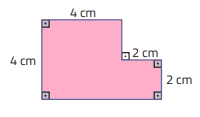
\includegraphics[width=1.65in,height=0.96458in]{./imgSAEB_8_MAT/media/image43.png}
\end{figure}
\item
\begin{figure}[H]
\centering
\includegraphics[width=1.50833in,height=1.28681in]{./imgSAEB_8_MAT/media/image44.png}
\end{figure}

++R:
\item

4 \cdot 4 + 2 \cdot 2 = A

16 + 4 = A

A = 20 cm^2
\item

3 + 3 \cdot 3 = A

18 + 9 = A

A = 27cm^2

\num{5} Para construir uma caixa com a forma de um bloco retangular sem
tampa, Rosangela recortou uma região poligonal de papelão, como esta
figura, e dobrou e colou com fita-crepe. Quantos cm^2 de papelão ela
usou?

\begin{figure}[H]
\centering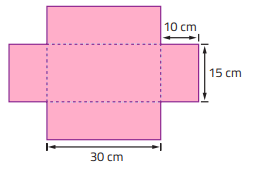
\includegraphics[width=1.98333in,height=1.33255in]{./imgSAEB_8_MAT/media/image45.png}
\end{figure}

\reduline{ Somando todas as áreas das figuras tracejadas, temos que:\hfill}
\reduline{ 10 \cdot 15 + 10 \cdot 15 + 10 \cdot 30 + 10 \cdot 30 + 15 \cdot 30 = A\hfill}
\reduline{ 150 + 150 + 300 + 300 + 450 = A\hfill}
\reduline{ A = 1.350 cm^2\hfill}

\num{6} Determine a área das figuras abaixo
\item
\begin{figure}[H]
\centering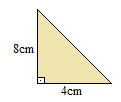
\includegraphics[width=1.26042in,height=1.0625in]{./imgSAEB_8_MAT/media/image46.png}
\end{figure}

\reduline{ A = (\frac{4.8}{2})\hfill}
\reduline{ A = (\frac{32}{2})\hfill}
\reduline{ A = 16m^2\hfill}

\item
\begin{figure}[H]
\centering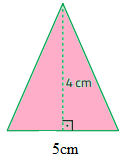
\includegraphics[width=1.39583in,height=1.72917in]{./imgSAEB_8_MAT/media/image47.png}
\end{figure}

\reduline{ A = (\ \frac{\ 2,5.4}{2})\hfill}
\reduline{ A = (\frac{10}{2})\hfill}
\reduline{ A = 5 + 5\hfill}
\reduline{ A = 10cm^2\hfill}
\reduline{ \hfill}
\item
\begin{figure}[H]
\centering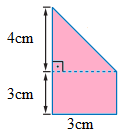
\includegraphics[width=1.375in,height=1.42708in]{./imgSAEB_8_MAT/media/image48.png}
\end{figure}

\reduline{ A = (\frac{12}{2})\hfill}
\reduline{ A = 6\hfill}
\reduline{ 6 + 9 = 15 cm^2\hfill}

\item
\begin{figure}[H]
\centering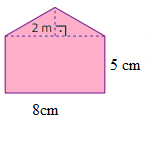
\includegraphics[width=1.59375in,height=1.46875in]{./imgSAEB_8_MAT/media/image49.png}
\end{figure}

\reduline{ A = (\frac{4.2}{2})\hfill}
\reduline{ A = (\frac{8}{2})\hfill}
\reduline{ A = 4\hfill}
\reduline{ 4 + 4 + 8.5 = 48cm^2\hfill}

\num{7} Ao ler a bula de uma medicação, Andreia encontrou a seguinte
informação: ``Cada comprimido possui x mm^3 dentro de sua cápsula''. Como
não conseguiu ler, pois a escrita estava rasurada, Andreia decidiu fazer
suas próprias medidas e obteve:

\begin{figure}[H]
\centering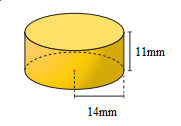
\includegraphics[width=1.88542in,height=1.3125in]{./imgSAEB_8_MAT/media/image50.png}
\end{figure}

Para saber o volume de medicação dentro da cápsula, qual fórmula Andreia deve utilizar?
Considerando-se (\Pi) = 3, qual é o volume da cápsula?

\reduline{ V= (\Pi) . R^2 . h\hfill}
\reduline{ V = 3 \cdot 14 \cdot 11\hfill}
\reduline{ V = 462 mm^3 de medicação.\hfill}

\num{8} Calcule o volume do sólido a seguir.

\begin{figure}[H]
\centering\includegraphics[width=1.94792in,height=0.98958in]{./imgSAEB_8_MAT/media/image51.png}
\end{figure}

\reduline{ V = l . l . l\hfill}
\reduline{ V = 8 \cdot 4 . 3\hfill}
\reduline{ V = 96cm^3\hfill}

\num{9} Calcule o volume do sólido a seguir.
\begin{figure}[H]
\centering\includegraphics[width=2.08333in,height=1in]{./imgSAEB_8_MAT/media/image52.png}
\end{figure}

\reduline{ V = \frac{l . l . l}{2}\hfill}
\reduline{ V = \frac{4 \cdot 12 \cdot 3}{2}\hfill}
\reduline{ V = 72 cm^3\hfill}

\num{10} Calcule o volume do sólido a seguir.
\begin{figure}[H]
\centering\includegraphics[width=1.92708in,height=1.5625in]{./imgSAEB_8_MAT/media/image53.png}
\end{figure}

\reduline{ V_1 = l . l . l\hfill}
\reduline{ V_1 = 20 \cdot 10 \cdot 15\hfill}
\reduline{ V_1 = 3.000\hfill}

\reduline{ V_2 = l . l . l\hfill}
\reduline{ V_2 = 15. 10 .10\hfill}
\reduline{ V_2 = 1.500\hfill}

\reduline{ V_t = 1.500 + 3.000 = 4.500 cm^3\hfill}

\num{11} Marina Resolveu colocar em sua casa uma piscina de 8 metros de
largura, 5 metros de comprimento e 1,5 metros de profundidade. Sabendo
que a companhia de água cobra 0,05 centavos por litro consumido, quantos
reais marina vai gastar para encher completamente essa piscina?

\reduline{ V = 8 \cdot 5 . 1,5 = 60 m^3\hfill}
\reduline{ 60 m^3 = 60 000 litros \cdot 0,20 centavos\hfill}
\reduline{ 12.000 centavos ou R\$\,120,00\hfill}

\num{12} O reservatório de tinta de uma caneta comum tem a forma de um
cilindro. O diâmetro dele tem medida de comprimento de 3 mm e tem 14 cm
de medida de comprimento. Quantos mililitros de tinta essa caneta pode
acomodar? Considere (\Pi) = 3,14.

\reduline{ V= (\Pi) . R^2 .h\hfill}
\reduline{ V= 3,14 \cdot 1,5^2 \cdot 140\hfill}
\reduline{ V= 3,14 \cdot 2,25 \cdot 140\hfill}
\reduline{ V= 989,1 mm^3\hfill}

\section{Treino}

\num{1} Um cano cilíndrico de plástico tem 70 cm de medida de comprimento e
raio de 6 cm. Qual é a medida de volume que esse cano comporta?
Considere (\Pi)=3.
\item 7.560 cm^3
\item 108 cm^3
\item 36 cm^3
\item 1.260 cm^3

SAEB: Resolver problemas que envolvam volume de prismas retos ou
cilindros retos.

BNCC: EF08MA20 -- Reconhecer a relação entre um litro e um decímetro
cúbico e a relação entre litro e metro cúbico, para resolver problemas
de cálculo de capacidade de recipientes.

A: Correta, pois:

V = (\Pi) . R^2 .h

V = 3 \cdot 6^2 \cdot 70

V = 3 \cdot 36 \cdot 70

V = 7.560 cm^3

B: Incorreta, pois o aluno chegaria a esse valor utilizando a formula da
área, e não a formula do volume como o enunciado pede.

C: Incorreta, pois o aluno chegaria a esse valor calculando o perímetro
da circunferência do cano, e não o volume como pede o enunciado.

D: Incorreta, pois o aluno chegaria a esse valor ao esquecer o termo
quadrático.

\num{2} Vanessa estava pintando um quadro em uma tela retangular de 1 m por
70 cm. Começou desenhando e colorindo com tinta amarela um losango de
diagonais 70 cm e 50 cm. No restante do quadro, Vanessa pretende colorir
de tinta verde. Qual é a área do quadro que falta ser pintada?

\begin{figure}[H]
\centering\includegraphics[width=2.95833in,height=1.56526in]{./imgSAEB_8_MAT/media/image54.png}
\end{figure}
\item 5.250 cm^2
\item 7.000 cm^2
\item 1.750 cm^2
\item 1.680 cm^2

SAEB: Resolver problemas que envolvam volume de prismas retos ou
cilindros retos.

BNCC: EF08MA19 -- Resolver e elaborar problemas que envolvam medidas de
área de figuras geométricas, utilizando expressões de cálculo de área
(quadriláteros, triângulos e círculos), em situações como determinar
medida de terrenos.

A: Correta, pois:

Utilizando a fórmula da área do losango, temos que:

A = (\frac{\text{D\ .\ d}}{2})=

A = (\frac{70\ .\ 50}{2})=

A = (\frac{3500}{2})

A = 1.750 cm^2

Calculando a área do retângulo, temos que:

A = 100 \cdot 70

A = 7.000 cm^2

Subtraindo

7.000 - 1.750 = 5.250 cm^2

B: Incorreta, pois este valor é referente apenas ao valor da área do
retângulo do quadro.

C: Incorreta, pois este valor é referente apenas à área que já foi
pintada.

D: Incorreta, pois o aluno chegaria nesse valor ao não converter o valor
em metros para centímetros.

\num{3} Um condomínio resolveu trocar sua caixa d'água e colocar uma nova de
formato cilíndrico com diâmetro de base de comprimento 8 m e altura de
comprimento de 5 m.

Qual é o volume dessa nova caixa d agua? Considere (\text{Π}) = 3,1
\item 49,6 m^3
\item 24,8 m^3
\item 62 m^3
\item 248 m^3

SAEB: Resolver problemas que envolvam volume de prismas retos ou
cilindros retos.

BNCC: EF08MA20 -- Reconhecer a relação entre um litro e um decímetro
cúbico e a relação entre litro e metro cúbico, para resolver problemas
de cálculo de capacidade de recipientes.

A: Incorreta, pois o aluno poderia chegar a esse valor utilizando
erroneamente a formula da área da base.

B: Incorreta, pois o aluno poderia chegar a esse valor calculando o
perímetro da base.

C: Incorreta, pois o aluno poderia chegar a essa conclusão ao não
observar o termo quadrático da fórmula.

D: Correta, pois

V= \Pi). R^2 .h

V= 3,1 \cdot 4^2 \cdot 5

V= 248 m^3


\chapter{Probabilidade}

Habilidade SAEB * Resolver problemas que envolvam a probabilidade de
ocorrência de um resultado em eventos aleatórios equiprováveis
independentes ou dependentes.

\subsection{Habilidade da BNCC}

\begin{itemize}
  \item EF08MA22.
\end{itemize}

A probabilidade (P) de um evento (E) acontecer, a partir de um
experimento aleatório, é dada pela razão entre o número de elementos do
evento e o número de elementos do espaço amostral.

(P(E)\frac{n(E)}{n(S)})

Experimento aleatório

No estudo da probabilidade, um experimento é considerado aleatório se,
mesmo ao repeti-lo um número considerável de vezes, da mesma maneira, o
resultado obtido é imprevisível. O lançamento de um dado e o de uma
moeda são exemplos de experimentos aleatórios, pois em cada repetição do
experimento o resultado obtido não pode ser previsto.

Espaço amostral

Para cada experimento aleatório há um conjunto de possibilidades de
resultados.

Eventos

Os subconjuntos do espaço amostral são denominados eventos. Se o
conjunto formado pelos elementos de um evento é vazio, dizemos que esse
evento é impossível. Quando o número de elementos do evento coincide com
o número de elementos do espaço amostral, o evento é chamado evento
certo.

\section{Atividades}

\num{1} Em um jogo de tabuleiro, Natali precisa tirar 4 no dado para
conseguir uma bonificação. Qual é a probabilidade de sair a face com o
número 4 em apenas um lançamento?

\reduline{ (P(E)\frac{n(1)}{n(6)}).\hfill}
\reduline{ Logo, a chance de Natali tirar o número 4 no dado\hfill}
\reduline{ e conseguir a bonificação é (\frac{1}{6}).\hfill}

\num{2} Marina está jogando bingo com suas amigas. Os números a serem
sorteados vão de 1 a 60. Qual é a probabilidade de o primeiro número 
sorteado ser:
\item par.
\item ímpar.
\item primo.
\item múltiplo de 3.
\item múltiplo de 5.
\item maior que 50.
\item menor que 50.

++R:
\item (P(E)\frac{n(30)}{n(60)}) = (\frac{1}{2}) ou 50\%.
\item (P(E)\frac{n(30)}{n(60)}) = (\frac{1}{2}) ou 50\%.
\item (P(E)\frac{n(17)}{n(60)}) = (\frac{17}{60}) ou 28\%, aproximadamente.
\item (P(E)\frac{n(20)}{n(60)}) = (\frac{1}{3}) ou 33\%, aproximadamente.
\item (P(E)\frac{n(12)}{n(60)}) = (\frac{1}{5}) ou 20\%.
\item (P(E)\frac{n(10)}{n(60)}) = (\frac{1}{6}) ou 16\%, aproximadamente.
\item (P(E)\frac{n(49)}{n(60)}) = (\frac{49}{60}) ou 81\%.
aproximadamente.

\num{3} Sidnei está jogando um jogo de cartas com seus amigos. 4 cartas são
consideradas as mais fortes. Ao pegar uma carta do baralho, qual é a
chance de Sidnei tirar uma delas? Considere que o baralho tenha 52
cartas.

\reduline{ (P(E)\frac{n(4)}{n(52)}) = (\frac{1}{13}) ou 7\%.\hfill}

\num{4}

Gabriela, Carolina, Graziela, Leonardo e Cláudio são irmãos. Quantas são
as possibilidades de duplas formadas por eles?

\reduline{ (\frac{5!}{3!.2!}) = (\frac{120}{6\ .\ 2})\hfill}
\reduline{ (\frac{120}{12}) = 10 duplas podem ser formadas.\hfill}

\num{5} João e Maria estão jogando um jogo que consiste em lançar 2 moedas
para cima e observar seu resultado. Para João ganhar, ele precisa que
pelo menos uma delas tenha uma coroa como resultado. Qual é a
probabilidade de João vencer o jogo?

\reduline{ (P(E)\frac{n(3)}{n(4)}) = (\frac{3}{4}) ou 75\%.\hfill}

\num{6} Um parque de diversões resolveu lançar uma promoção para seus
clientes e colocou uma urna contendo 1.200 bolinhas enumeradas de 1 a
1.200. Aquele que encontrasse uma bolinha com o número menor que 10
ganhava um prêmio. Qual é a probabilidade de alguém ganhar o prêmio em
uma chance?

\reduline{ (P(E)\frac{n(9)}{n(1\ 200)})=(\frac{3}{400}) ou 0,75\%\hfill}

\num{7} Regiane está indo para uma festa de casamento onde irá usar um
vestido, um sapato e um colar. Se ela dispõe de 8 vestidos, 12 sapatos e
3 colares para escolher, de quantos modos diferentes pode se vestir?

\reduline{ 12 \cdot 8 . 3= 288 maneiras diferentes.\hfill}

\num{8} Uma professora está montando um provão final para testar o
conhecimento de seus alunos. Ele contém 40 testes, cada um com quatro
alternativas, das quais apenas uma é correta. De quantas maneiras o
gabarito da prova pode ser montado?

\reduline{ 4 alternativas; 40 Questões\hfill}
\reduline{ Temos que (4^{40})\hfill}

\num{9} Rita é professora de uma sala de aula do 8°. ano com 40 alunos. Ao
fazer uma pesquisa, descobriu que 6 deles são canhotos. Certo dia, ela
decidiu sortear um livro para a classe. Qual é a probabilidade de um
aluno canhoto ganhar?

\reduline{(P(E)\frac{n(6)}{n(40)}) = (\frac{3}{20}) = 15\%.\hfill}

\num{10} Hilária é funcionária de uma empresa de telemarketing. Na última
semana do ano, haverá um sorteio para saber quem trabalhará em cada dia.
Sabendo disso, qual é a probabilidade de Hilária trabalhar no final de
semana? Considere o final de semana incluindo apenas sábado e domingo.

\reduline{(P(E)\frac{n(2)}{n(7)}) = 28\%, aproximadamente.\hfill}

\section{Treino}

\num{1} Em uma fábrica de sapatos, houve um defeito com umas das máquinas da
linha de produção. Após uma pesquisa realizada, foi constatado que, a
cada 100 pares produzidos, 4 pares apresentavam algum tipo de defeito.
Qual é a chance de encontrarmos um par defeituoso ao selecioná-lo
aleatoriamente?
\item 40\%
\item 1\%
\item 4\%
\item 25\%

SAEB: Resolver problemas que envolvam a probabilidade de ocorrência de
um resultado em eventos aleatórios equiprováveis independentes ou
dependentes

BNCC: EF08MA22 -- Calcular a probabilidade de eventos, com base na
construção do espaço amostral, utilizando o princípio multiplicativo, e
reconhecer que a soma das probabilidades de todos os elementos do espaço
amostral é igual a 1.

A: Incorreta, pois, ao converter o valor em porcentagem erroneamente, o
aluno chegaria a esse valor.

B: Incorreta, pois esse valor seria o número de calçados a serem
selecionados, e não a porcentagem final.

C: Correta, pois:

(P(E)\frac{n(4)}{n(100)}) = 0,04 ou 4\%

D: Incorreta, pois o aluno poderia chegar a essa conclusão ao apenas
dividir o número de calçados totais pelo número de pares.

\num{2} Em um restaurante de comida típica mineira, há diversas
possibilidades de cardápio. Você pode escolher 3 tipos diferentes de
guarnições, 4 tipos de carnes, 6 tipos de saladas e 5 tipos de massas.
Há quantas possibilidades diferentes de pratos?
\item 18 possibilidades
\item 72 possibilidades
\item 60 possibilidades
\item 300 possibilidades

SAEB: Resolver problemas que envolvam a probabilidade de ocorrência de
um resultado em eventos aleatórios equiprováveis independentes ou
dependentes

BNCC: EF08MA22 -- Calcular a probabilidade de eventos, com base na
construção do espaço amostral, utilizando o princípio multiplicativo, e
reconhecer que a soma das probabilidades de todos os elementos do espaço
amostral é igual a 1.

A: Incorreta, pois o aluno pode realizar uma soma ao invés de uma
multiplicação.

b: Incorreta, pois o aluno chegará a esse valor caso esqueça do elemento
``massas''.

c: Incorreta, pois o aluno chegará a esse valor caso esqueça do elemento
``saladas''.

D: Correta, pois:

Relendo o enunciado, temos que:

4 \cdot 6 . 5 = 300

\num{3} Um casal decidiu inovar na escolha do nome de seu novo filho. Todas
as letras do alfabeto foram colocadas em um saquinho, sendo que a letra
que fosse sorteada seria a letra inicial do nome do bebê. Em um sorteio
em condições justas, qual é a chance, aproximadamente, do filho do casal
ter a letra L como inicial do seu nome?
\item 3\%
\item 26\%
\item 1\%
\item 0,3\%

\reduline{ A}

SAEB: Resolver problemas que envolvam a probabilidade de ocorrência de
um resultado em eventos aleatórios equiprováveis independentes ou
dependentes

BNCC: EF08MA22 -- Calcular a probabilidade de eventos, com base na
construção do espaço amostral, utilizando o princípio multiplicativo, e
reconhecer que a soma das probabilidades de todos os elementos do espaço
amostral é igual a 1.

A: Correta, pois:

(P(E)\frac{n(1)}{n(26)}) = 0,03 ou aproximadamente 3\%

B: Incorreta, pois o aluno chegaria a essa conclusão ao confundir a
quantidade de letras do alfabeto com a probabilidade do fato acontecer.

C: Incorreta, pois o aluno chegaria a essa conclusão ao confundir a
quantidade de iniciais com a probabilidade do fato acontecer.

D: Incorreta, pois, ao deslocar a virgula uma casa para a direita, o
aluno chegaria a essa resposta.


\section*{Simulado 1}

\num{1} O número de ouro é um número misterioso e enigmático presente em uma
infinidade de elementos da natureza na forma de uma razão que é
considerada por muitos como a divina proporção ou razão divina.

Seu valor é:

(\frac{1 + \ \sqrt{5}}{2}) = 1,6180339887...

Como podemos definir esse número?
\item Irracional
\item Racional
\item Inteiro
\item Natural

SAEB: Identificar números racionais ou irracionais. BNCC: F09MA02 --
Reconhecer um número irracional como um número real cuja representação
decimal é infinita e não periódica, e estimar a localização de alguns
deles na reta numérica.

A: Correta, pois se trata de um número irracional.

B: Incorreta, pois não se trata de um número racional.

C: Incorreta, pois não se trata de um número inteiro.

D: Incorreta, pois não se trata de um número natural.

\num{2} Durante seus estudos, um físico descobriu que a massa de um elétron
pesa aproximadamente 0,000000000000000000000000000911 g. Outra forma
válida de representarmos esse número é
\item (9,11 \cdot 10^{-29})
\item (9,11 \cdot 10^{-28})
\item ( 9,11 \cdot 10^{-27})
\item (9,11 \cdot 10^{-26})

SAEB: Resolver problemas de adição, subtração, multiplicação, divisão,
potenciação ou radiciação envolvendo número reais, inclusive notação
científica.

BNCC: EF08MA01 -- Efetuar cálculos com potências de expoentes inteiros e
aplicar esse conhecimento na representação de números em notação
científica.

A: Incorreta, pois, ao contar um ``zero'' a mais, o aluno chegaria a
esse resultado.

B: Correta, pois, utilizando a notação científica, temos que:

0,000000000000000000000000000911,

30 casas após a vírgula; logo, é necessário o deslocamento do primeiro
número após o 0:

(0,000000000000000000000000000911 = 9,11 \cdot 10^{-28})

C: Incorreta, pois, ao contar um ``zero'' a menos, o aluno chegaria a
esse resultado.

D: Incorreta, pois, ao contar dois ``zeros'' a menos, o aluno chegaria a
esse resultado.

\num{3} Em um festival de música, a capacidade total de público era de 50.000
pessoas. Sabendo que (\frac{99}{100}) do público total compareceu,
qual foi a capacidade atingida nesse festival?
\item 49.999
\item 49.500
\item 49.001
\item 4.950

SAEB: Representar frações menores ou maiores que a unidade por meio de
representações pictóricas ou associar frações a representações
pictóricas.

A: Incorreta, pois o aluno pode chegar à conclusão de que 100 - 99 = 1.

B: Correta, pois, realizando o Cálculo, temos que
( \frac{50.000} {100} = 500)

500 \cdot 99 = 49.500.

C: Incorreta, pois o aluno pode considerar retirar 99 do valor de 50.000
e chegar ao resultado da alternativa descrita.

D: Incorreta, pois o aluno pode chegar a esse resultado realizando a
multiplicação por 0,099.

\num{4} João paga R\$\,4,25 por uma passagem de ônibus. Ele ficou sabendo que
esse preço terá um aumento de 12\%. Quanto João passará a pagar pela
passagem?
\item 0,51
\item 3,74
\item 4,37
\item 4,76

SAEB: Resolver problemas que envolvam porcentagens, incluindo os que
lidam com acréscimos e decréscimos simples, aplicação de percentuais
sucessivos e determinação de taxas percentuais.

BNCC: EF08MA04 -- Resolver e elaborar problemas, envolvendo cálculo de
porcentagens, incluindo o uso de tecnologias digitais.

A: Incorreta, pois esse seria o acréscimo do valor da passagem, e não o
valor final.

B: Incorreta, pois esse seria o valor da passagem caso ocorresse 12\% de
desconto.

C:Incorreta, pois o aluno pchegaria a esse valor caso somasse os dois
números.

D: Correta, pois

(\frac{4,25}{x} \cdot \frac{100}{112})

4,25 \cdot 112 = x . 100

476= 100x

X = 4,76

\num{5} Maria tem em seu carro R$\,15,60 em moedas de R$ 0,10 e de R\$\,0,25.
Tento em vista que o número de moedas de 25 centavos é o dobro do número
de moedas de 10 centavos, o total de moedas é?
\item 52
\item 26
\item 1 352
\item 78

SAEB: Resolver problemas que possam ser representados por sistema de
equações de 1º grau com duas incógnitas.

A: Incorreta, pois o aluno pode considerar o valor parcial como o valor
final do número de moedas.

B: pois o aluno pode considerar o valor parcial como o valor final do
número de moedas.

C: Incorreta, pois o aluno pode realizar a multipicação ao invés da
soma.

D: Correta, pois, lendo o enunciado, obtemos o seguinte sistema de
equações:

0,25x + 10y = 15,60

X = 2y

Logo, já conseguimos substituir a 2ª. equação na primeira

0,25 \cdot 2y + 0,10y = 15,60

0,50y + 0,10y = 15,60

0,60y = 15,60

Y = 26

Como x é o dobro de y, temos: x = 2y = 2 \cdot 26 = 52

\num{6} Arlindo resolveu presentear sua filha com 2 caixas de tamanhos
diferentes. Arlindo pretende enchê-las com joias. Qual é a equação que
representa o volume máximo de joias que a filha de Arlindo vai receber
somando o volume das duas caixas? EF08MA10 - Resolver problemas que
envolvam cálculo do valor numérico de expressões algébricas.

\begin{figure}[H]
\centering\includegraphics[width=2.63333in,height=1.56545in]{./imgSAEB_8_MAT/media/image55.png}
\end{figure}
\item X^3 + 6x^2 + 12x + 8
\item 21x^3 + 62x^2 + 44x + 8
\item 22x^3 + 68x^2+ 56x
\item 22x^3 + 68x^2 + 56x + 16

SAEB: Resolver problemas que envolvam volume de prismas retos ou
cilindros retos.

BNCC: EF08MA21 -- Resolver e elaborar problemas que envolvam o cálculo
do volume de recipiente cujo formato é o de um bloco retangular.

A: incorreta o aluno poderia chegar a essa conclusão chegando apenas ao
valor do volume apenas da primeira caixa.

B: incorreta o aluno poderia chegar a essa conclusão chegando apenas ao
valor do volume apenas da segunda caixa.

C: o aluno chegaria a esse valor calculando incorretamente o ultimo
termo da equação esquecendo de realizar a última parte valor numérico

D: Correta, pois, considerando a fórmula do cálculo do volume, temos
que:

1ª. caixa

(x+2) . (x+2) . (x+2) =

(X^2 + 2x + 2x + 4) . (x + 2) =

(x^2 + 4x + 4) . (x + 2) =

X^3 + 2x^2 + 4x^2 + 8x + 4x + 8 =

X^3 + 6x^2 + 12x + 8

2ª. caixa

(x + 2) . (3x + 2) . (7x + 2)=

(3x^2 +2x + 6x + 4) . (7x + 2)=

(3x^2 + 8x + 4 ) . (7x + 2)=

21x^3 + 6x^2 + 56x^2 + 16x + 28x + 8=

21x^3 + 62x^2 + 44x + 8

Somando o valor das 2 caixas, temos que

X^3 + 6x^2 + 12x +8 + 21x^3 + 62x^2 + 44x + 8 =

22x^3 + 68x^2 + 56x + 16

\num{7} Josué é estudante de cálculo em uma faculdade de sua cidade. Certo
dia, ele resolveu calcular quantos segundos demora caminhando de um lado
para o outro em sua casa, e chegou à conclusão de que o tempo em
segundos é determinado pela formula t^2 - 36 = 0. Sendo assim, quanto
tempo Josué demora para atravessar de um lado para o outro na casa?
\item 36
\item 6
\item 37
\item 2

SAEB: Resolver problemas que possam ser representados por equações
polinomiais de 2º grau.

BNCC: EF08MA09 -- Resolver e elaborar, com e sem uso de tecnologias,
problemas que possam ser representados por equações polinomiais de 2º
grau do tipo ax2 = b.

a: Incorreta, pois esse valor representa apenas um dos termos da
equação.

b: Correta, pois, realizando a operação, obtemos:

t^2 - 36 = 0

t^2 = (\sqrt{36})

t = ± 6

C: Incorreta, pois o aluno pode chegar a esse valor somando todos os
termos da equação.

D: Incorreta, pois o aluno pode apenas retirar o termo quadrático e
cogitar que essa possa ser a alternativa correta.

\num{8} Helena resolveu visitar seus pais que moram a 455 km de distância de
sua cidade. Helena chegou 7 horas após sair de sua casa. Qual foi a
velocidade média que Helena obteve nesse percurso?
\item 65 km/h
\item 7,56 km/h
\item 1,08 km/h
\item 18,05 km/h

SAEB: Resolver problemas que envolvam variação de proporcionalidade
direta ou inversa entre duas ou mais grandezas, inclusive escalas,
divisões proporcionais e taxa de variação.

BNCC: EF08MA12 -- Identificar a natureza da variação de duas grandezas,
diretamente, inversamente proporcionais ou não proporcionais,
expressando a relação existente por meio de sentença algébrica e
representá-la no plano cartesiano.

A: Correta, pois, utilizando a razão (\frac{distância}{\text{tempo}}),
temos que (\frac{455}{7}) = 65km/h

A velocidade média desse carro foi de 65 km/h.

B: Incorreta, pois o aluno pode chegar a essa conclusão caso divida a
distância pelo valor de 60 minutos ao invés de 7 horas.

C: Incorreta, pois o aluno chegará a essa conclusão confundindo km/h por
km/m.

D: Incorreta, pois o aluno chegará a essa conclusão confundindo km/h por
m/s.

\num{9} Considerando a figura abaixo, em que ABC é a representação de um
triângulo equilátero, calcule a medida do ângulo x.
\begin{figure}[H]
\centering\includegraphics[width=0.98958in,height=1.26042in]{./imgSAEB_8_MAT/media/image56.png}
\end{figure}
\item 135°
\item 165°
\item 60°
\item 300°

SAEB: Relacionar o número de vértices, faces ou arestas de prismas ou
pirâmides, em função do seu polígono da base.

BNCC: EF08MA18 -- Reconhecer e construir figuras obtidas por composições
de transformações geométricas (translação, reflexão e rotação), com o
uso de instrumentos de desenho ou de softwares de geometria dinâmica.

A: Incorreta, pois o aluno chegaria a essa conclusão realizando apenas a
primeira parte do cálculo.

B: Correta, pois, utilizando a fórmula para obter o valor da figura,
temos que:

(\frac{Ai = \left( 8 - 2 \right)\ \ .\ \ 180}{8}) =

(\frac{Ai = \ 6\ \ .\ \ 180}{8\ }) =

(\frac{Ai = 1080}{8}) = 135°

Calculando os ângulos do triângulo:

(\frac{Ai = \left( 3 - 2 \right)\ \ .\ \ 180}{3}) =

(\frac{Ai = \ \ \ 180}{3}) = 60°

C: Incorreta, pois o aluno pode considerar o valor do ângulo interno do
triângulo como resposta, o que é incorreto.

D: Incorreta, pois o aluno chegaria a esse valor caso não subtraísse
também o valor do ângulo do triângulo.

\num{10} As medidas dos ângulos de um triângulo são expressas, em graus, por:
3x, 4x + 15° e 6x - 30°. Qual é a medida do ângulo maior?
\item 45°
\item 60°
\item 75°
\item 180°

SAEB: Resolver problemas que envolvam relações entre ângulos formados
por retas paralelas cortadas por uma transversal, ângulos internos ou
externos de polígonos ou cevianas (altura, bissetriz, mediana,
mediatriz) de polígonos.

BNCC: EF08MA14 -- Demonstrar propriedades de quadriláteros por meio da
identificação da congruência de triângulos.

A: Incorreta, pois esse valor é referente ao menor ângulo do triângulo.

B: Incorreta, pois esse valor é referente ao segundo maior ângulo do
triângulo.

C: Correta, pois

3x + 4x + 15 + 6x - 30 = 180

13x - 15 = 180

13x = 195

X = 15

Fazendo a substituição, temos que os ângulos são 45º, 75º e 60º.

D: Incorreta, pois esse valor é referente ao total da soma dos ângulos
do triângulo.

\num{11} Um circuito automobilístico possui 3,337 km~de perímetro. Uma
corrida neste circuito consiste em 78 voltas. Considerando que um piloto
termine a prova, qual é seu deslocamento total?
\item 260,286 km
\item 3,415 km
\item 3,259 km
\item 42,78km

SAEB: Descrever ou esboçar deslocamento de pessoas e/ou de objetos em
representações bidimensionais (mapas, croquis etc.), plantas de
ambientes ou vistas, de acordo com condições dadas.

A: Correta, pois

3,337 \cdot 78 voltas = 260,286 km

B: Incorreta, pois o aluno realizou a soma dos valores ao invés de
multiplicá-los.

C: Incorreta, pois o aluno realizou a subtração dos valores ao invés de
multiplicá-los.

D: Incorreta, pois pois o aluno realizou a divisão dos valores ao invés
de multiplicá-los.

\num{12} Geraldo trabalha como digitador em um fórum de sua cidade. Certo
dia, descobriu que digitou 125.000 palavras. Resolveu, então, marcar a
quantidade de palavras digitadas no resto da semana, obtendo os
seguintes números:

1º: dia 125.000

2º: dia 112.000

3º: dia 175.000

4º: dia 140.000

5º: dia 101.000

Quantas palavras por dia em média Geraldo digita?
\item 125.000
\item 130.600
\item 112.000
\item 175.000

SAEB: Calcular os valores de medidas de tendência central de uma
pesquisa estatística (média aritmética simples, moda ou mediana).

A: Incorreta, pois esse valor é referente apenas ao 1° dia de Geraldo.

B: Correta, pois, somando as palavras digitadas durante os dias, temos:

125.000 + 112.000 + 175.000 + 140.000 + 101.000 =

653.000 \div 6 = 130.600 palavras em média são digitadas por dia.

C: Incorreta, pois esse valor é referente apenas ao 2° dia de Geraldo.

D: Incorreta, pois esse valor é referente apenas ao 3° dia de Geraldo.

\num{13} Uma torneira despeja 20 litros de água por minuto. Quanto tempo ela
gasta para encher uma caixa-d'água com a forma de bloco retangular de
lados 2m x 2m x 1m. EF08MA20 - Resolver problemas que envolvam volume de
prismas retos ou cilindros retos.
\item 4 horas
\item 3 horas e 10 minutos
\item 3 horas e 20 minutos
\item 20 minutos

SAEB: Resolver problemas que envolvam medidas de grandezas (comprimento,
massa, tempo, temperatura, capacidade ou volume) em que haja conversões
entre unidades mais usuais.

BNCC: EF08MA19 -- Resolver e elaborar problemas que envolvam medidas de
área de figuras geométricas, utilizando expressões de cálculo de área
(quadriláteros, triângulos e círculos), em situações como determinar
medida de terrenos.

A: Incorreta, pois esse valor seria correspondente ao valor do volume e
não à quantidade de tempo.

B: Incorreta, pois, ao converter erroneamente o valor de minutos para
horas, o aluno chegaria a essa conclusão.

C: Correta, pois, para calcular o volume de um bloco retangular, temos
que V = l.l.l

Logo, substituindo :

V= 2.2.1

V=4 m^3

4m^3 = 4.000 litros

20 litros -\/-\/-\/-\/-\/-\/-\/-\/-\/-\/-\/-\/- 1 minuto

4000 litros -\/-\/-\/-\/-\/-\/-\/-\/-\/-\/-\/-\/- x minutos

(\frac{20 \; litros}{4000 \;} = \frac{1 \; minuto}{x \; minutos})

20 . x = 4000

X = 200 minutos

200 minutos = 3 horas e 20 minutos.

D: Incorreta, pois o aluno chegaria a essa conclusão caso inserisse um
``zero'' a menos na expressão.

\num{14} Para brincar de amigo secreto, uma empresa composta por 40
funcionários cortou pedaços idênticos de papel. Paulo será o primeiro a
retirar um nome. Qual é a chance de Paulo tirar o próprio nome na caixa?
\item 2,5 \%
\item 1\%
\item 0,25\%
\item 40\%

SAEB: Resolver problemas que envolvam a probabilidade de ocorrência de
um resultado em eventos aleatórios equiprováveis independentes ou
dependentes.

BNCC: EF08MA22 -- Calcular a probabilidade de eventos, com base na
construção do espaço amostral, utilizando o princípio multiplicativo, e
reconhecer que a soma das probabilidades de todos os elementos do espaço
amostral é igual a 1.

A: Correta, pois:

(P(E)\frac{n(1)}{n(40)})= 2,5\%

B: Incorreta, pois o aluno poderia considerar o número de tentativas ao
invés da probabilidade.

C: Incorreta, pois o aluno chegaria a esse valor deslocando
incorretamente a virgula para a esquerda.

D: Incorreta, pois o aluno chegaria a essa conclusão ao considerar o
número de funcionários como a quantidade de probabilidades.

\num{15} Dada a equação polinomial de 2º grau: x^2 - 4x + 3 = 0, determine as
soluções reais. Assinale a alternativa correta.

\begin{enumerate}
\def\labelenumi{\alph{enumi})}
\item
  x = 1 e x = 3
\item
  x = 1 e x = -3
\item
  x = 3 e x = -1
\item
  x = 2 e x = -3
\end{enumerate}

SAEB: Resolver uma equação polinomial de 2º grau.

BNCC: EF08MA09 -- Resolver e elaborar, com e sem uso de tecnologias,
problemas que possam ser representados por equações polinomiais de 2º
grau do tipo ax2 = b.

A: Correta, pois, para resolver uma equação polinomial de 2º grau,
podemos utilizar a fórmula quadrática, que é dada por
(x = \frac{(-b ± √(b^2 - 4ac)} {(2a)}), onde a, b e c são os
coeficientes da equação ax^2 + bx + c = 0.

No caso da equação x^2 - 4x + 3 = 0, temos a = 1, b = -4 e c = 3.

B: Incorreta, pois essas soluções não estão de acordo com os cálculos
realizados.

C: Correta, pois essas soluções não estão de acordo com os cálculos
realizados.

D: Incorreta, pois essas soluções não estão de acordo com os cálculos
realizados.

\num{16} Samuel trabalha como vendedor em uma loja de roupas. Seu salário é
composto por uma parte fixa mais uma porcentagem em cima do total que
vende no mês. Em janeiro, houve uma alteração em seu salário, que passou
a ser um fixo de R\$\,2.500,00 mais 3\% em cima de suas vendas. Assim,
considerando (x) como o total de vendas do mês, a expressão algébrica
que descreve o salário de Samuel é:
\item (2.500 + 3x)
\item (\frac{2.500 + 3x}{100})
\item (2.500 \cdot 0,03x)
\item (2.500 + 0,03x)

SAEB: Identificar uma representação algébrica para o padrão ou a
regularidade de uma sequência de números racionais ou representar
algebricamente o padrão ou a regularidade de uma sequência de números
racionais.

A: Incorreta, pois usou a porcentagem na forma percentual.

B: Incorreta, pois apesar de transformar 3\% para (\frac{3}{100}),
colocou o 100 como denominador da parte fixa do salário, transformando
ela para 25 ao invés de 2500.

C: Incorreta, pois multiplicou a comissão pelo fixo ao invés de somar.

D: Correta, pois

(\text{Fixo}\ = \ 2.500 \; {Vari}á\text{vel}\  = \ 3\%\ \text{de}\ x \; {Sal}á\text{rio} = 2.500 + 0,03x).


\section*{Simulado 2}

\num{1} Qual é o menor número natural que devemos multiplicar pelo número 125
para que o produto seja um número quadrado perfeito?
\item 2
\item 3
\item 4
\item 5

SAEB: Resolver problemas de contagem cuja resolução envolva a aplicação
do princípio multiplicativo.

BNCC: EF08MA03 -- Resolver e elaborar problemas de contagem cuja
resolução envolva a aplicação do princípio multiplicativo.

A: Incorreta, pois o aluno pode considerar que a palavra quadrado remete
ao número dois, por semelhança.

B: Incorreta, pois o aluno pode chegar à conclusão de que 5^3 equivale a
125, formando um quadrado perfeito.

C: Incorreta, pois o aluno pode se confundir a partir do número de lados
do quadrado.

D: Correta, pois 5 \cdot 125 = 625 e (\sqrt{625}) = 25, logo um quadrado
perfeito.

\num{2} Um empresa de nanotecnologia resolveu inovar e criar o menor chip do
mundo em formato de um quadrado de lados de (2,0 \cdot 10 ^{-5 cm}) de
comprimento. Sabendo dessa informação qual é a área desse chip em cm^2?
\item (4,0 \cdot 10^{-10})
\item (2,0 \cdot 10^{-5})
\item (4,0 \cdot 10^{-5})
\item (2,0.10^{-10})

SAEB: Resolver problemas de adição, subtração, multiplicação, divisão,
potenciação ou radiciação envolvendo número reais, inclusive notação
científica.

BNCC: EF08MA01 -- Efetuar cálculos com potências de expoentes inteiros e
aplicar esse conhecimento na representação de números em notação
científica.

A: Correta, pois, considerando a notação científica, temos que

(2,0 \cdot 10^{-5} . 2,0 \cdot 10^{-5} =)

Separando os termos

2,0 \cdot 2,0 = 4,0

(10^{-5} . 10^{-5} = 10^{-10})

Logo temos que a área do Nano chip em cm^2 é (4,0 \cdot 10^{-10})

B: Incorreta, pois, ao errar o jogo de sinal na expressão e não realizar
a multiplicação de 2,0 por 2,0, o aluno chegaria a esse resultado.

C: Incorreta, pois, ao errar o jogo de sinal na expressão, o aluno
chegaria a esse resultado.

D: Incorreta, pois, ao errar o jogo de sinal na expressão, o aluno
chegaria a esse resultado.

\num{3} Larissa e Leila são irmãs com apenas 1 ano de diferença. Ao dividir a
idade de Larissa pela idade de Leila, obtemos o valor de
0,933333333\ldots{} Qual é a idade de cada irmã?
\item Larissa tem 13 e Leila, 12 anos.
\item Larissa tem 14 e Leila, 15 anos.
\item Larissa tem 15 e Leila, 16 anos.
\item Larissa tem 16 e Leila, 17 anos.

SAEB: Determinar uma fração geratriz para uma dízima periódica.

A: Incorreta, pois este problema tem 2 soluções possíveis. A primeira.
realizando um divisão entre os dois termos, e a segunda encontrando a
fração geratriz do problema.

B: Correta, pois temos (\frac{84}{90}). Simplificando por 6, temos que
(\frac{14}{15}). A idade de Larissa e Leila são respectivamente 14 e
15 anos.

C: Incorreta, pois este problema tem 2 soluções possíveis. A primeira.
realizando um divisão entre os dois termos, e a segunda encontrando a
fração geratriz do problema.

D: Incorreta, pois este problema tem 2 soluções possíveis. A primeira.
realizando um divisão entre os dois termos, e a segunda encontrando a
fração geratriz do problema.

\num{4} Manoela deseja comprar um vestido para sua festa de formatura.
Encontrou uma peça sendo vendida com um desconto de 10\%. Pouco tempo
depois, ela sofreu um aumento de 10\% sobre o valor com desconto. Em
relação ao valor original, o preço do vestido
\item Não se alterou.
\item Diminuiu 1\%.
\item Aumentou 1\%.
\item Aumentou 79,20\%.

SAEB: Resolver problemas que envolvam porcentagens, incluindo os que
lidam com acréscimos e decréscimos simples, aplicação de percentuais
sucessivos e determinação de taxas percentuais.

BNCC: EF08MA04 -- Resolver e elaborar problemas, envolvendo cálculo de
porcentagens, incluindo o uso de tecnologias digitais.

A: Incorreta, pois o aluno chegará a essa conclusão caso não realize os
cálculos necessários.

B: Correta, pois

Valor inicial = x. Ao darmos o primeiro desconto temos que x .
(\frac{1}{10}) = (\frac{x}{10})

Ao acrescermos 10\% ao valor dado, temos que (\frac{x}{10\ }) .
(\frac{9}{10}) = (\frac{9x}{100}) ou 0,09 ou 9\%, logo, o valor
final diminuiu 1\%.

C: Incorreta, pois o aluno pode chegar a essa conclusão devido a
semelhança entre os termos da resposta correta.

D: Incorreta, pois o aluno chegaria a essa conclusão caso confundisse o
valor final do produto com a porcentagem correspondente.

\num{5} Comprei 10 Bolas e 15 Bonecas por R\$~800,00. Determine o preço de
cada boneca, sabendo que uma bola e uma boneca custam juntos R\$~60,00.
\item 20 reais
\item 280 reais
\item 40 reais
\item 60 reais

SAEB: Resolver uma equação polinomial de 1º grau.

A: Correta, pois

Determinando com x = bola e y = boneca, temos que

10x + 15y = 800

X + y = 60

Isolando o x na segunda equação, temos que:

X = 60 - y

Substituindo a segunda equação na primeira, temos:

10(60 - y) + 15y = 800

600 - 10y + 15y = 800

5y = 200

y = 40

Logo, se o preço de uma boneca é igual a 40 reais e o preço de uma
boneca e uma bola custam juntos 60 reais, 60 - 40 = 20. O preço da bola
é 20 reais.

B: Incorreta, pois o aluno chegaria a essa conclusão caso errasse a
troca de sinal da equação resultante do sistema.

C: Incorreta, pois o aluno pode confundir os resultados entre o preço da
bola e o da boneca.

D: Incorreta, pois o aluno pode não conseguir deduzir o preço de um
brinquedo por meio do valor do outro, chegando a essa conclusão
precipitada.

\num{6} Ao se divertir com um famoso jogo eletrônico, Davi resolveu analisar
cada peça apresentada na tela. Ele descobriu que todas elas possuem
pequenos quadrados de lado (x+6) mm. Sabendo disso, calcule o valor da
área da peça representada abaixo.

\begin{figure}[H]
\centering\includegraphics[width=2.05833in,height=2.16573in]{./imgSAEB_8_MAT/media/image57.png}
\end{figure}
\item 16x + 96
\item 4x^2 + 24x+ 144
\item 4x^2 + 48x+144
\item x^2 + 12x + 36

SAEB: Identificar representações algébricas equivalentes.

A: Incorreta, pois o aluno poderia, ao invés de realizar o cálculo da
área, realizar o cálculo do perímetro.

B: Incorreta, pois o aluno errou a multiplicação no termo ``x''.

C: Correta, pois, considerando que cada lado dos quadrados tem (x+6), e
que a área do quadrado é calculada pela fórmula l^2, temos que:

(x+6) . (x+6) =

X^2 + 12x + 36

Como temos 4 quadrados na figura:

4 . (X^2 + 12x+ 36) =

4x^2 + 48x + 144.

D: Incorreta, pois, caso o aluno considere calcular apenas 1 quadrado ao
invés da figura toda, chegará a esse resultado erroneamente.

\num{7} Para representar a sua idade, Pedro utilizou a equação X^2 - 2 809 =
0. Sendo assim, qual é a idade real de Pedro? Resolver problemas que
possam ser representados por equações polinomiais de 2º grau.
\item 28 anos
\item 19 anos
\item 53 anos
\item 20 anos

SAEB: Resolver uma equação polinomial de 2º grau.

A: Incorreta, pois o aluno chegaria a essa conclusão ao considerar
apenas uma parte da equação correspondente.

B: Incorreta, pois o aluno chegaria a essa conclusão ao somar uma parte
da equação correspondente, e não o resultado final.

C: Correta, pois:

Realizando as operações, obtemos:

X^2 - 2 809 = 0

X^2 = 2 809

X= (\sqrt{2\ 809})

X = 53

D: Incorreta, pois o aluno chegaria a essa conclusão ao somar os
elementos da equação correspondente, e não o resultado final.

\num{8} A China é um dos países mais populosos do mundo. Uma de suas regiões
tem uma população de 7.264 200. habitantes e ocupa uma área de 35.000
km^2. Qual é a densidade demográfica dessa região?
\item 207,5 Habitantes/km^2
\item 4,81 Habitantes/km^2
\item 2.075 Habitantes/km^2
\item 20 Habitantes/km^2

SAEB: Calcular o resultado de adições, subtrações, multiplicações ou
divisões envolvendo número reais.

BNCC: EF08MA03 -- Resolver e elaborar problemas de contagem cuja
resolução envolva a aplicação do princípio multiplicativo.

A: Correta, pois, utilizando a razão da densidade demográfica -

(densidade\ demografica = \frac{número\ de\ pessoas\ }{dimensão\ do\ espaço\ em\ km^2})
-, temos que:

(densidade\ demográfica = \frac{7\ 264\ 200}{35\ 000})

(densidade\ demográfica = 207,5\ habitantes)/km^2

B: Incorreta, pois o aluno, ao invés de realizar a divisão entre número
de pessoas e dimensão do espaço em km^2, realizou a divisão da dimensão
pelo número de pessoas.

C: Incorreta, pois o aluno pode chegar a esse resultado cortando um
``zero'' a mais da expressão .

D: Incorreta, pois o aluno pode chegar a esse resultado cortando um
``zero'' a menos da expressão.

\num{9} Um tijolo maciço comum possui aproximadamente 11 centímetros de
altura e 24 centímetros de comprimento. Para construir uma parede de sua
casa com o tamanho de 7 metros de largura e 4 de altura, Manoel comprou
1.500 tijolos. Essa quantidade foi suficiente?
\item Foi suficiente e sobrou 440 Tijolos
\item Foi suficiente e sobrou 1472 Tijolos
\item Não foi suficiente e Faltou 440 Tijolos
\item Manoel comprou tijolos necessários porem não houve sobra.

SAEB: Construir/desenhar figuras geométricas planas ou espaciais que
satisfaçam condições dadas.

BNCC: EF08MA18 -- Reconhecer e construir figuras obtidas por composições
de transformações geométricas (translação, reflexão e rotação), com o
uso de instrumentos de desenho ou de softwares de geometria dinâmica.

A: Correta, pois

Calculando a parede da casa obtemos que a mesma possuirá 28m^2.

Cada tijolo possui 0,11 \cdot 0,24 = 0,0264m^2 de área.

Dividindo (28 \div 0,0264 = 1.060\; tijolos).

Logo, 1500 - 1060 = 440 tijolos sobraram.

B: Incorreta, pois o aluno chegaria a esse valor caso confundisse área
com perímetro.

C: Incorreta, pois o aluno, por meio de indução, pode ser levado a
assinalá-la.

D: Incorreta, pois o aluno pode assinalar a alternativa que pareça mais
plausível para o enunciado.

\num{10} Na figura, AH é a altura e a bissetriz, relativa ao lado BC, do
triângulo ABC. Qual éa medida do ângulo x?

\begin{figure}[H]
\centering\includegraphics[width=1.45833in,height=2in]{./imgSAEB_8_MAT/media/image58.png}
\end{figure}
\item 136°
\item 22°
\item 44°
\item 68°

SAEB: Resolver problemas que envolvam relações entre ângulos formados
por retas paralelas cortadas por uma transversal, ângulos internos ou
externos de polígonos ou cevianas (altura, bissetriz, mediana,
mediatriz) de polígonos.

A: Correta, pois, utilizando as informações da imagem, temos que

68 + 90 + ângulo BHA = 180

158 + ângulo BHA = 180

Ângulo BHA = 22.

Logo, como há uma bissetriz, temos que 22 + 22= 44°

180°- 44°= 136°.

B: Incorreta, pois o aluno chegaria a essa conclusão calculando apenas o
valor do ângulo BHA.

C: Incorreta, pois o aluno chegaria a esse valor calculando apenas o
valor da bissetriz do ângulo.

D: Incorreta, pois o aluno chegaria a essa conclusão considerando o
valor de outro ângulo diferente ao enunciado.

\num{11} Sabendo que a distância entre nossa cidade e outra localidade é de
1.235 km, e que pretendemos realizar uma viagem para esse destino em 30
dias, qual deslocamento diário mínimo devemos fazer?
\item 37 km por dia
\item 30 km por dia
\item 41 km por dia
\item 42 km por dia

SAEB: Descrever ou esboçar deslocamento de pessoas e/ou de objetos em
representações bidimensionais (mapas, croquis etc.), plantas de
ambientes ou vistas, de acordo com condições dadas.

A: pois, o aluno, ao invés de realizar uma divisão dos termos, pode
realizar uma porcentagem, chegando a esse resultado erroneamente.

B: Incorreta, pois o aluno pode chegar a essa conclusão confundindo o
número de dias com a quantidade de kms a serem percorridos.

C: Incorreta, pois o aluno chegaria a essa conclusão desconsiderando as
casas decimais.

D: Correta, pois

1.235km \div 30 dias = 41,16 km diários; logo, deveremos completar, no
mínimo, 42 km por dia.

\num{12} Vicente Resolveu plantar girassóis em sua fazenda. Ao pesquisar os
últimos preços das sementes de girassóis, obteve os seguintes
resultados:

Janeiro: R\$\,12,25 kg Fevereiro: R\$\,13,40 kg Março: R\$\,12,95 kg Abril:
R\$\,11,25 kg Maio: R\$\,11,20kg Junho: R\$\,12,00 kg

Pode se dizer, então, que o preço médio das sementes de girassol nos
últimos 6 meses foi?
\item R\$\,12,17
\item R\$\,11,20
\item R\$\,13,40
\item R\$\,12,12

SAEB: Calcular os valores de medidas de tendência central de uma
pesquisa estatística (média aritmética simples, moda ou mediana).

BNCC: EF08MA25 -- Obter os valores de medidas de tendência central de
uma pesquisa estatística (média, moda e mediana) com a compreensão de
seus significados e relacioná-los com a dispersão de dados, indicada
pela amplitude.

A: Correta, pois

Somando os meses, obtemos: 73,05

73,05 \div 6 = 12,175.

B: Incorreta, pois o aluno chegaria a esse resultado selecionando menor
preço.

C: Incorreta, pois o aluno chegaria a esse resultado selecionando o
maior valor.

D: Incorreta, pois o aluno chegaria a esse resultado calculando a
mediana dos preços.

\num{13} Para concluir o projeto de sua pipa, qual é a quantidade em m^2 de
folha de seda que Mateus devera comprar?

\begin{figure}[H]
\centering\includegraphics[width=1.45833in,height=1.63333in]{./imgSAEB_8_MAT/media/image59.png}
\end{figure}
\item 31,68 m^2
\item 15,84m^2
\item 11,6m^2
\item 1,63 m^2

SAEB: Resolver problemas que envolvam medidas de grandezas (comprimento,
massa, tempo, temperatura, capacidade ou volume) em que haja conversões
entre unidades mais usuais.

BNCC: EF08MA19 -- Resolver e elaborar problemas que envolvam medidas de
área de figuras geométricas, utilizando expressões de cálculo de área
(quadriláteros, triângulos e círculos), em situações como determinar
medida de terrenos.

A: Incorreta, pois o aluno chegará a esse valor caso considere
multiplicar as duas diagonais em busca do valor da área.

B: Correta, pois, utilizando a formula da área do losango, temos que:

A=(\frac{\text{D\ .\ d}}{2})=

A= (\frac{7,2\ .\ 4,4}{2})

A= 15,84 m^2

C: Incorreta, pois o aluno, ao invés de utilizar a fórmula do losango
para definir a área, pode somar os valores.

D: Incorreta, pois o aluno, ao invés de utilizar a fórmula do losango
para definir a área, pode dividir os valores.

\num{14} Joana está tentando se cadastrar em um site de notícias. Ela deve
compor uma senha de acesso de 6 caracteres, dos quais os dois primeiros
devem ser vogais e os quatro últimos, algarismos de 0 a 9. Quantas
possibilidades de senha diferentes Joana pode criar? EF08MA22 -
\item 250.000 possibilidades
\item 25.000 possibilidades
\item 2.500 possibilidades
\item 250 possibilidades

SAEB: Resolver problemas que envolvam a probabilidade de ocorrência de
um resultado em eventos aleatórios equiprováveis independentes ou
dependentes.

A: Correta, pois, temos que o número de vogais do nosso alfabeto é 5,
logo:

5 \cdot 5 . 10 \cdot 10 \cdot 10 \cdot 10 = 250.000 possibilidades de senhas diferentes.

B: Incorreta, pois, ao não considerar ``um elemento multiplicativo 10'',
o aluno chegaria a essa conclusão erroneamente.

C: Incorreta, pois, ao não considerar ``dois elementos multiplicativos
10'', o aluno chegaria a essa conclusão erroneamente.

D: Incorreta, pois, ao não considerar ``três elementos multiplicativos
10'', o aluno chegaria a essa conclusão erroneamente.

\num{15} No plano cartesiano, considere o triângulo ABC com vértices A(2, 4),
B(5, 6) e C(7, 2). A figura obtida após aplicar uma transformação de
reflexão em relação ao eixo x nesse triângulo será:
\item Triângulo A'B'C' com vértices A'(-2, 4), B'(5, -6) e C'(7, -2).
\item Triângulo A'B'C' com vértices A'(-2, -4), B'(5, -6) e C'(7, -2).
\item Triângulo A'B'C' com vértices A'(-2, -4), B'(5, 6) e C'(7, 2).
\item Triângulo A'B'C' com vértices A'(2, -4), B'(-5, -6) e C'(-7, -2).

SAEB: Identificar, no plano cartesiano, figuras obtidas por uma ou mais
transformações geométricas (reflexão, translação, rotação).

BNCC: EF08MA18 -- Reconhecer e construir figuras obtidas por composições
de transformações geométricas (translação, reflexão e rotação), com o
uso de instrumentos de desenho ou de softwares de geometria dinâmica.

A: Incorreta, pois os valores dos vértices não condizem com o processo
de reflexão.

B: Correta, pois, ao realizar uma reflexão em relação ao eixo x, os
pontos mantêm a mesma coordenada x, mas têm sua coordenada y negativa.
No triângulo ABC original, o ponto A(2, 4) terá a mesma coordenada x,
mas sua coordenada y será negativa, resultando em A'(-2, -4). Da mesma
forma, os pontos B(5, 6) e C(7, 2) terão suas coordenadas y negativas
após a reflexão, resultando em B'(5, -6) e C'(7, -2), respectivamente.

C: Incorreta, pois os valores dos vértices não condizem com o processo
de reflexão.

D: Incorreta, pois os valores dos vértices não condizem com o processo
de reflexão.

\num{16} Considere a tabela abaixo, que apresenta o número de livros vendidos
por três livrarias em um determinado mês:

%Paulo: criar uma tabela com as informações abaixo:

Livraria Número de Livros Vendidos Livraria A 120 Livraria B 80 Livraria
C 150

Com base nesses dados, assinale a alternativa correta:
\item A Livraria C vendeu mais livros do que a Livraria A e a Livraria B
juntas.
\item A Livraria A vendeu menos livros do que a Livraria B.
\item A Livraria C vendeu 70 livros a mais do que a Livraria A.
\item A Livraria B vendeu o dobro de livros em comparação com a Livraria C.

SAEB: Resolver problemas que envolvam dados estatísticos apresentados em
tabelas (simples ou de dupla entrada) ou gráficos (barras simples ou
agrupadas, colunas simples ou agrupadas, pictóricos, de linhas, de
setores ou em histograma).

BNCC: EF08MA25 -- Obter os valores de medidas de tendência central de
uma pesquisa estatística (média, moda e mediana) com a compreensão de
seus significados e relacioná-los com a dispersão de dados, indicada
pela amplitude.

A: Incorreta, pois a Livraria C vendeu 150 livros, enquanto a Livraria A
e a Livraria B juntas venderam 120 + 80 = 200 livros. Portanto, as
livrarias A e B venderam mais livros do que a Livraria C.

B: Incorreta, pois a Livraria A vendeu 120 livros, enquanto a Livraria B
vendeu 80 livros. Portanto, a Livraria B vendeu menos livros do que a
Livraria A.

C: Incorreta, pois a diferença entre o número de livros vendidos pela
Livraria C (150) e a Livraria A (120) é de 30 livros, e não 70 livros.

D: Correta, pois a Livraria B vendeu 80 livros, enquanto a Livraria C
vendeu 150 livros, e 150 é o dobro de 80.


\section*{Simulado 3}

\num{1} Em uma corrida, o primeiro lugar ganhou com diferença de 0,035 de
tempo para o segundo lugar. A diferença de tempo por extenso é:
\item~35 segundos
\item 35 milésimos de segundos
\item 35 centésimos de segundos~
\item 35 minutos

SAEB: Escrever números racionais (representação fracionária ou decimal
finita) em sua representação por algarismos ou em língua materna ou
associar o registro numérico ao registro em língua materna.

A: Incorreta, pois 35 segundos não é representado por números decimais.

B: Correta, pois, quando há três casas decimais, temos milésimos de
segundos.

C: Incorreta, pois 35 centésimos de segundos apareceria com duas casas
decimais após a vírgula.

D: Incorreta, pois 3 minutos é uma quantidade representada por um número
inteiro

\num{2} Marque a alternativa que classifica as seguintes variáveis,
respectivamente: Profissão, Batimentos cardíacos, Pressão, Altura.
\item Qualitativa, Quantitativa, Quantitativa, Quantitativa
\item Qualitativa, Qualitativa, Quantitativa, Quantitativa
\item Quantitativa, Qualitativa, Quantitativa, Quantitativa
\item Quantitativa, Quantitativa, Quantitativa, Quantitativa

SAEB: Identificar os indivíduos (universo ou população-alvo da
pesquisa), as variáveis e os tipos de variáveis (quantitativas ou
categóricas) em um conjunto de dados.

BNCC: EF08MA25 -- Obter os valores de medidas de tendência central de
uma pesquisa estatística (média, moda e mediana) com a compreensão de
seus significados e relacioná-los com a dispersão de dados, indicada
pela amplitude.

A: Correta, pois somente profissão não pode ser quantificada.

B: Incorreta, pois batimentos cardíacos constituem uma variável
quantitativa.

C: Incorreta, pois profissão não é uma variável quantitativa e
batimentos cardíacos não são qualitativos.

D: Incorreta, pois profissão não é uma variável quantitativa.

\num{3} Em uma pesquisa qualitativa nominal, foram apresentados dados da cor
dos olhos da amostra escolhida. O gráfico era todo colorido dentro de um
círculo dividido em fatias. Qual tipo de gráfico é esse?

\begin{enumerate}
\def\labelenumi{\alph{enumi}.}
\item
  Histograma
\item
  Gráfico de barras
\item
  Gráfico de colunas
\item
  Gráfico de linhas~
\end{enumerate}

SAEB: Representar ou associar os dados de uma pesquisa estatística ou de
um levantamento em listas, tabelas (simples ou de dupla entrada) ou
gráficos (barras simples ou agrupadas, colunas simples ou agrupadas,
pictóricos, de linhas, de setores, ou em histograma).

BNCC: EF08MA25 -- Obter os valores de medidas de tendência central de
uma pesquisa estatística (média, moda e mediana) com a compreensão de
seus significados e relacioná-los com a dispersão de dados, indicada
pela amplitude.

A: Incorreta, pois o histograma é feito por linhas e barras.

B: Incorreta, pois o gráfico de barras é formado por barras retangulares
e com base maior na horizontal.

C: Correta, pois esse tipo de gráico apresenta setores de uma figura
geométrica, geralmente, um círculo.

D: Incorreta, pois o gráfico de linhas é representado por pontos unidos
por linhas.

\num{4} Em um triângulo retângulo ABC, onde o ângulo B é reto, determine a
relação correta entre as medidas dos lados:
\item a^2 + b^2 = c^2 (Teorema de Pitágoras)
\item a + b = c (Propriedade da soma dos lados)
\item a = b (Lados congruentes em um triângulo retângulo)
\item a \textgreater{} b \textgreater{} c (Relação entre as medidas dos
lados)

SAEB: Resolver problemas que envolvam relações métricas do triângulo
retângulo, incluindo o teorema de Pitágoras.

A: Correta, pois a^2 + b^2 = c^2 representa corretamente o Teorema de
Pitágoras, que estabelece que, em um triângulo retângulo, o quadrado da
hipotenusa (c) é igual à soma dos quadrados dos catetos (a e b).

B: Incorreta, pois, na verdade, a soma dos quadrados dos catetos a e b é
igual ao quadrado da hipotenusa c, como afirma o Teorema de Pitágoras.

C: Incorreta, pois, em um triângulo retângulo, os lados a e b são os
catetos, e eles podem ter medidas diferentes.

D: Incorreta, pois não há uma relação específica entre as medidas dos
lados a, b e c de um triângulo retângulo. As medidas podem variar
dependendo do triângulo em questão.

\num{5} Julgue as afirmações e marque a resposta correta.

~I - Todos os números inteiros são racionais.

II - Todo número decimal finito pode ser representado por fração.

III - O número 21 é primo.

IV - O número 2 é o único número que é par e primo.

\begin{enumerate}
\def\labelenumi{\alph{enumi})}
\item
  As questões II e IV são falsas.
\item
  I, II, e IV são verdadeiras.
\item
  Apenas IV é falsa.
\item
  São todas verdadeiras
\end{enumerate}

SAEB: Converter uma representação de um número racional positivo para
outra representação.

A: Incorreta, pois todo número decimal finito pode ser representado por
fração e o número 2 é o único par que é primo.

B: Correta, pois essas são as afirmações certas.

C: Incorreta, pois o número 2 é o único número par que é primo, então é
uma verdade

D: Incorreta, pois a afirmação III é falsa. O número 21 não é primo, ele
possui 4 divisores: 1, 3,7 e 21.

\num{6} Ao analisar uma tabela de dupla entrada que apresenta a relação entre
o nível de escolaridade e a renda média mensal dos indivíduos, é
possível inferir a finalidade da pesquisa estatística realizada. Qual
das opções abaixo representa corretamente a finalidade dessa pesquisa?
\item Investigar a relação entre a idade e a renda dos indivíduos.
\item Comparar a escolaridade entre diferentes faixas etárias.
\item Identificar os fatores determinantes do nível de escolaridade.
\item Avaliar a influência da escolaridade na renda dos indivíduos.

SAEB: Inferir a finalidade da realização de uma pesquisa estatística ou
de um levantamento, dada uma tabela (simples ou de dupla entrada) ou
gráfico, (barras simples ou agrupadas, colunas simples ou agrupadas,
pictóricos, de linhas, de setores ou em histograma) com os dados dessa
pesquisa.

A: Incorreta, pois o gráfico não faz essa relação.

B: Correta, pois o gráfica não apresenta faixas etárias.

C: Incorreta, pois o gráfico não apresenta tais fatores.

D: Correta, pois a tabela de dupla entrada apresenta a relação entre
duas variáveis: o nível de escolaridade e a renda média mensal. A
finalidade dessa pesquisa é analisar e inferir como o nível de
escolaridade influencia a renda dos indivíduos. Ao cruzar os dados da
tabela, é possível observar se há uma relação entre a escolaridade e a
renda e, assim, avaliar a influência dessa variável na determinação da
renda média mensal.

\num{7} Analise as afirmações e marque a correta.

I - A média é o valor que mais se repete.

II - Uma variável quantitativa pode ser expressa por números.

III - O primeiro passo para realizar uma pesquisa estatística é
delimitar o problema.
\item Apenas I está correta.
\item Todas estão erradas.
\item As afirmações II e III estão corretas.
\item As afirmações I e II estão corretas.

SAEB: Interpretar o significado das medidas de tendência central (média,
aritmética simples, moda e mediana) ou da amplitude.

A: Incorreta, pois a I não está correta. mMédia, é a soma dos valores do
conjunto de dados,dividido pela quantidade dos dados.

B: Incorreta, pois somente a I está incorreta.

C: Correta, pois a I é falsa. Moda é o valor que mais se repete.

D: Incorreta, pois, a definição de moda está incorreta na I.

\num{8} Um prisma retangular possui 6 faces retangulares. Quantas arestas
esse prisma possui?
\item 8
\item 10
\item 12
\item 14

SAEB: Relacionar o número de vértices, faces ou arestas de prismas ou
pirâmides, em função do seu polígono da base.

BNCC: EF08MA18 -- Reconhecer e construir figuras obtidas por composições
de transformações geométricas (translação, reflexão e rotação), com o
uso de instrumentos de desenho ou de softwares de geometria dinâmica.

A: Incorreta, pois, se um prisma retangular tivesse 8 arestas, teria
apenas duas arestas por face, o que não seria suficiente para formar as
arestas laterais.

B: Incorreta, pois, se um prisma retangular tivesse 10 arestas, teria
três arestas por face, o que também não seria suficiente para formar as
arestas laterais.

C: Incorreta, pois, se um prisma retangular tivesse 12 arestas, teria
quatro arestas por face, o que ainda não seria suficiente para formar as
arestas laterais.

D: Correta, pois um prisma retangular possui 12 arestas na base (4
arestas do retângulo superior + 4 arestas do retângulo inferior + 4
arestas verticais que conectam as bases). Além disso, existem duas
arestas laterais que se estendem verticalmente e conectam os vértices
das bases, totalizando 14 arestas.

\num{9} Qual das seguintes opções identifica corretamente a corda de uma
circunferência?
\item Um segmento de reta que liga dois pontos da circunferência.
\item Um segmento de reta que liga o centro da circunferência a um ponto
qualquer da circunferência.
\item Um arco da circunferência que possui a mesma medida que um ângulo
central.
\item Um segmento de reta que liga o centro da circunferência a um ponto
médio de um arco da circunferência.

SAEB: Reconhecer circunferência/círculo como lugares geométricos, seus
elementos (centro, raio, diâmetro, corda, arco, ângulo central, ângulo
inscrito).

BNCC: EF08MA18 -- Reconhecer e construir figuras obtidas por composições
de transformações geométricas (translação, reflexão e rotação), com o
uso de instrumentos de desenho ou de softwares de geometria dinâmica.

A: Incorreta, pois uma corda não é apenas um segmento de reta que liga
dois pontos da circunferência, já que não necessariamente passa pelo
centro da circunferência.

B: Incorreta, pois essa opção descreve o raio da circunferência, não a
corda. O raio liga o centro da circunferência a um ponto específico na
circunferência, enquanto a corda liga dois pontos quaisquer da
circunferência.

C: Incorreta, pois um arco da circunferência não pode ser considerado
uma corda. A corda é um segmento de reta, enquanto o arco é uma parte da
circunferência.

D: Correta, pois a definição correta de uma corda é um segmento de reta
que liga o centro da circunferência a um ponto médio de um arco da
circunferência. Isso significa que a corda passa pelo centro da
circunferência e divide o arco em duas partes iguais.

\num{10} Qual é o ponto médio do segmento de reta que tem as extremidades nos
pontos A(1, 2) e B(5, 6)?
\item (2, 4)
\item (3, 4)
\item (4, 5)
\item (5, 6)

SAEB: Determinar o ponto médio de um segmento de reta ou a distância
entre dois pontos quaisquer, dadas as coordenadas desses pontos no plano
cartesiano.

BNCC: EF08MA14 -- Demonstrar propriedades de quadriláteros por meio da
identificação da congruência de triângulos.

A: Incorreta, pois os valores obtidos após as operações não correspondem
à alternativa.

B: Correta, pois o ponto médio de um segmento de reta AB, cujas
coordenadas dos pontos extremos são A(x1, y1) e B(x2, y2), é dado pelas
coordenadas do ponto M(xm, ym), em que xm = (x1 + x2)/2 e ym = (y1 +
y2)/2. Substituindo os valores dados na questão, temos: xm = (1 + 5)/2 =
3 e ym = (2 + 6)/2 = 4. Portanto, o ponto médio do segmento de reta AB é
M(3, 4). As demais alternativas não correspondem às coordenadas do ponto
médio.

C: Incorreta, pois os valores obtidos após as operações não correspondem
à alternativa.

D: Incorreta, pois os valores obtidos após as operações não correspondem
à alternativa.

\num{11} Qual das seguintes opções corretamente identifica as relações entre
as retas e segmentos de reta no plano cartesiano?
\item Duas retas são paralelas se possuem a mesma inclinação e intercepto y
diferente. Duas retas são perpendiculares se suas inclinações são
negativas inversas uma da outra.
\item Duas retas são concorrentes se possuem a mesma inclinação e
intercepto y diferente. Duas retas são paralelas se suas inclinações são
negativas inversas uma da outra.
\item Duas retas são perpendiculares se possuem inclinações iguais a zero e
interceptos y diferentes. Duas retas são paralelas se possuem
inclinações iguais e interceptos y diferentes.
\item Duas retas são paralelas se possuem inclinações iguais e interceptos
y diferentes. Duas retas são perpendiculares se suas inclinações são
negativas inversas uma da outra.

SAEB: Identificar retas ou segmentos de retas concorrentes, paralelos ou
perpendiculares.

BNCC: EF08MA14 -- Demonstrar propriedades de quadriláteros por meio da
identificação da congruência de triângulos.

A: Incorreta, pois duas retas são paralelas se possuem a mesma
inclinação e intercepto y iguais.

B: Incorreta, pois duas retas são concorrentes se possuem inclinações
diferentes, e duas retas são paralelas se possuem a mesma inclinação.

C: Incorreta, pois duas retas podem ser paralelas sem ter inclinação
igual a zero.

D: Correta, duas retas são perpendiculares se a inclinação de uma é a
negativa inversa da outra (isto é, seus coeficientes angulares
multiplicados resultam em -1).

\num{12} Qual das alternativas abaixo representa a condição de existência de
um triângulo?
\item A soma dos ângulos internos é maior que 360 graus.
\item A medida de um dos ângulos internos é igual a 90 graus.
\item A medida do maior lado é igual a soma das medidas dos outros dois
lados.
\item A medida do menor lado é igual a metade da medida da hipotenusa.

SAEB: Identificar propriedades e relações existentes entre os elementos
de um triângulo (condição de existência, relações de ordem entre as
medidas dos lados e as medidas dos ângulos internos, soma dos ângulos
internos, determinação da medida de um ângulo interno ou externo).

BNCC: EF08MA14 -- Demonstrar propriedades de quadriláteros por meio da
identificação da congruência de triângulos.

A: Incorreta, pois a soma dos ângulos internos de um triângulo é igual a
180 graus.

B: Incorreta, pois, embora seja possível ter triângulos com um ângulo
interno igual a 90 graus (triângulo retângulo), essa não é uma condição
necessária para a existência de um triângulo.

C: Correta, pois essa é uma regra aplicada aos triângulos.

D: Incorreta, pois essa alternativa apresenta uma informação
contraditória, pois a hipotenusa é o maior lado em um triângulo
retângulo, portanto não pode ser menor que um dos outros lados. Além
disso, não há relação definida entre a medida do menor lado e a da
hipotenusa.

\num{13} Qual das alternativas abaixo classifica corretamente um triângulo em
relação aos seus lados?
\item Escaleno: possui todos os lados congruentes.
\item Isósceles: possui exatamente um par de lados congruentes.
\item Equilátero: possui exatamente dois lados congruentes.
\item Retângulo: não possui um ângulo interno reto.

SAEB: Classificar triângulos ou quadriláteros em relação aos lados ou
aos ângulos internos.

BNCC: EF08MA14 -- Demonstrar propriedades de quadriláteros por meio da
identificação da congruência de triângulos.

A: Incorreta, pois um triângulo escaleno não possui lados congruentes.

B: Correta, pois essa é a definição de um triângulo isósceles.

C: Incorreta, pois um triângulo equilátero possui todos os lados
congruentes.

D: Incorreta, pois triângulo retângulo possui um ângulo interno reto.

\num{14} Em um triângulo, se um ângulo mede 90 graus, quanto mede a soma dos
outros dois ângulos?
\item 60 graus
\item 90 graus
\item 100 graus
\item 180 graus

SAEB: Identificar relações entre ângulos formados por retas paralelas
cortadas por uma transversal.

BNCC: EF08MA14 -- Demonstrar propriedades de quadriláteros por meio da
identificação da congruência de triângulos.

A: Incorreta, pois o aluno errou na soma dos ângulos.

B: Incorreta, pois o aluno não soube aplicar a soma dos ângulos
internos.

C: Incorreta, pois o aluno não somou 80º para encontrar o resultado
correto.

D: Correta, pois a soma dos ângulos internos de um triângulo é sempre
igual a 180 graus. Se um dos ângulos mede 90 graus, a soma dos outros
dois ângulos deve ser igual a 180 - 90 = 90 graus.

\num{15} Um terreno tem formato retangular e sua largura mede 20m. Um outro
terreno, que é uma ampliação do primeiro, tem formato retangular também
e sua largura mede 30m. Se o comprimento do primeiro terreno é de 40m,
qual é o comprimento do segundo terreno?
\item 60 m
\item 80 m
\item 120 m
\item 150 m

SAEB: Resolver problemas que envolvam polígonos semelhantes.

BNCC: EF08MA14 -- Demonstrar propriedades de quadriláteros por meio da
identificação da congruência de triângulos.

A: Incorreta, pois essa é a metade do comprimento do primeiro terreno, o
que não condiz com a proporção estabelecida entre os terrenos.

B: Incorreta, pois essa é uma opção que poderia ser confundida com a
resposta correta, já que é um múltiplo do comprimento do primeiro
terreno. No entanto, não corresponde à proporção estabelecida entre os
terrenos.

C: correta, pois sabemos que os terrenos são semelhantes, logo, os lados
correspondentes são proporcionais. Como a largura do segundo terreno é
1,5 vezes maior do que a largura do primeiro (30 m/20 m), podemos
afirmar que o comprimento do segundo terreno é 1,5 vezes maior do que o
comprimento do primeiro terreno.

D: Incorreta, pois essa é uma opção que poderia ser confundida com a
resposta correta, já que é um múltiplo da largura do segundo terreno. No
entanto, não corresponde à proporção estabelecida entre os terrenos.

\num{16} Um objeto é lançado verticalmente para cima a partir do solo, com
uma velocidade inicial de 30 metros por segundo. O objeto é afetado pela
força da gravidade, que causa uma aceleração constante de -9,8 metros
por segundo ao quadrado. Qual das seguintes equações polinomiais de 2º
grau modela corretamente a altura h (em metros) do objeto em relação ao
tempo t (em segundos)?
\item h(t) = -9,8t^2 + 30t
\item h(t) = -9,8t^2 - 30t
\item h(t) = 9,8t^2 - 30t
\item h(t) = 9,8t^2 + 30t

SAEB: Inferir uma equação polinomial de 2º grau que modela um problema.

BNCC: EF08MA09 -- Resolver e elaborar, com e sem uso de tecnologias,
problemas que possam ser representados por equações polinomiais de 2º
grau do tipo ax^2 = b.

A: Correta, pois a combinação dos termos -9,8t^2 e 30t representa
corretamente a queda da altura do objeto devido à gravidade e o aumento
inicial da altura com a velocidade inicial de lançamento.

B: Incorreta, pois o sinal negativo em ambos os termos não representa
corretamente o comportamento do objeto em relação à altura.

C: Incorreta, pois o sinal positivo em ambos os termos não representa
corretamente o comportamento do objeto em relação à altura.

D: Incorreta, pois o sinal positivo em ambos os termos não representa
corretamente o comportamento do objeto em relação à altura.


\section*{Simulado 4}

\num{1} Uma cerca retangular tem 10 metros de comprimento e 6 metros de
largura. Qual é o perímetro da cerca?
\item 16 m
\item 22 m
\item 32 m
\item 60 m

SAEB: Resolver problemas que envolvam perímetro de figuras planas.

A: Incorreta, pois, ao aplicar a fórmula do perímetro, chegamos a um
resultado diferente.

B: Incorreta, pois, ao aplicar a fórmula do perímetro, chegamos a um
resultado diferente.

C: Correta, pois, no caso da cerca retangular descrita na questão, temos
que ``a'' = 10 metros e ``b'' = 6 metros. Então, podemos calcular o
perímetro da seguinte maneira:

P = 2a + 2b P = 2(10) + 2(6) P = 20 + 12 P = 32

D: Incorreta, pois, ao aplicar a fórmula do perímetro, chegamos a um
resultado diferente.

\num{2} Quais são os passos para a realização de uma pesquisa estatística?
\item Definição do problema, seleção da amostra, coleta de dados, análise
dos dados, conclusões e recomendações.
\item Seleção da amostra, definição do problema, coleta de dados, análise
dos dados, conclusões e recomendações.
\item Coleta de dados, definição do problema, análise dos dados, seleção da
amostra, conclusões e recomendações.
\item Análise dos dados, coleta de dados, definição do problema, seleção da
amostra, conclusões e recomendações.

SAEB: Explicar/descrever os passos para a realização de uma pesquisa
estatística ou de um levantamento.

BNCC: EF08MA25 -- Obter os valores de medidas de tendência central de
uma pesquisa estatística (média, moda e mediana) com a compreensão de
seus significados e relacioná-los com a dispersão de dados, indicada
pela amplitude.

A: Correta, pois essa é a ordem correta de uma pesquisa estatística.

B: Incorreta, pois o primeiro passo está na posição 2.

C: Incorreta, pois o primeiro passo está na posição 2.

D: Incorreta, pois o primeiro passo está na posição 3.

\num{3} As notas de Geografia de 20 alunos foram colocadas na tabela abaixo:

%Paulo: Criar uma tabela com as informações a seguir:

\begin{longtable}[]{@{}llllllllll@{}}
\toprule
7,0 & 5,0 & 9,0 & 5,0 & 8,0 & 5,0 & 8,0 & 9,0 & 10,0 &
8,0\tabularnewline
\midrule
\endhead
6,0 & 6,0 & 7,0 & 7,0 & 7,0 & 5,0 & 5,0 & 5,0 & 6,0 & 6,0\tabularnewline
\bottomrule
\end{longtable}

Quantos alunos obtiveram nota maior ou igual a 7,0?
\item 8
\item 10
\item 9
\item 11

SAEB: Argumentar ou analisar argumentações/conclusões com base nos dados
apresentados em tabelas (simples ou de dupla entrada) ou gráficos
(barras simples ou agrupadas, colunas simples ou agrupadas, pictóricos,
de linhas, de setores ou em histograma).

BNCC: EF08MA25 -- Obter os valores de medidas de tendência central de
uma pesquisa estatística (média, moda e mediana) com a compreensão de
seus significados e relacioná-los com a dispersão de dados, indicada
pela amplitude.

A: Incorreta, pois, ao visualizar 2 valores a menos do que realmente
está na tabela, o aluno chegará a essa conclusão erroneamente.

B: Correta, pois entre as notas fornecidas, temos 10 notas maiores ou
iguais a 7,0.

C: Incorreta, pois, ao visualizar 1 valor a menos do que realmente está
na tabela, o aluno chegará a essa conclusão erroneamente.

D: Incorreta, pois, ao visualizar 1 valor a mais do que realmente está
na tabela, o aluno chegará a essa conclusão erroneamente.

\num{4} Deseja-se pregar uma fita decorativa ao redor da tampa de um pote
redondo. Se o diâmetro da tampa mede 12 cm, qual é o comprimento mínimo
que a fita deve ter para dar a volta completa nela?

Considere π = 3
\item 72 cm
\item 108 cm
\item 35 cm
\item 11 cm

SAEB: Resolver problemas que envolvam relações entre os elementos de uma
circunferência/círculo (raio, diâmetro, corda, arco, ângulo central,
ângulo inscrito).

BNCC: EF08MA18 -- Reconhecer e construir figuras obtidas por composições
de transformações geométricas (translação, reflexão e rotação), com o
uso de instrumentos de desenho ou de softwares de geometria dinâmica.

A: Incorreta, pois o aluno pode esquecer que o valor do raio é a metade
do diâmetro, chegando nesse valor.

B: Incorreta, pois ao confundir a fórmula do perímetro da circunferência
com a fórmula da área da circunferência chegará a esse valor.

C: Incorreta, pois, ao realizar uma soma ao invés de uma multiplicação
na fórmula, obterá esse valor.

D: Correta, pois ao considerar pi = 3, temos que 2.3.6 = 36 cm

\num{5} Qual das seguintes afirmações é verdadeira sobre polígonos
semelhantes?
\item Dois polígonos são semelhantes se têm o mesmo número de lados.
\item Dois polígonos são semelhantes se têm ângulos correspondentes
congruentes e lados correspondentes proporcionais.
\item Dois polígonos são semelhantes se têm a mesma medida de área.
\item Dois polígonos são semelhantes se têm os mesmos comprimentos de lado.

SAEB: Reconhecer polígonos semelhantes ou as relações existentes entre
ângulos e lados correspondentes nesses tipos de polígonos.

BNCC: EF08MA18 -- Reconhecer e construir figuras obtidas por composições
de transformações geométricas (translação, reflexão e rotação), com o
uso de instrumentos de desenho ou de softwares de geometria dinâmica.

A: Incorreta, pois o número de lados não é suficiente para determinar se
dois polígonos são semelhantes.

B: Correta, pois dois polígonos são semelhantes se, ao sobrepor um sobre
o outro, as medidas de seus lados correspondentes são multiplicadas por
uma mesma constante de proporcionalidade.

C: Incorreta, pois mesmo que dois polígonos tenham áreas iguais, eles
não necessariamente são semelhantes.

D: Incorreta, pois dois polígonos podem ter os mesmos comprimentos de
lado, mas não serem semelhantes.

\num{6} Considere um polígono com 7 lados. É correto afirmar que:
\item É um polígono regular.
\item É um polígono não regular.
\item É um polígono regular ou não regular, dependendo da medida dos seus
lados.
\item É um polígono regular ou não regular, dependendo da medida de seus
ângulos internos

SAEB: Classificar polígonos em regulares e não regulares.

BNCC: EF08MA18 -- Reconhecer e construir figuras obtidas por composições
de transformações geométricas (translação, reflexão e rotação), com o
uso de instrumentos de desenho ou de softwares de geometria dinâmica.

A: é Incorreta, pois o polígono não possui lados e ângulos congruentes.

B: Correta, pois essa é uma das características do polígono.

C: é Incorreta, pois a medida dos lados não influencia na classificação
do polígono como regular ou não regular.

D: é Incorreta, pois mesmo que os ângulos internos do polígono sejam
congruentes, ainda assim é impossível que seus lados sejam congruentes.

\num{7} Qual das alternativas abaixo associa corretamente uma equação
polinomial de 1º grau com duas variáveis a uma reta no plano cartesiano?
\item y = 2x - 3 corresponde a uma reta com inclinação 2 e intercepto no
eixo y de -3.
\item y = -3x + 2 corresponde a uma reta com inclinação -3 e intercepto no
eixo x de 2.
\item y = 4x + 1 corresponde a uma reta com inclinação 1/4 e intercepto no
eixo y de 1.
\item y = -x - 5 corresponde a uma reta com inclinação -1 e intercepto no
eixo y de -5.

SAEB: Associar uma equação polinomial de 1º grau com duas variáveis a
uma reta no plano cartesiano.

BNCC: EF08MA07 -- Associar uma equação linear de 1º grau com duas
incógnitas a uma reta no plano cartesiano.

A: Correta, pois uma equação polinomial de 1º grau com duas variáveis,
na forma y = ax + b, representa uma reta no plano cartesiano. O
coeficiente a é a inclinação da reta e o coeficiente b é o intercepto no
eixo y. Assim, podemos associar a equação y = 2x - 3 com a reta que
passa pelo ponto (0, -3) e tem inclinação 2. A inclinação positiva
indica que a reta sobe da esquerda para a direita no plano cartesiano. O
intercepto no eixo y indica que a reta cruza o eixo y no ponto (0, -3

B: Incorreta, pois alternativa apresenta uma equação com inclinação
negativa.

C: Incorreta, pois a alternativa apresenta uma equação com inclinação
diferente de 1.

D: Incorreta, pois a alternativa apresenta uma equação com inclinação
diferente de 1.

\num{8} Para cobrir 840 m^2 de um telhado, 14 operários, que apresentam a
mesma produtividade, gastam 7 horas. Para cobrir outros 3.360 m^2 do
telhado, foram contratados outros 14 operários, que também possuem a
mesma produtividade individual dos operários anteriores. A previsão de
tempo que esses 12 operários gastariam para realizar esse trabalho É de
\item 3 horas e 30 minutos.
\item 7 horas.
\item 14 horas.
\item 18 horas e 10 minutos.

SAEB: Inferir uma equação, inequação polinomial de 1º grau ou um sistema
de equações de 1º grau com duas incógnitas que modela um problema.

BNCC: EF08MA07 -- Associar uma equação linear de 1º grau com duas
incógnitas a uma reta no plano cartesiano.

Alternativa A: Incorreta, pois ,ao realizar incorretamente a montagem da
regra de 3, o aluno chegará a esse valor incorreto.

Alternativa B: Incorreta, pois, ao realizar incorretamente a
multiplicação do resultado final por 2, o aluno chegará a esse resultado
equivocadamente.

Alternativa C: Correta, pois, ao realizarmos a regra de três
(\frac{14}{7} . \frac{28}{x}), levando em conta os outros 3.360 m^2,
chegamos a 14 horas.

Alternativa D: Incorreta, pois, ao realizar incorretamente a montagem da
regra de 3, o aluno chegará a esse valor incorreto.

\num{9} Em uma padaria, há uma torta que pode ser dividida em 8 pedaços
iguais. João comeu 3 desses pedaços, e Maria comeu 2/4 da torta. Quem
comeu mais torta?
\item João
\item Maria
\item João e Maria comeram a mesma quantidade de torta
\item Não é possível determinar a resposta, pois as frações são diferentes.

SAEB: Representar frações menores ou maiores que a unidade por meio de
representações pictóricas ou associar frações a representações
pictóricas.

BNCC: EF08MA05 -- Reconhecer e utilizar procedimentos para a obtenção de
uma fração geratriz para uma dízima periódica.

A: Incorreta, pois o aluno provavelmente efetuou a operação de maneira
incorreta.

B: Correta, pois
(\frac{2}{4} = \frac{(2 \cdot 2)} {(4 \cdot 2)} = \frac{4}{8} > \frac{3}{8})
logo, Maria comeu mais torta.

C: Incorreta, pois a operação demonstra que Maria e João comeram porções
diferentes.

D: Incorreta, pois o aluno deve saber comparar frações diferentes.

\num{10} Dois corredores saem da linha de partida ao mesmo tempo. Sabendo que
um deles percorre toda a pista em 15 minutos e o outro, em 25 minutos,
dentro de quanto tempo eles se encontram novamente na linha de partida?
\item 5 minutos b) 40 minutos. c) 1 hora e 5 minutos d) 1 hora e 15 minutos

SAEB: Resolver problemas que envolvam as ideias de múltiplo, divisor,
máximo divisor comum ou mínimo múltiplo comum.

BNCC: EF08MA02 -- Resolver e elaborar problemas usando a relação entre
potenciação e radiciação, para representar uma raiz como potência de
expoente fracionário.

A: Incorreta, pois considerou que o tempo de encontro seria pelo M.D.C
ao invés do M.M.C. .

B: Incorreta, pois apenas foi feita a soma do tempo de cada corredor.

C: Incorreta, pois foi associado um número errado de minutos.

D: Correta, pois devemos usar a ideia de mínimo múltiplo comum. Assim,
calculando o M.M.C dos tempos, temos:

\num{11} As notas de Geografia de 20 alunos foram colocadas na tabela abaixo:

%Paulo: Criar uma tabela com as informações a seguir:

\begin{longtable}[]{@{}llllllllll@{}}
\toprule
7,0 & 5,0 & 9,0 & 5,0 & 8,0 & 5,0 & 8,0 & 9,0 & 10,0 &
8,0\tabularnewline
\midrule
\endhead
6,0 & 6,0 & 7,0 & 7,0 & 7,0 & 5,0 & 5,0 & 5,0 & 6,0 & 6,0\tabularnewline
\bottomrule
\end{longtable}

Quantos alunos obtiveram nota maior ou igual a 7,0?
\item 8
\item 10
\item 9
\item 11

SAEB: Argumentar ou analisar argumentações/conclusões com base nos dados
apresentados em tabelas (simples ou de dupla entrada) ou gráficos
(barras simples ou agrupadas, colunas simples ou agrupadas, pictóricos,
de linhas, de setores ou em histograma).

BNCC: EF08MA25 -- Obter os valores de medidas de tendência central de
uma pesquisa estatística (média, moda e mediana) com a compreensão de
seus significados e relacioná-los com a dispersão de dados, indicada
pela amplitude.

A: Incorreta, pois, ao visualizar 2 valores a menos do que realmente
está na tabela, o aluno chegará a essa conclusão erroneamente.

B: Correta, pois entre as notas fornecidas, temos 10 notas maiores ou
iguais a 7,0.

C: Incorreta, pois, ao visualizar 1 valor a menos do que realmente está
na tabela, o aluno chegará a essa conclusão erroneamente.

D: Incorreta, pois, ao visualizar 1 valor a mais do que realmente está
na tabela, o aluno chegará a essa conclusão erroneamente.

\num{12} Calcule o valor da expressão: 3^2 + raiz quadrada de 16.
\item 13
\item 11
\item 7
\item 10

SAEB: Calcular o resultado de potenciação ou radiciação envolvendo
números reais.

BNCC: EF08MA02 -- Resolver e elaborar problemas usando a relação entre
potenciação e radiciação, para representar uma raiz como potência de
expoente fracionário.

Alternativa A: Incorreta, pois a resolução da expressão não corresponde
a esse resultado.

Alternativa B: Incorreta, pois a resolução da expressão não corresponde
a esse resultado.

Alternativa C: Incorreta, pois a resolução da expressão não corresponde
a esse resultado.

Alternativa D: correta pois 3^2 significa 3 elevado ao quadrado, ou seja,
3 \cdot 3 = 9. (\sqrt 16) é 4. Assim, a expressão pode ser reescrita como
9 + 4 = 13.

\num{13} O maior cometa já descoberto é o Holmes, que possui 2.251 km de
diâmetro. Quantas classes possui o número que representa o diâmetro do
cometa?
\item 3
\item 2
\item 2.251
\item 4

SAEB: Compor ou decompor números racionais positivos (representação
decimal finita) na forma aditiva, ou em suas ordens, ou em adições e
multiplicações.

A: Incorreta, pois, caso o aluno resolva transformar km em m, esse seria
o valor, mas não é isso que o enunciado pede.

B: Correta, pois O número 2.251 possui 2 classes e 4 ordens.

C: Incorreta, pois o aluno pode considerar que o numeral signifique o
valor da classe, o que está incorreto.

D: Incorreta, pois o aluno pode confundir classes com ordens.

\num{14} Qual a forma correta de escrever o número 49 em numeração romana?
\item XLVIX
\item LIXV
\item XLIX
\item XLIVIX

SAEB: Comparar ou ordenar números reais, com ou sem suporte da reta
numérica, ou aproximar número reais para múltiplos de potência de 10
mais próxima.

A: Incorreta, pois o aluno pode chegar a essa conclusão esquecendo que
que no sistema romano são apenas em casos específicos de impossibilidade
de colocar mais de 3 símbolos iguais para representar o mesmo número
para inserir um número antes de outro representando uma subtração
momentânea.

B: Incorreta, pois o aluno pode chegar a essa conclusão esquecendo que
que no sistema romano são apenas em casos específicos de impossibilidade
de colocar mais de 3 símbolos iguais para representar o mesmo número
para inserir um número antes de outro representando uma subtração
momentânea.

C: Correta, pois

40 = XL

9 = IX

XLIX = 40 + 9 = 49

D: Incorreta, pois o aluno pode chegar a essa conclusão esquecendo que
que no sistema romano são apenas em casos específicos de impossibilidade
de colocar mais de 3 símbolos iguais para representar o mesmo número
para inserir um número antes de outro representando uma subtração
momentânea.

\num{15} Amanda abastece seu veículo a cada 5 dias, Carlos a cada 2 dias.
Paulo vai abastecer seu veículo sempre aos sábados e em nenhum outro
dia. Se no dia 28 de outubro os três abasteceram seus veículos, daqui a
quantos dias eles abastecerão, novamente, no mesmo dia?
\item 31 dias
\item 25 dias
\item 70 dias
\item esse evento nunca mais acontecerá.

SAEB: Identificar um número natural como primo, composto,
``múltiplo/fator de'' ou ``divisor de'' ou identificar a decomposição de
um número natural em fatores primos ou relacionar as propriedades
aritméticas (primo, composto, ``múltiplo/fator de'' ou ``divisor de'')
de um número natural à sua decomposição em fatores primos.

A: Incorreta, pois, por questão de semelhança, o aluno pode considerar
que as 3 pessoas citadas no enunciado abastecerão sempre no mesmo dia 28
de todo mês.

B: Incorreta, pois o aluno pode realizar uma soma dos dias ao invés de
realizar o m.m.c.

C: Correta, pois

MMC(5;7,2) = 70

D: Incorreta, pois o aluno pode confundir m.m.c. por m.d.c.
\end{comment}